\chapter{Measurement of \texorpdfstring{\kVV}{kVV} through VBS VVH production}\label{ch:vbsvvh}

\section{Chasing couplings}
The precise determination of the Higgs boson couplings to other particles is essential to establishing our understanding of the Higgs mechanism with empirical data. 
However, the more exotic the coupling, the more rare it is in nature. 
Among these are the \HHVV and \HHH couplings, whose modifiers are represented by \kVV and \kHHH in the $\kappa$ framework, respectively. 
At the time of writing, the value of \kVV has been constrained to $[0.67, 1.38]$ and the value of \kHHH has been constrained to $[-1.24, 6.49]$ at the 95\% \CL~\cite{NatureHiggsCMS2022}. 
Thus, compared to the \kV coupling modifiers, for example, the values of \kVV and \kHHH are relatively less well-measured, providing an exciting opportunity for advancing our understanding of the Higgs boson. 

\section{The signal}
A less well-known process that includes \kVV and \kHHH is the VBS production of \HVV (Fig.~\ref{fig:vbsvvh_feynman_allhad}). 
While rare, the cross-section of VBS \HVV production grows almost quadratically with \kVV (and more mildly for \kHHH), and the Higgs boson and vector boson receive a characteristic Lorentz boost for BSM values of either coupling modifier. 
This process has been proposed as a promising channel through which \kVV and \kHHH could be measured~\cite{HiggsWithoutHiggs}, further reducing their respective confidence intervals. 
By branching fraction, the VBS \HVV all-hadronic final state is the most populous, although it has the largest background, followed by the single-lepton and dilepton final states. 
This chapter focuses on the all-hadronic final state. 
\begin{figure}[htb]
    \centering
    \subfloat{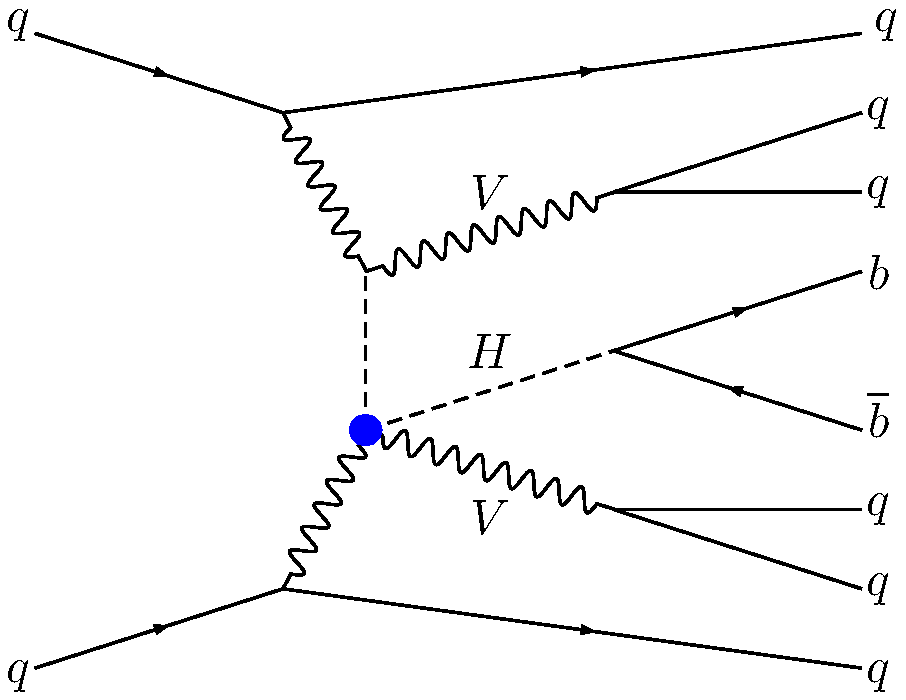
\includegraphics[width=0.45\textwidth]{fig/feynman/vbsvvh/vbsvvh_c2v_allhad.pdf}}
    \quad
    \subfloat{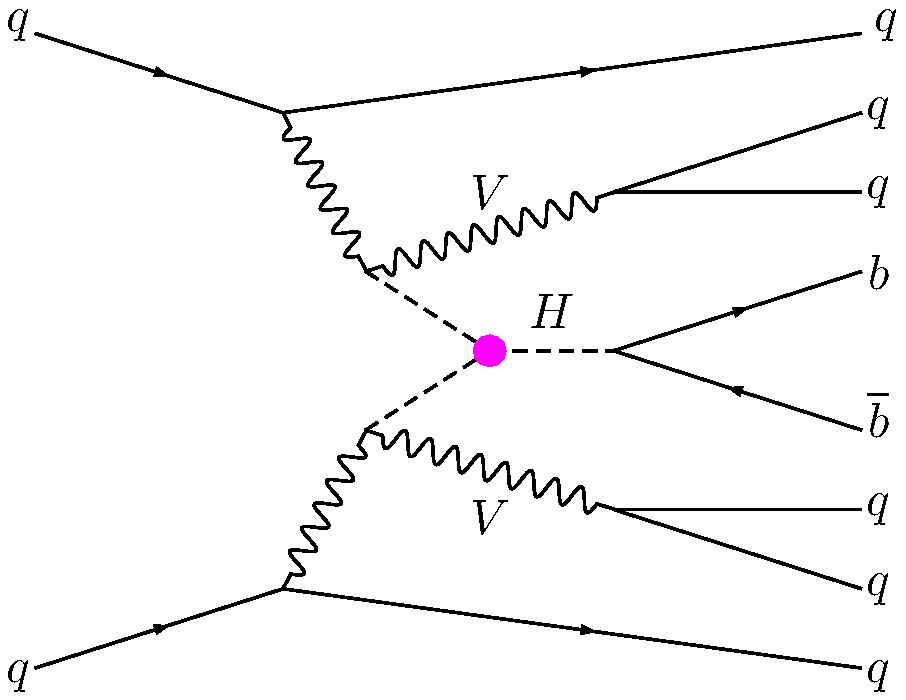
\includegraphics[width=0.45\textwidth]{fig/feynman/vbsvvh/vbsvvh_c3_allhad.pdf}}
    \caption[Leading-order Feynman diagrams for VBS \VVH in the all-hadronic final state]{
        Leading-order Feynman diagrams for VBS production of two vector bosons (V) and one Higgs boson, where the vector bosons decay hadronically and the Higgs boson decays specifically to \PQb quarks. 
        The HHVV coupling \kVV is denoted by a blue circle (\textcolor{blue}{\ding{108}}), and the \HHH coupling \kHHH is denoted by a magenta circle (\textcolor{magenta}{\ding{108}}). 
    }
    \label{fig:vbsvvh_feynman_allhad}
\end{figure}

\subsection{Signal characteristics}
The VBS quarks provide the usual signature: two nearly back-to-back VBS jets have large $|\detajj|$ and \Mjj (Fig.~\ref{fig:vbsvvh_vbs_vars}). 
The boost from BSM values of \kVV is also evident when the \VVH system is reconstructed as three AK8 jets (Fig.~\ref{fig:vbsvvh_fatjet_pts}). 
Moreover, a graph neural network called \ParticleNet can be used to classify each AK8 jet, with negligible misidentification for signal, providing a strong handle for removing the dominant QCD background.
The \ParticleNet regressed mass \MPNet is used to estimate the mass of each AK8 jet, as it has been shown to have better resolution than the other methods, and the clear resonance peaks around the Higgs boson and vector boson masses can be used to separate signal from background, which, in general, does not have such resonances (Fig.~\ref{fig:vbsvvh_fatjet_masses}). 

\begin{figure}[htb]
    \centering
    \subfloat{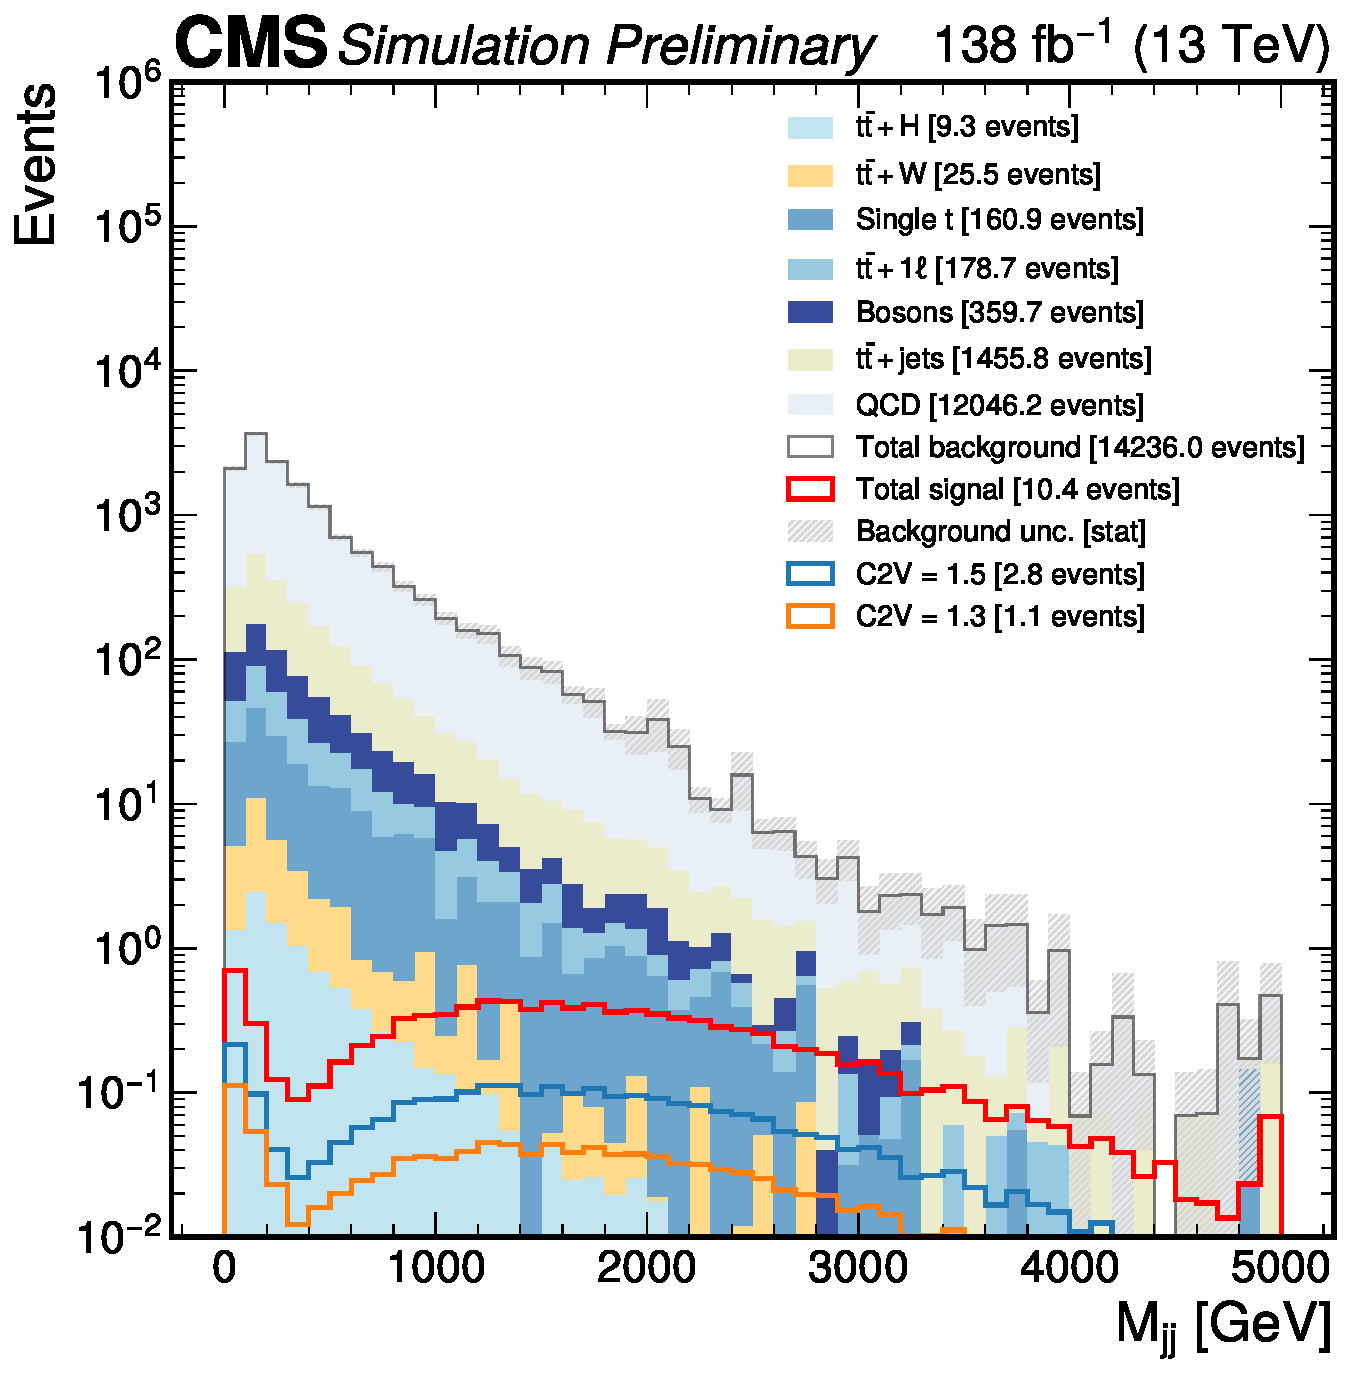
\includegraphics[width=0.45\textwidth]{fig/vbsvvh/M_jj_sig_vs_bkg_stacked_logy.pdf}}
    \qquad
    \subfloat{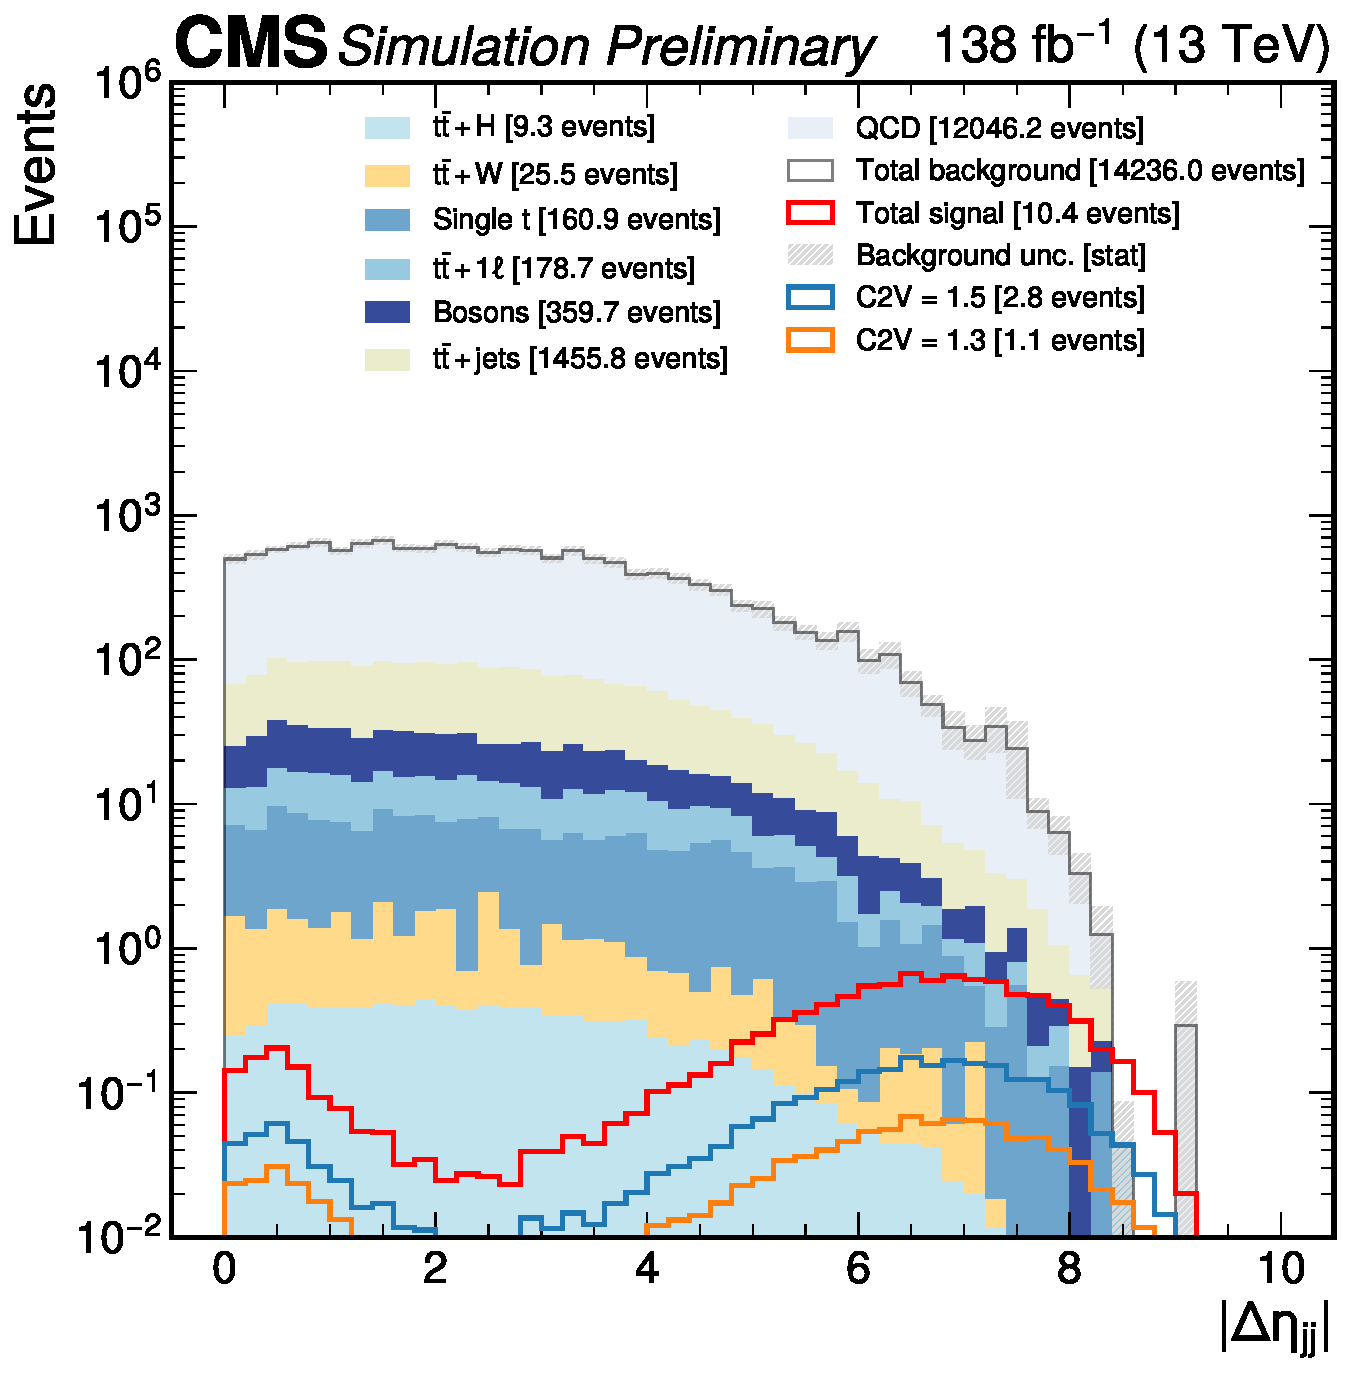
\includegraphics[width=0.45\textwidth]{fig/vbsvvh/abs_deta_jj_sig_vs_bkg_stacked_logy.pdf}}
    \caption[The \Mjj and \detajj distribution for the VBS jets]{
        The invariant mass \Mjj (left) and pseudorapidity separation \detajj (right) of the VBS jets plotted after the Preselection is applied. 
        The main signal MC ($\kVV = 2$) is plotted in red alongside $\kVV = 1.5$ and $\kVV = 1.3$ for comparison. 
    }
    \label{fig:vbsvvh_vbs_vars}
\end{figure}

\begin{figure}[htb]
    \centering
    \subfloat{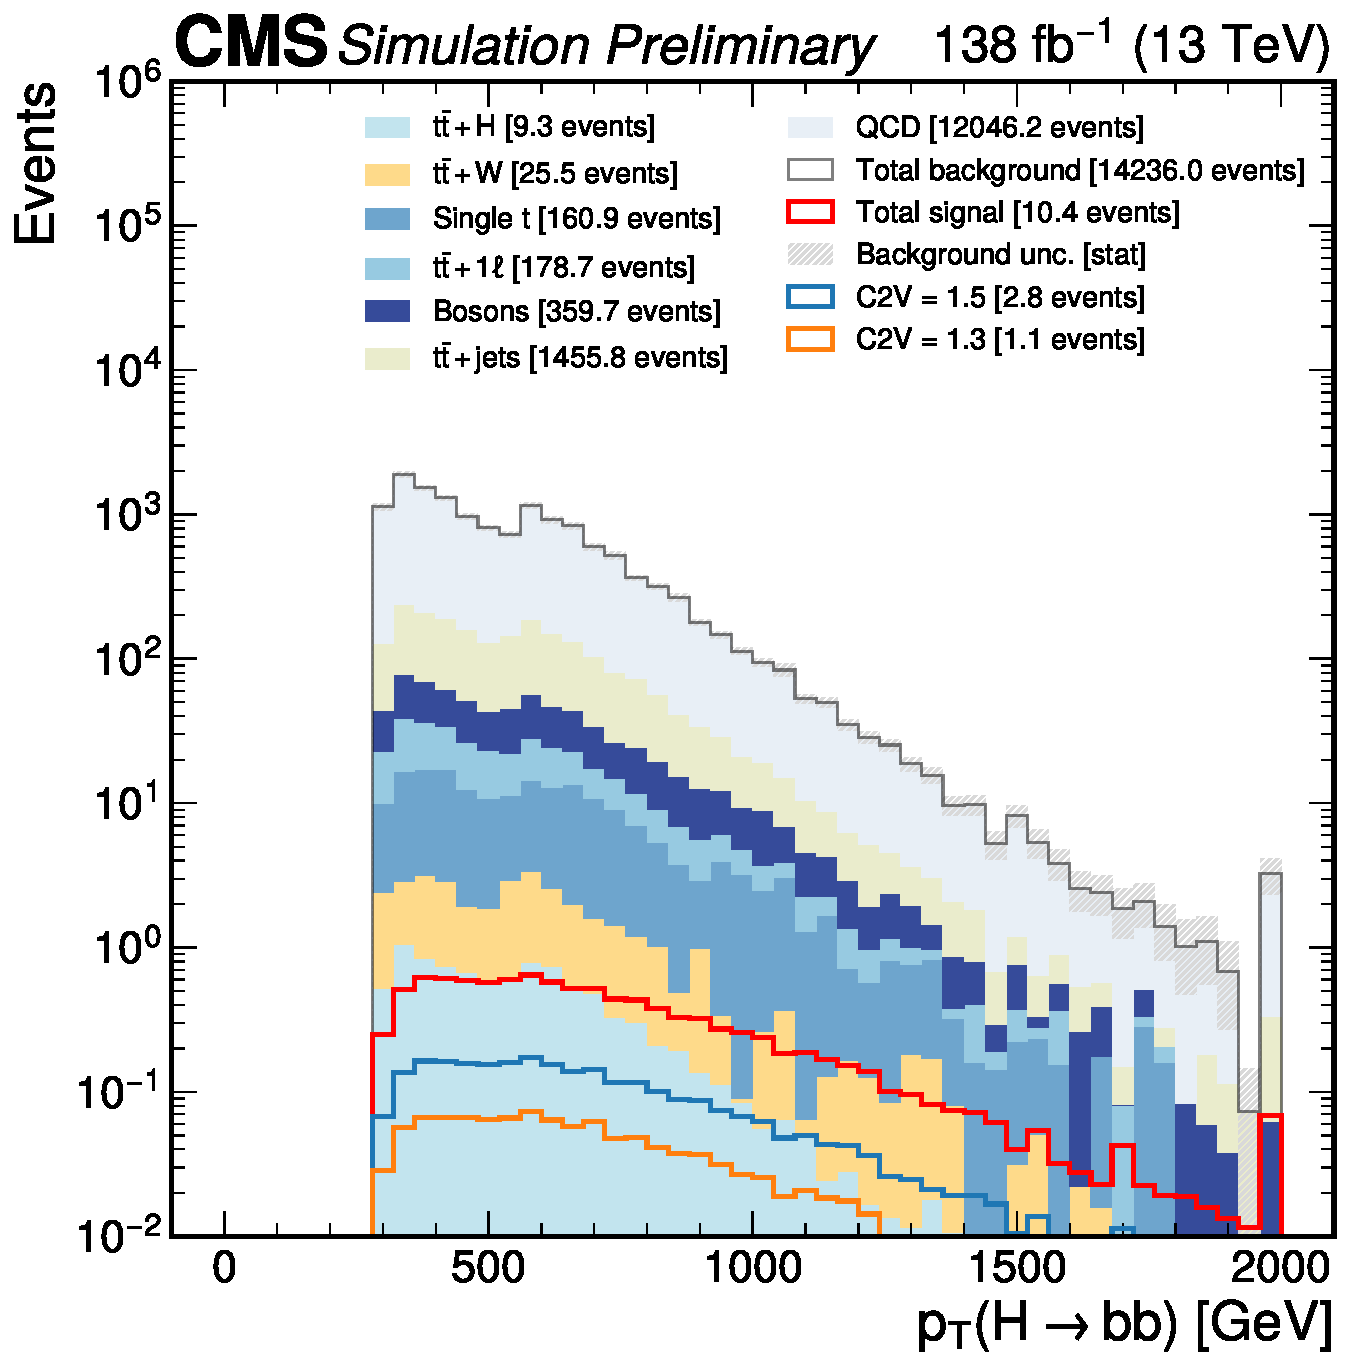
\includegraphics[width=0.32\textwidth]{fig/vbsvvh/hbbfatjet_pt_sig_vs_bkg_stacked_logy.pdf}}
    \subfloat{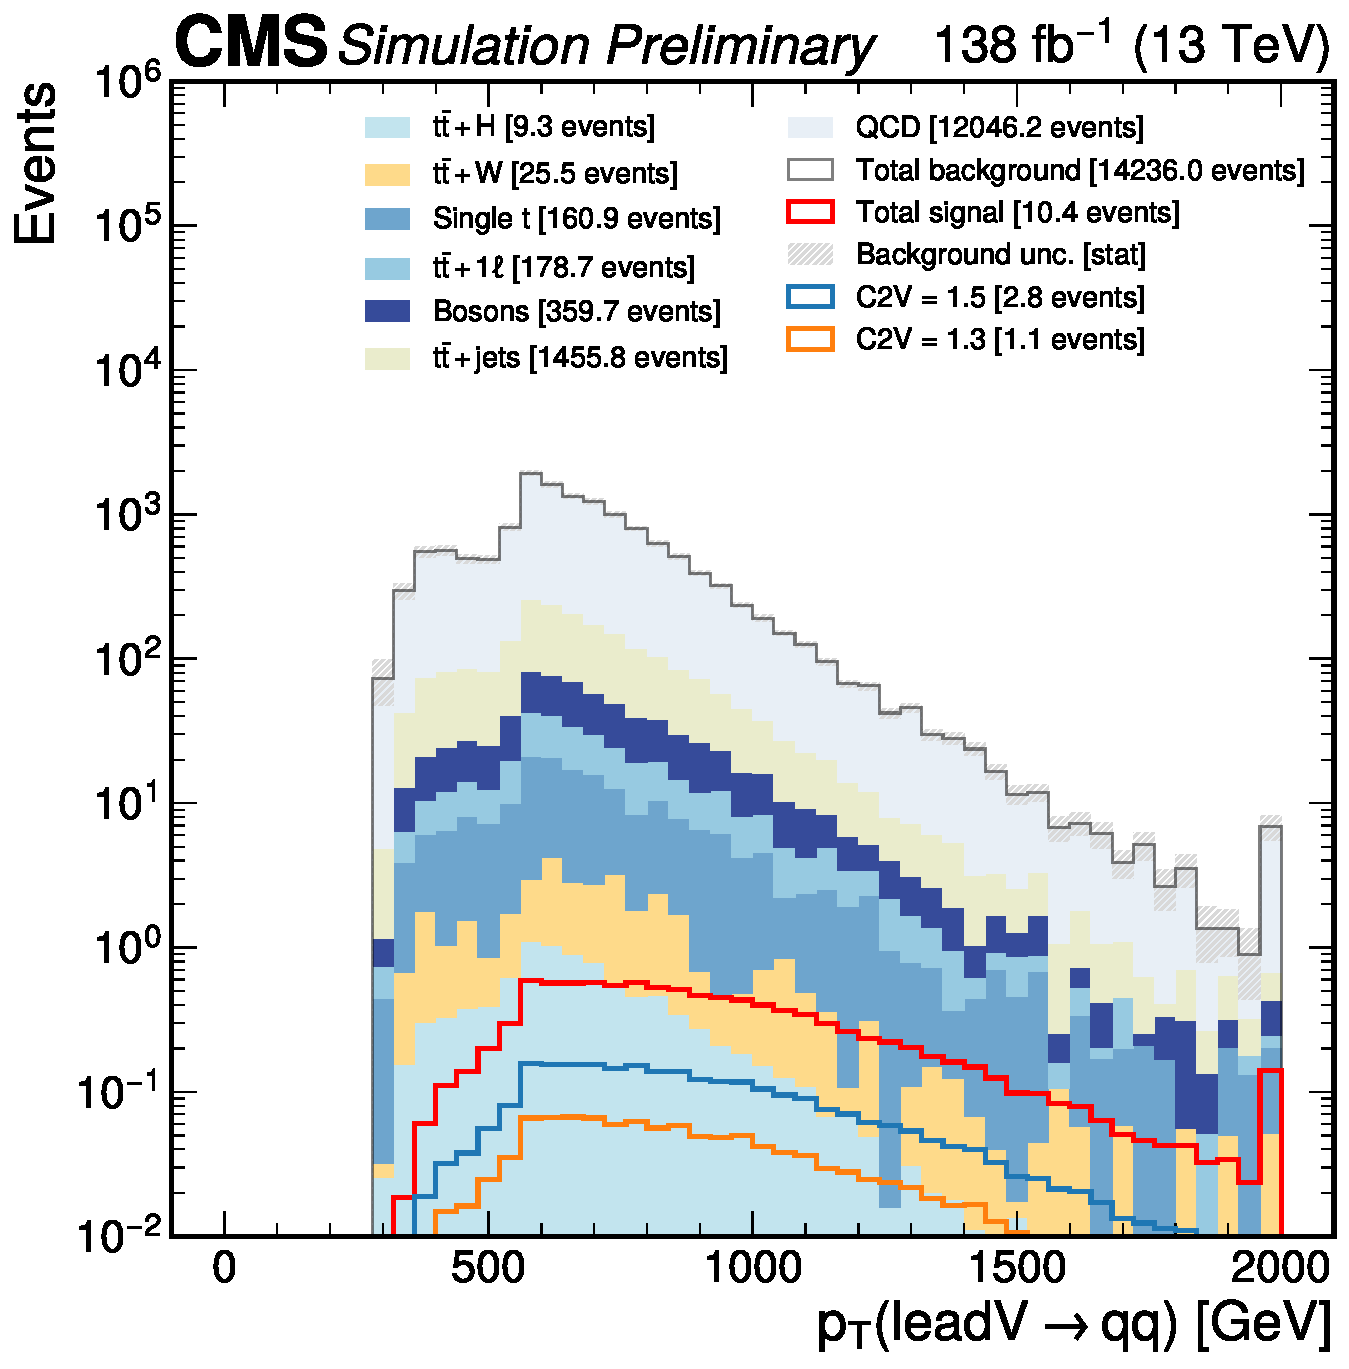
\includegraphics[width=0.32\textwidth]{fig/vbsvvh/ld_vqqfatjet_pt_sig_vs_bkg_stacked_logy.pdf}}
    \subfloat{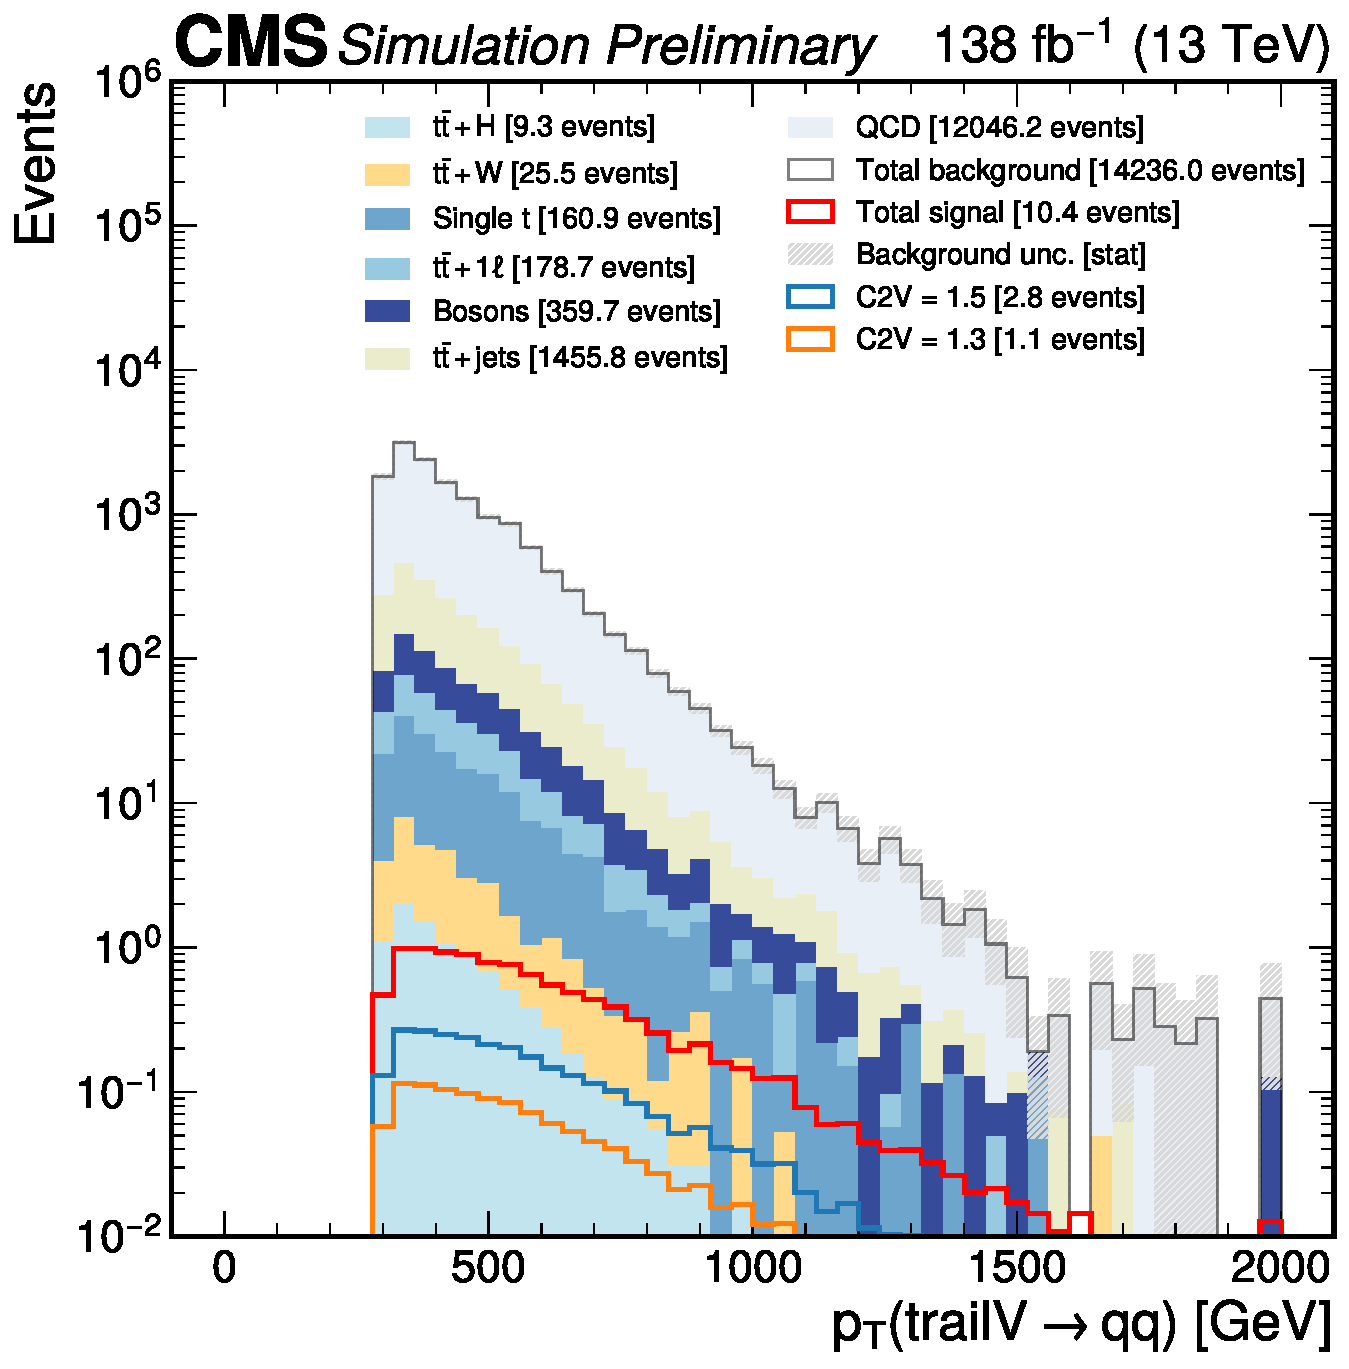
\includegraphics[width=0.32\textwidth]{fig/vbsvvh/tr_vqqfatjet_pt_sig_vs_bkg_stacked_logy.pdf}}
    \caption[The \pt distribution for each of the three VBS \VVH AK8 jets]{
        The \pt of the \Htobb (left), leading \Vtoqq (center), and trailing \Vtoqq (right) AK8 jets plotted after the Preselection is applied. 
        The main signal MC ($\kVV = 2$) is plotted in red alongside $\kVV = 1.5$ and $\kVV = 1.3$ for comparison. 
    }
    \label{fig:vbsvvh_fatjet_pts}
\end{figure}

\begin{figure}[htb]
    \centering
    \subfloat{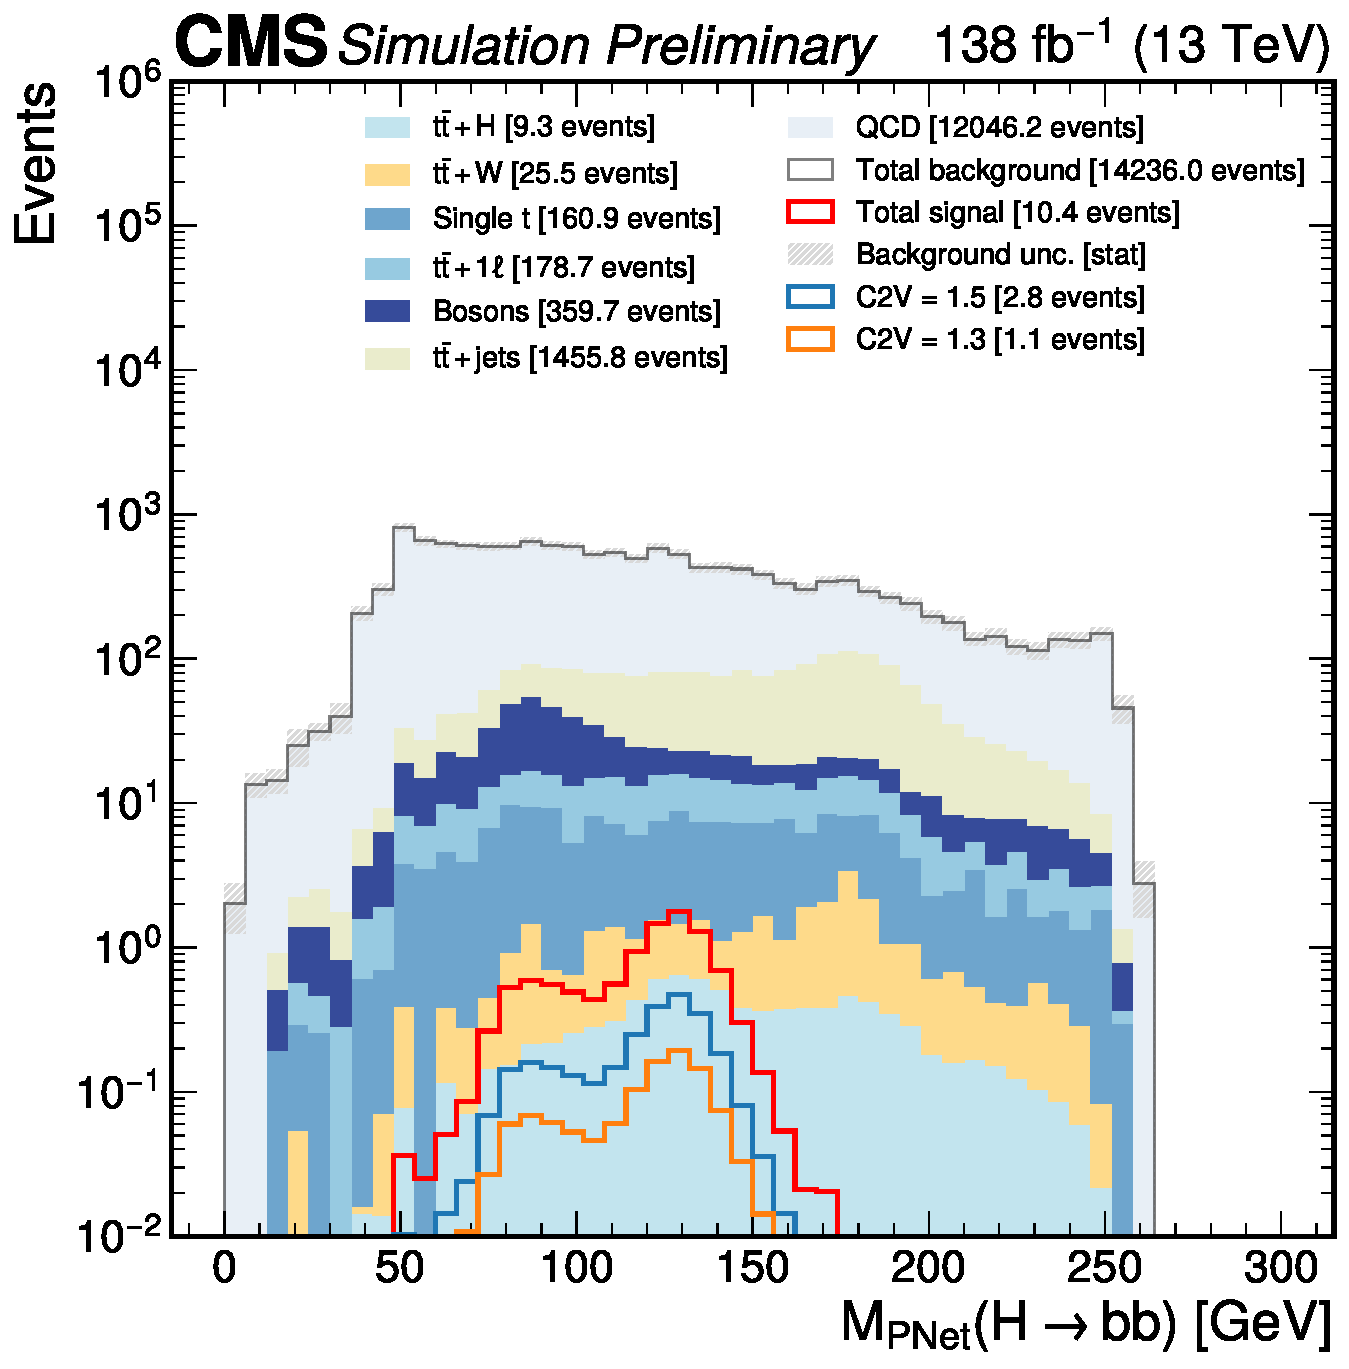
\includegraphics[width=0.32\textwidth]{fig/vbsvvh/hbbfatjet_mass_sig_vs_bkg_stacked_logy.pdf}}
    \subfloat{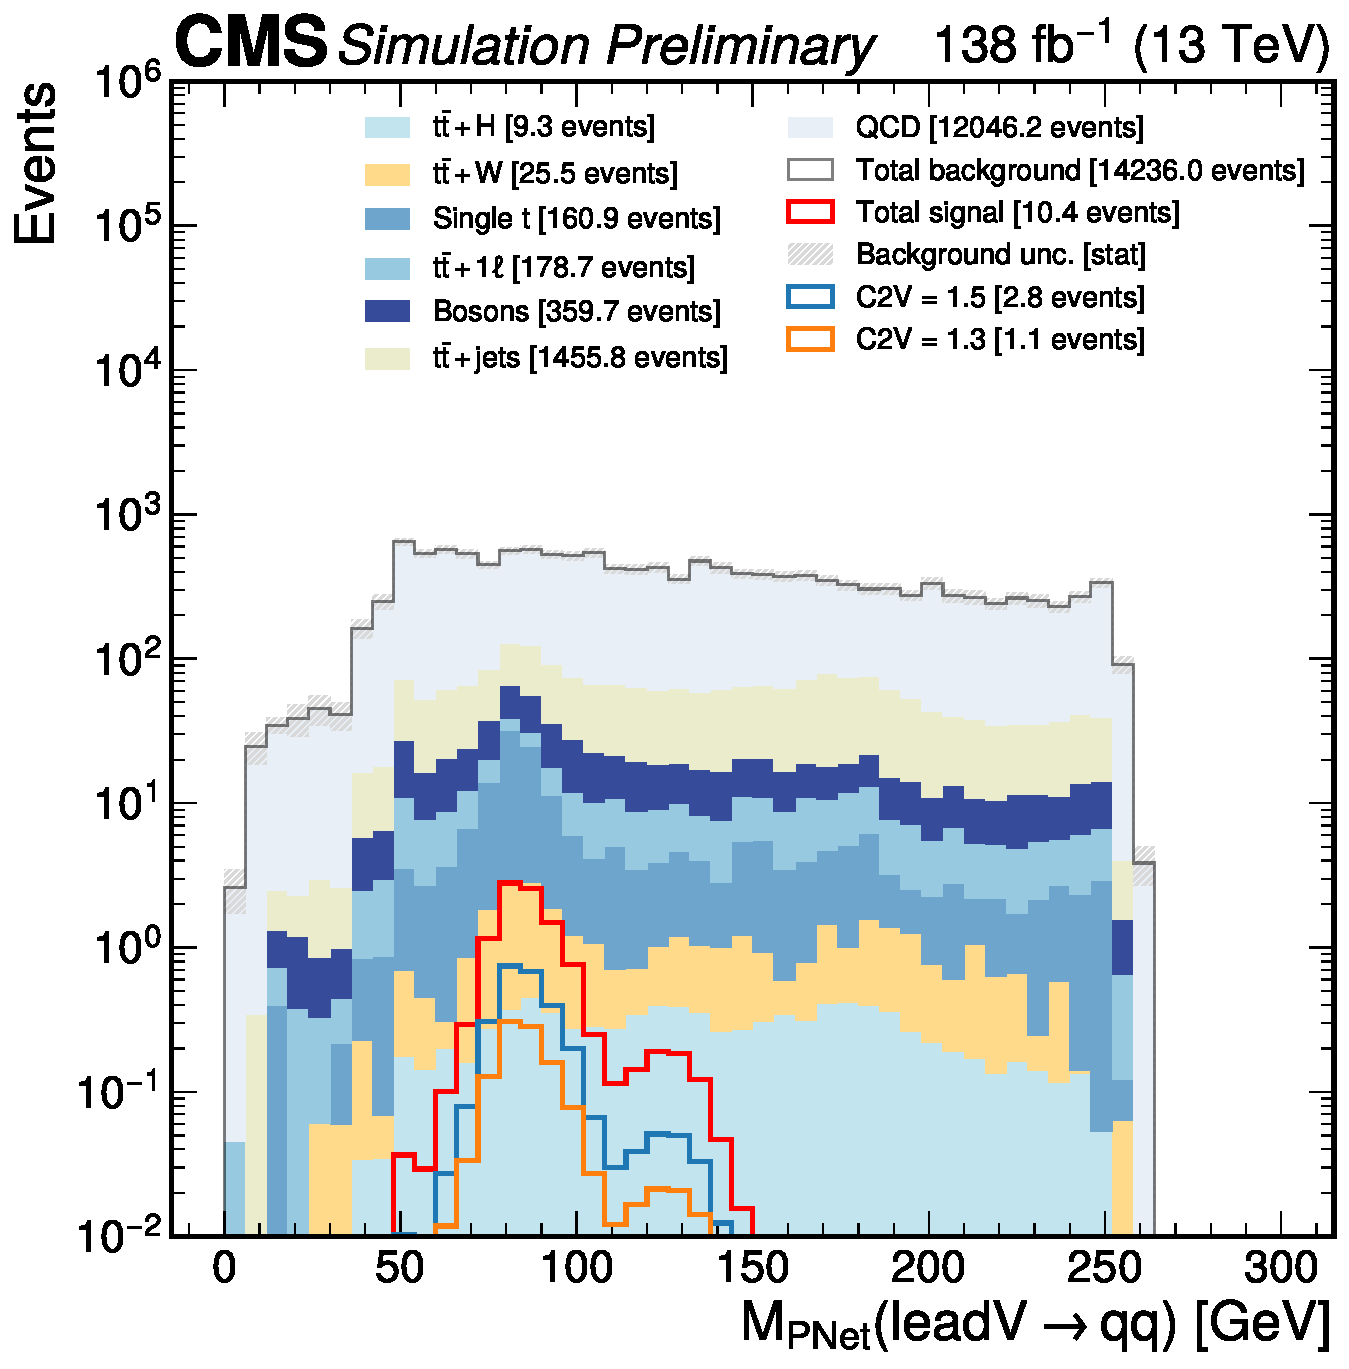
\includegraphics[width=0.32\textwidth]{fig/vbsvvh/ld_vqqfatjet_mass_sig_vs_bkg_stacked_logy.pdf}}
    \subfloat{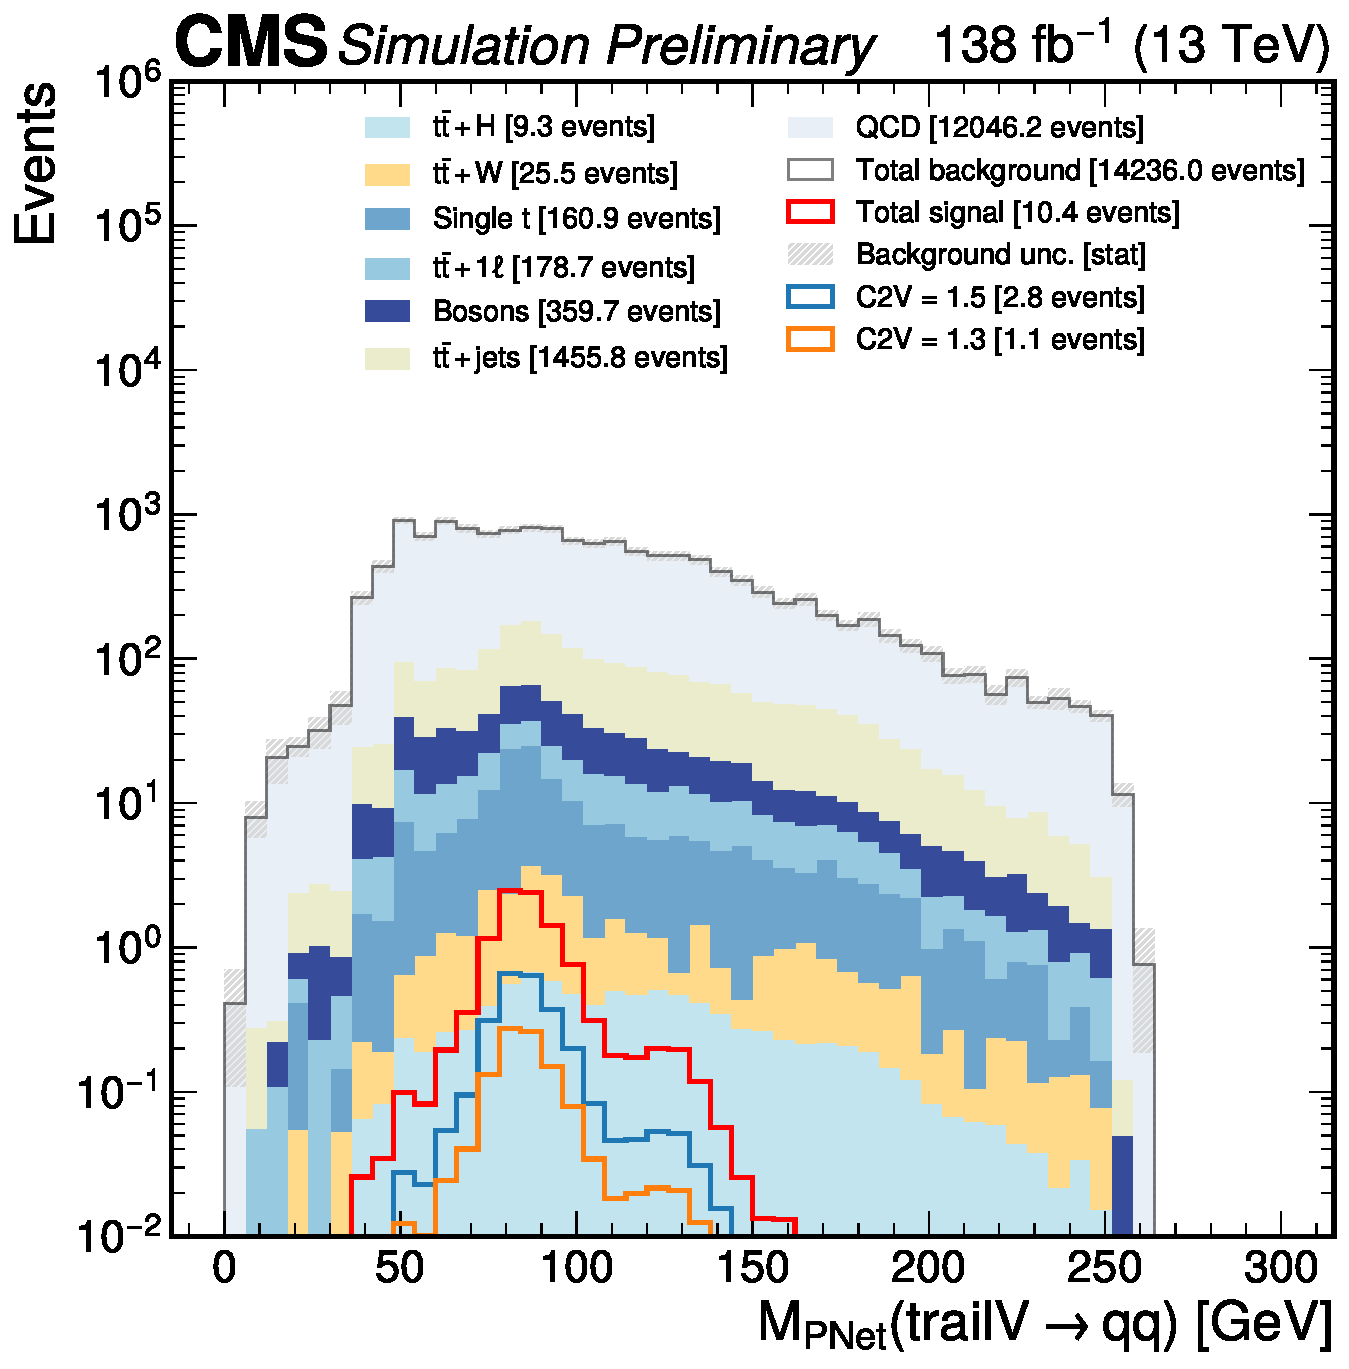
\includegraphics[width=0.32\textwidth]{fig/vbsvvh/tr_vqqfatjet_mass_sig_vs_bkg_stacked_logy.pdf}}
    \caption[The \ParticleNet regressed mass distribution for each of the three VBS \VVH AK8 jets]{
        The \ParticleNet regressed masses \MPNet of the \Htobb (left), leading \Vtoqq (center), and trailing \Vtoqq (right) AK8 jets plotted after the Preselection is applied. 
        The main signal MC ($\kVV = 2$) is plotted in red alongside $\kVV = 1.5$ and $\kVV = 1.3$ for comparison. 
    }
    \label{fig:vbsvvh_fatjet_masses}
\end{figure}

\section{The backgrounds}
The main background in this analysis comes from QCD multijet production (Fig.~\ref{fig:qcd_multijet}), wherein the quarks and gluons in the colliding protons interact and produce more quarks and gluons. 
This is the most common process at the LHC, and it dominates the background for many analyses that target an all-hadronic final state. 
The largest sub-leading backgrounds are \ttbar production (Fig.~\ref{fig:ttbar_allhad}) and multi-boson production in all-hadronic final states. 
All of these backgrounds simply produce many jets that can, by random chance, pass our \Htobb selections, or have genuine vector bosons that decay hadronically. 

\begin{figure}[htb]
    \centering
    \subfloat[QCD multijet]{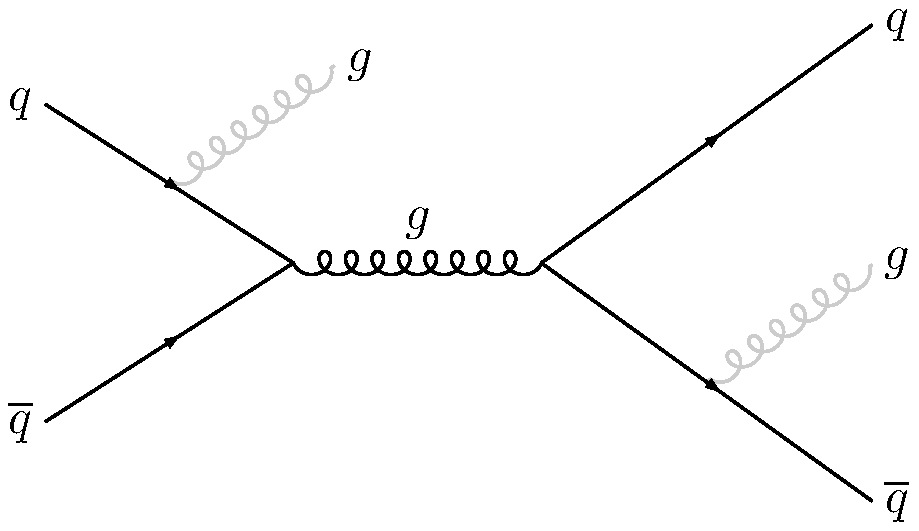
\includegraphics[width=0.4\textwidth]{fig/feynman/other/qcd_multijet.pdf}\label{fig:qcd_multijet}}
    \quad
    \subfloat[\ttbar in the all-hadronic final state]{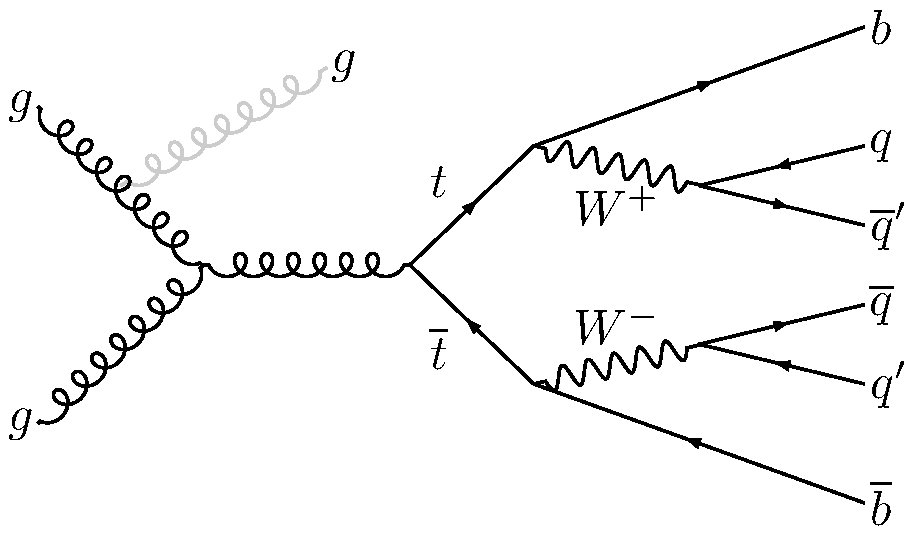
\includegraphics[width=0.4\textwidth]{fig/feynman/ttbar/ttbar_allhad_extraJet_ggF.pdf}\label{fig:ttbar_allhad}}
    \caption[Feynman diagrams for QCD multijet and \ttbar production]{
        Feynman diagram for QCD multijet production (left) and \ttbar production in the all-hadronic final state (right), the leading and subleading backgrounds, respectively, for the VBS \VVH all-hadronic analysis. 
    }
    \label{fig:vbsvvh_bkgs} % sub-leading background (W+jets and single top)
\end{figure}

\subsection{QCD \ParticleNet resampling}
From Fig.~\ref{fig:vbsvvh_dataMC_fatjet_scores_noCorr}, it is clear that the data and MC distributions for the \ParticleNet scores used in this analysis do not fully agree. 
This is not an issue for the final result, as the background estimation is fully data-driven. 
However, for training any classifier for this analysis, such as a boosted decision tree (BDT) or deep neural network (DNN), better modeling would result in more events passing the Preselection, and therefore being available for training.

\begin{figure}[htb]
    \centering
    \subfloat{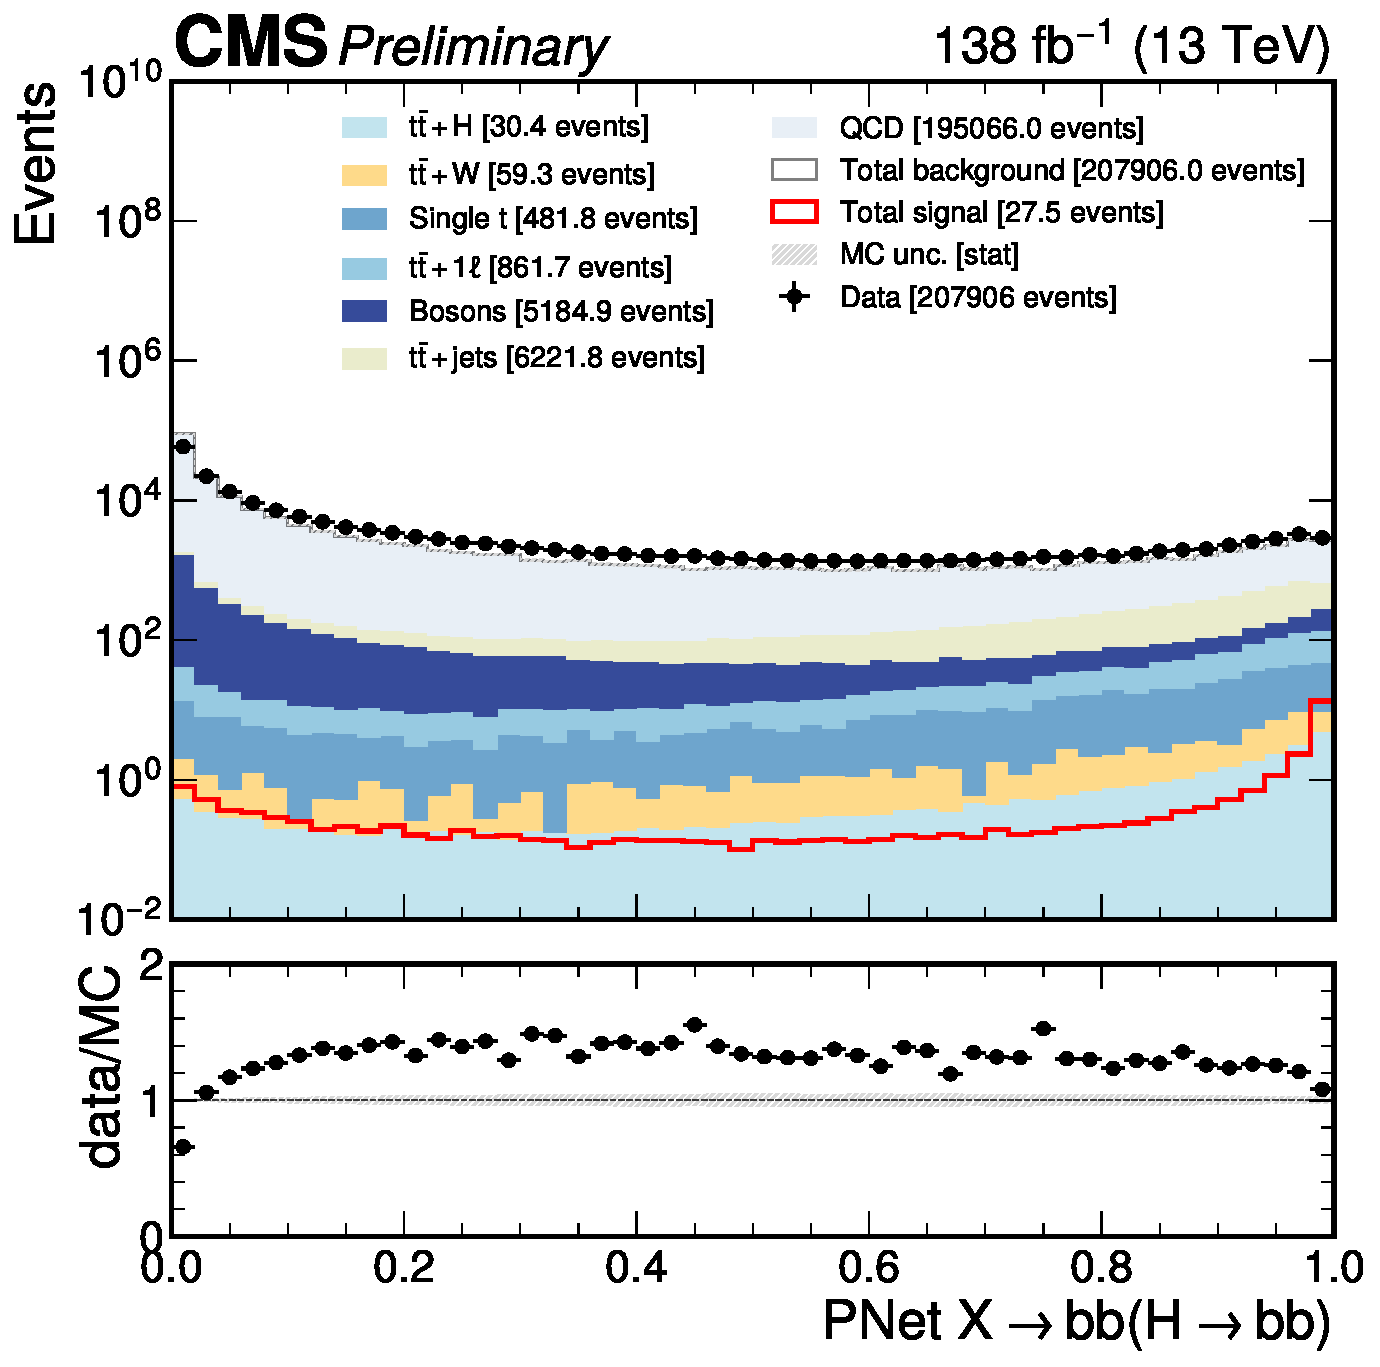
\includegraphics[width=0.32\textwidth]{fig/vbsvvh/noqcdfix_hbbfatjet_xbb_data_vs_mc_log_objsel.pdf}}
    \subfloat{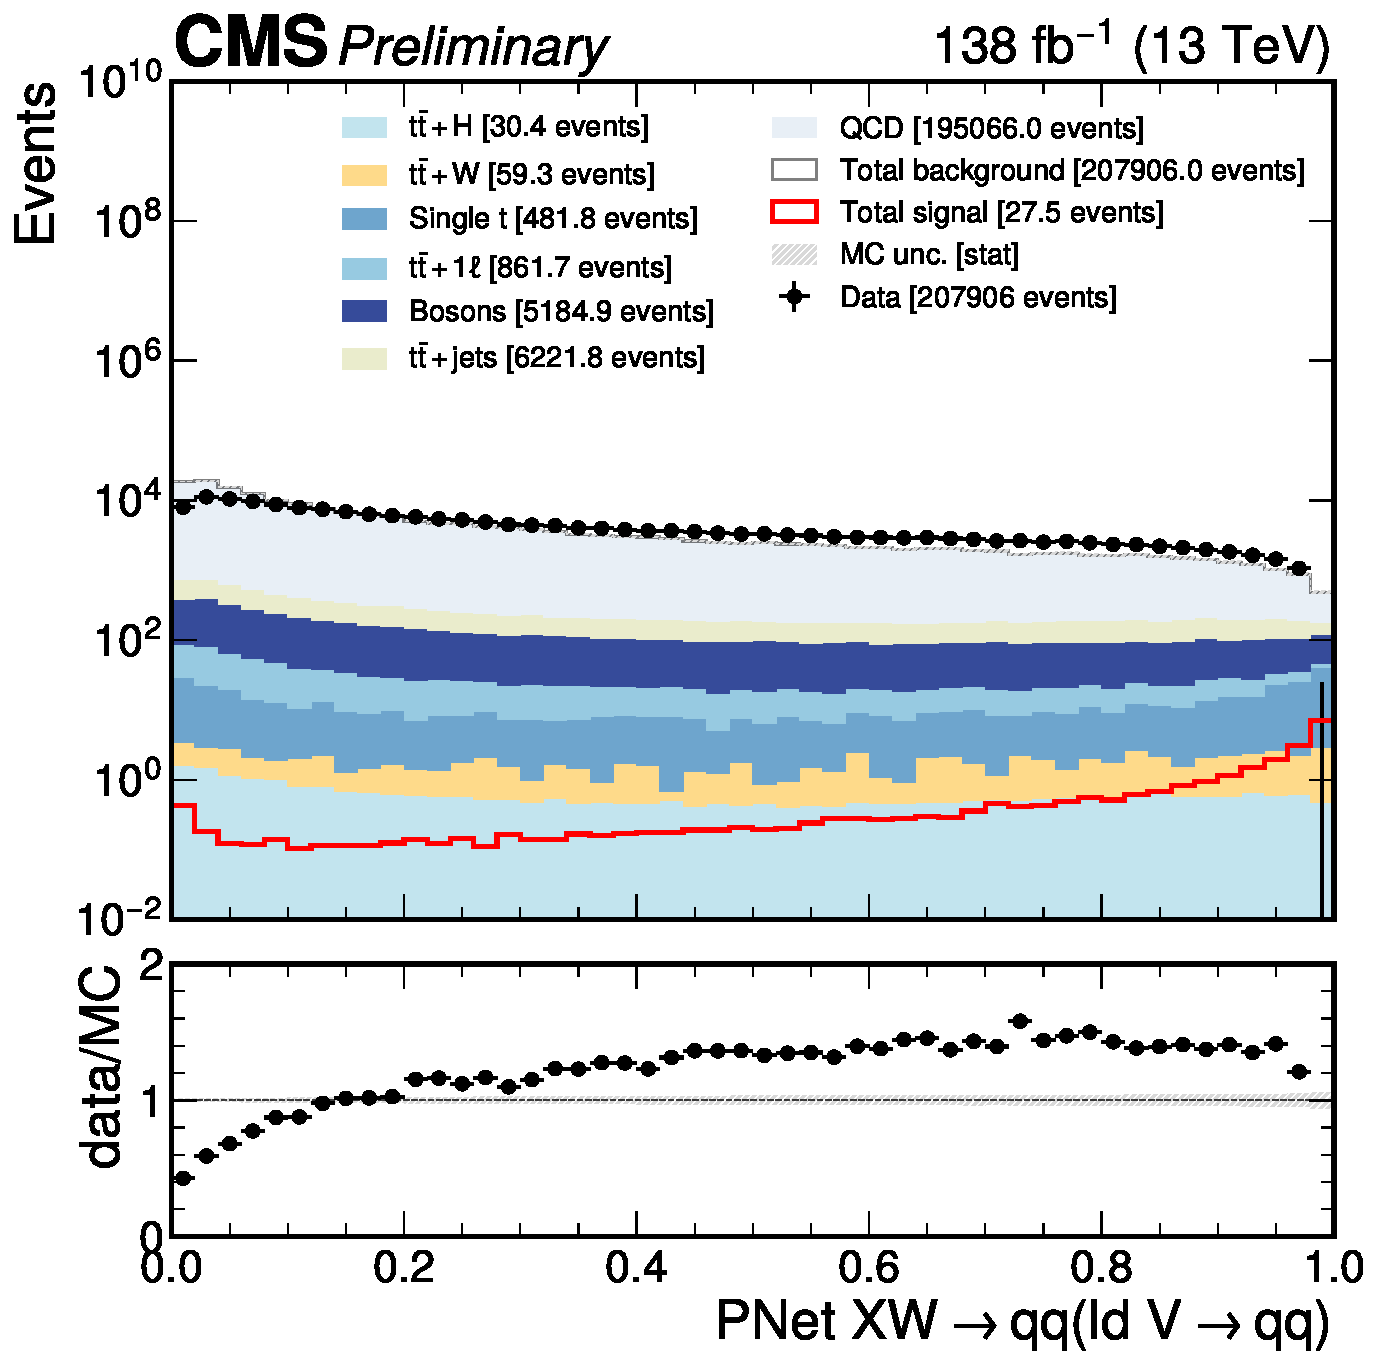
\includegraphics[width=0.32\textwidth]{fig/vbsvvh/noqcdfix_ld_vqqfatjet_xwqq_data_vs_mc_log_objsel.pdf}}
    \subfloat{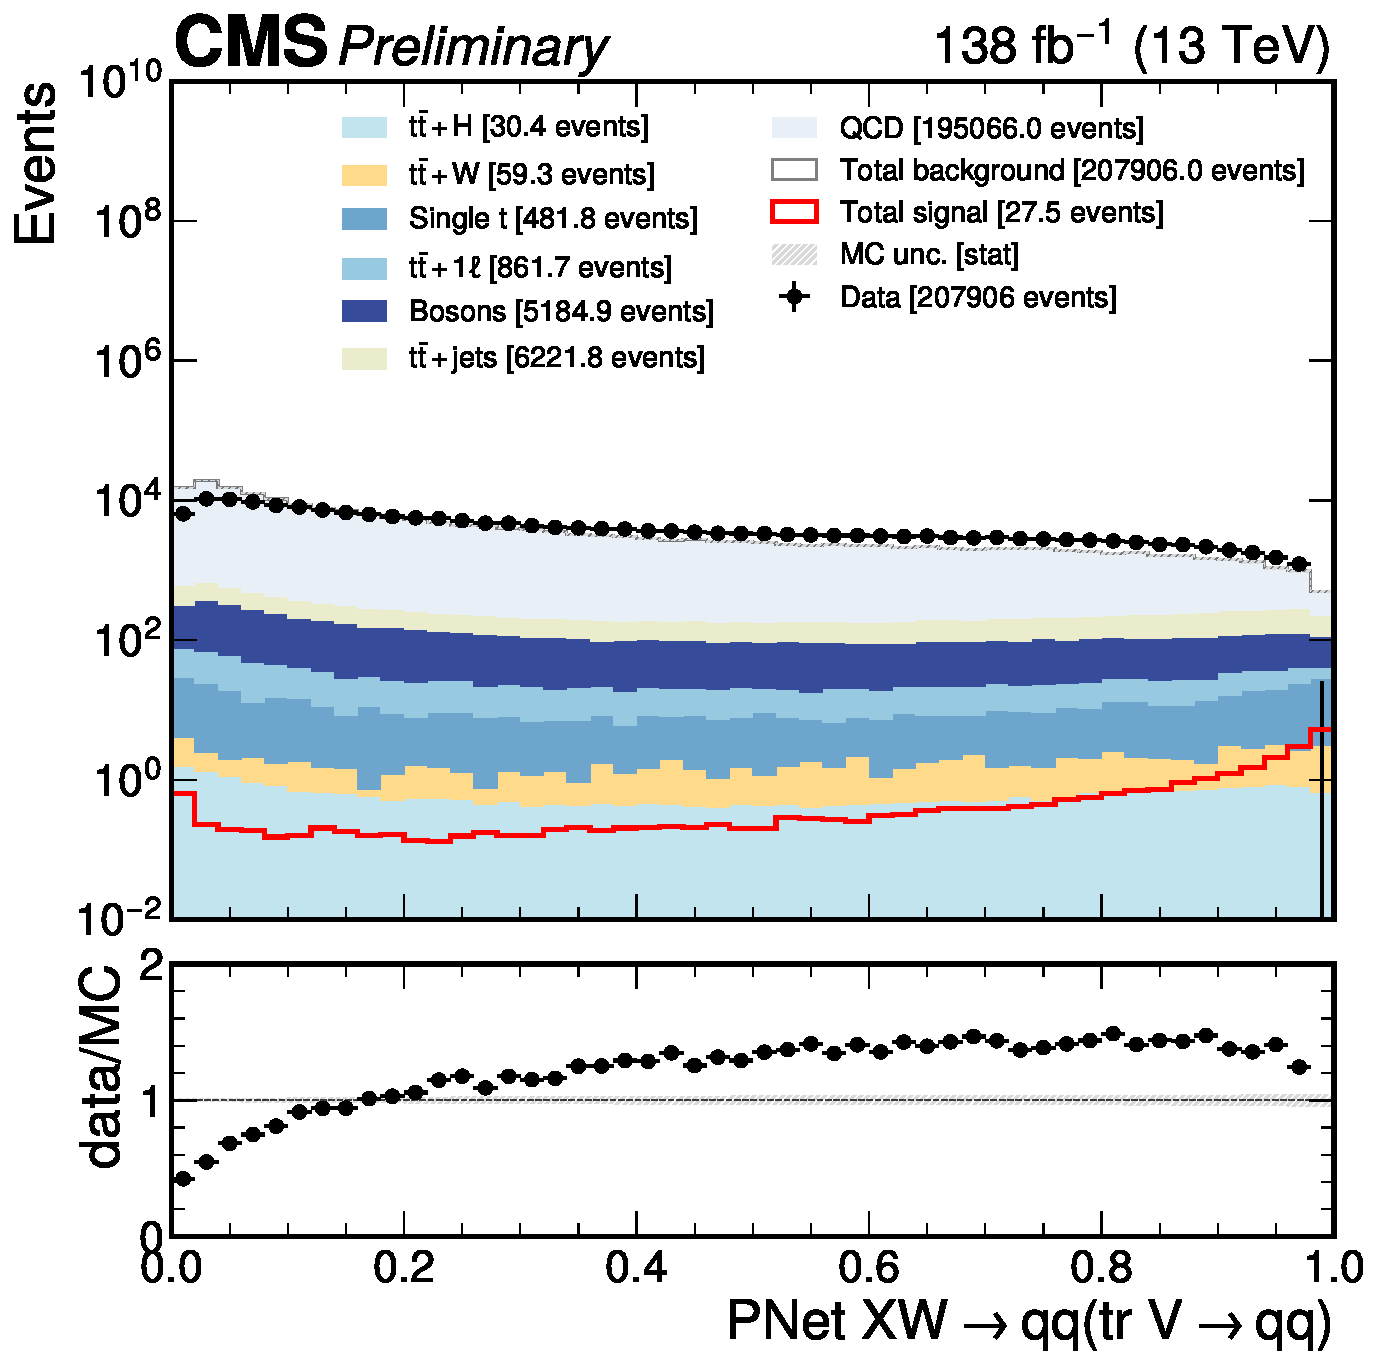
\includegraphics[width=0.32\textwidth]{fig/vbsvvh/noqcdfix_tr_vqqfatjet_xwqq_data_vs_mc_log_objsel.pdf}}
    \caption[The \ParticleNet score distribution for each of the three VBS \VVH AK8 jets plotted in data and MC before QCD resampling]{
        The \ParticleNet scores for the \Htobb (left), leading \Vtoqq (center), and trailing \Vtoqq (right) AK8 jets plotted after the analysis objects are selected. 
        The main signal MC ($\kVV = 2$) is plotted in red alongside $\kVV = 1.5$ and $\kVV = 1.3$ for comparison. 
    }
    \label{fig:vbsvvh_dataMC_fatjet_scores_noCorr}
\end{figure}

To address this, the following resampling procedure is used to correct the \ParticleNet score shape for QCD MC. 
Only the scores for the QCD jets undergo this procedure, and the rest of the minor backgrounds are subtracted from the data distributions used for the resampling.
First, the following assumptions are made:
\begin{enumerate}
    \item A mass-decorrelated \ParticleNet score for a given AK8 jet should be fundamentally described by a probability density function $\mathcal{P}$, namely $\mathcal{P}_{\Xtobb}$ and $\mathcal{P}_{\XWtoqq}$ for the \ParticleNet \Xtobb and \XWtoqq scores, respectively.
    \item $\mathcal{P}$ should be the same regardless of how many AK8 jets are in the event.
    \item The \ParticleNet score is not correlated to the jet kinematic properties used later in the analysis. 
\end{enumerate}
Assumption 1 is the common statistical interpretation of a histogram; that is, $\mathcal{P}$ can be approximated by histogramming the \ParticleNet score for every AK8 jet in an event and normalizing it to unity. 
Assumption 2 is less trivial. 
In our case, we need to verify that events with 3 AK8 jets to contain the same kinds of AK8 jets as an event with 2 AK8 jets. 
This is not guaranteed, as events with different AK8 jet multiplicity may involve different physics. 
For QCD events in this analysis, however, it can be seen in Fig.~\ref{fig:vbsvvh_pnetpdf} that Assumption 2 holds, as the \textit{PDFs} in 3 AK8 jet events approximately match the 2 AK8 jet events in data (with non-QCD events taken from MC subtracted out).
Therefore, the properly binned $\mathcal{P}$ derived in data for 2-AK8-jet events can be sampled to replace the \ParticleNet scores in 3-AK8-jet events. 
In order to account for the correlation in this resampling, we bin the \ParticleNet \Xtobb score in \pt. 

The \ParticleNet \XWtoqq score, on the other hand, must be binned in the \Xtobb score and \pt, since the \Xtobb score is included indirectly in the calculation of the \XWtoqq score. 
The leading \Xtobb score is also picked first, thus potentially further biasing the correlation among the scores.
The replacement is performed for each AK8 jet via the following prescription:
\begin{enumerate}
    \item Get AK8 jet \pt
    \item Sample $\mathcal{P}_{\Xtobb}$ for the appropriate \pt bin
    \item Replace AK8 jet \Xtobb score with one randomly sampled from $\mathcal{P}_{\Xtobb}$
    \item Get $\mathcal{P}_{\XWtoqq}$ for the appropriate \pt, \Xtobb score bin
    \item Replace AK8 jet \XWtoqq score with one randomly sampled from $\mathcal{P}_{\XWtoqq}$
\end{enumerate}
After replacing the AK8 jet scores in events with 3 AK8 jets, the \ParticleNet score distribution agreement between data and MC improves significantly (Fig.~\ref{fig:vbsvvh_dataMC_fatjet_scores}), doubling the number of raw QCD MC events that pass the Preselection.

\begin{figure}[htb]
    \centering
    \subfloat{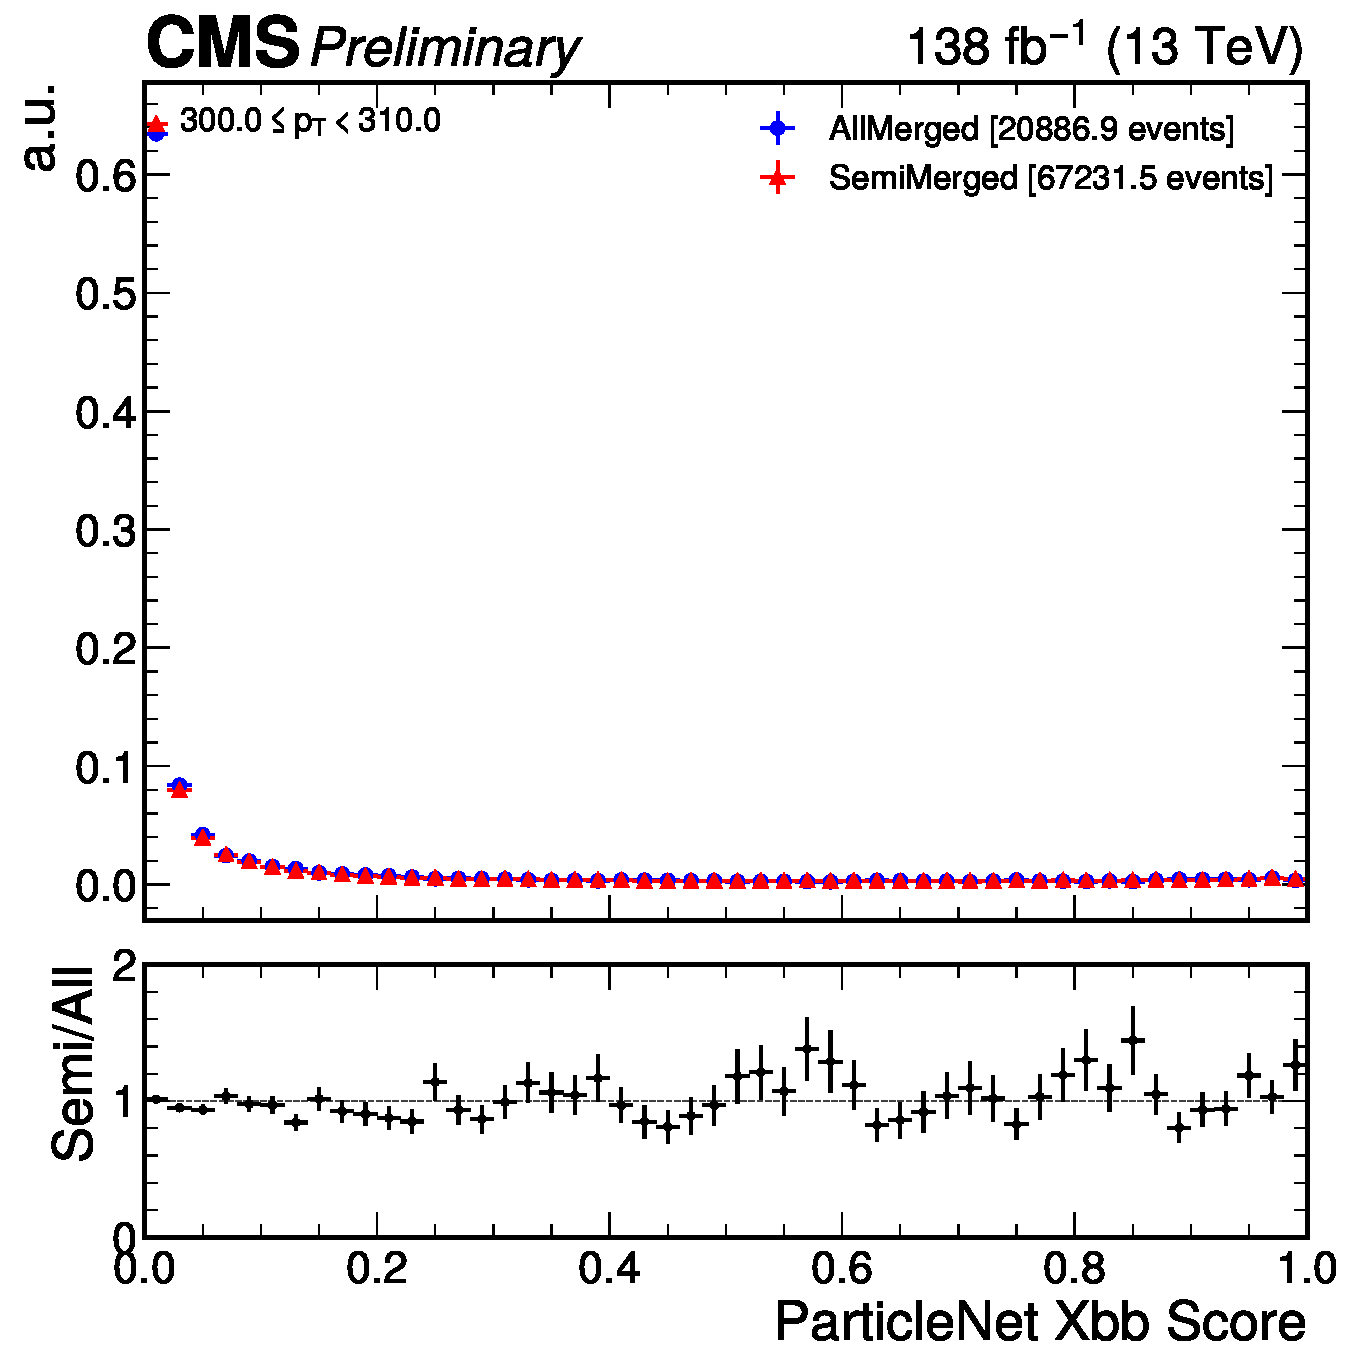
\includegraphics[width=0.45\textwidth]{fig/vbsvvh/qcdfix/data_minus_nonqcd_xbb_1D_pdf_xbin0.pdf}}
    \qquad
    \subfloat{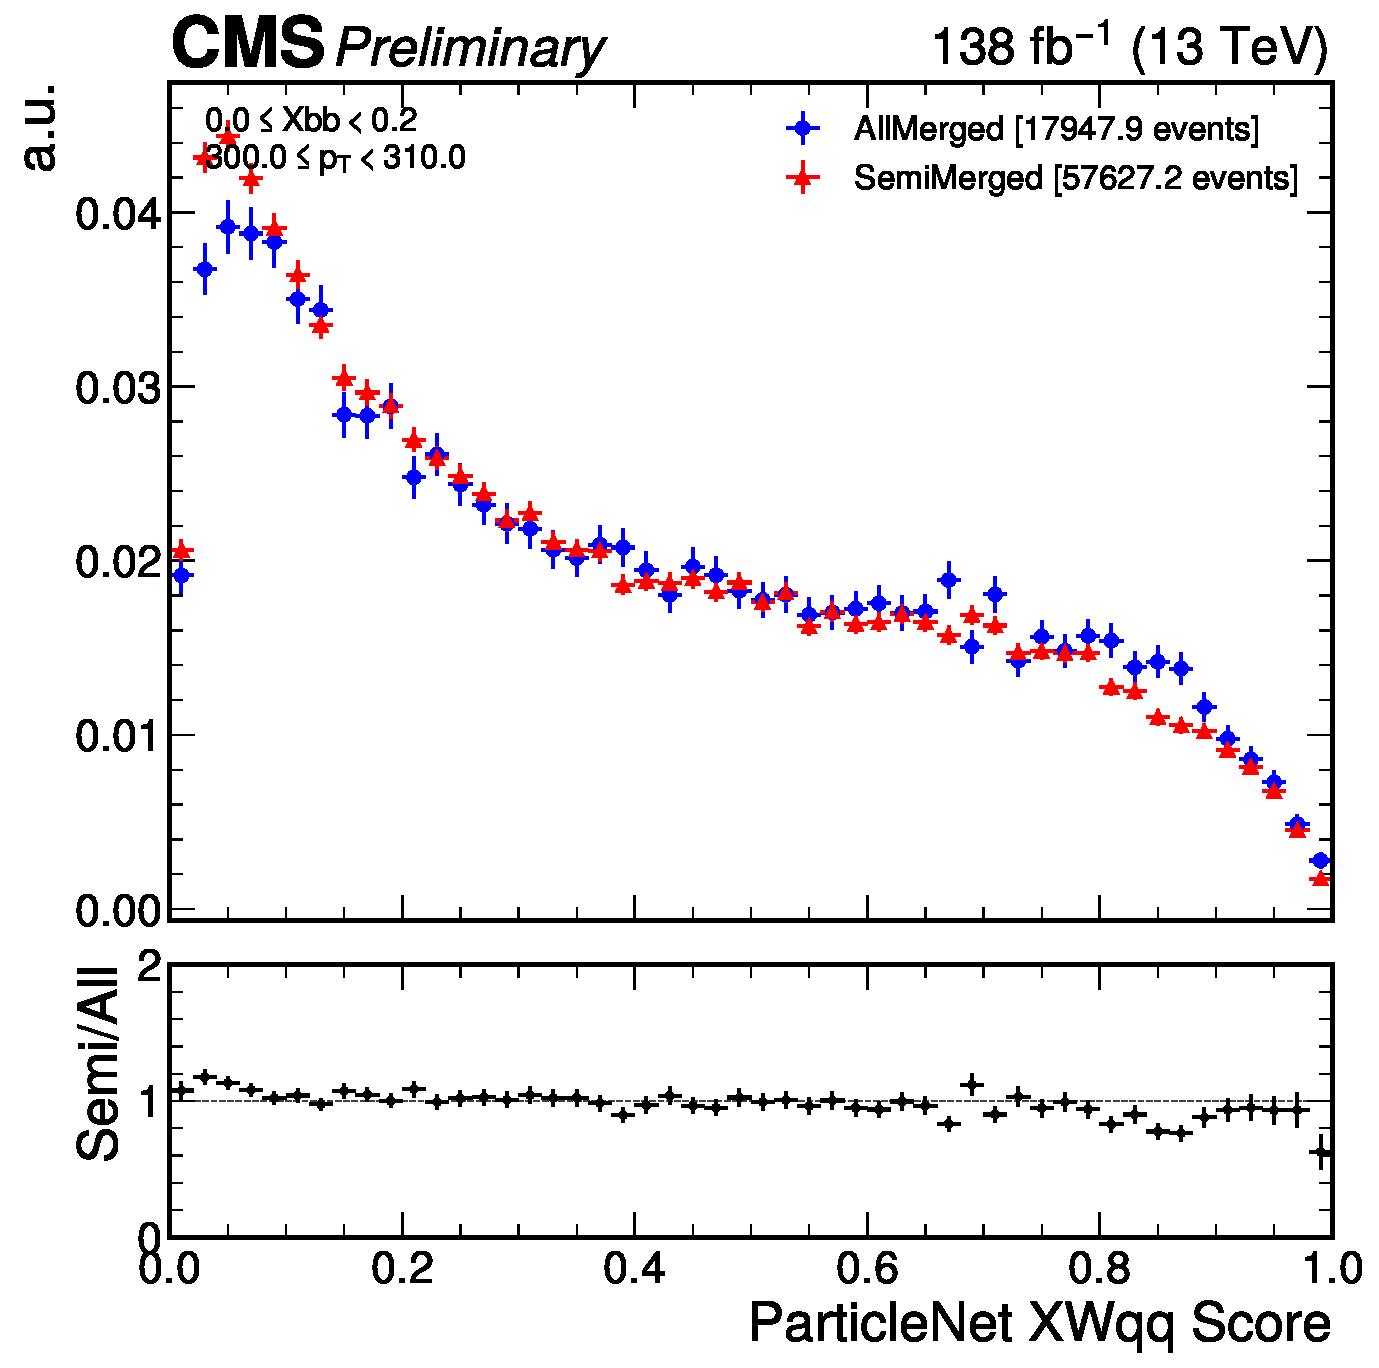
\includegraphics[width=0.45\textwidth]{fig/vbsvvh/qcdfix/data_minus_nonqcd_xwqq_2D_pdf_xbin0_ybin0.pdf}}
    \caption[The approximation of the \ParticleNet probability density functions]{
        The approximation of the \ParticleNet probability density functions plotted for the \Xtobb score in one bin of \pt (left) and the \XWtoqq score in one bin of \pt and \Xtobb (right). 
    }
    \label{fig:vbsvvh_pnetpdf}
\end{figure}

\begin{figure}[htb]
    \centering
    \subfloat{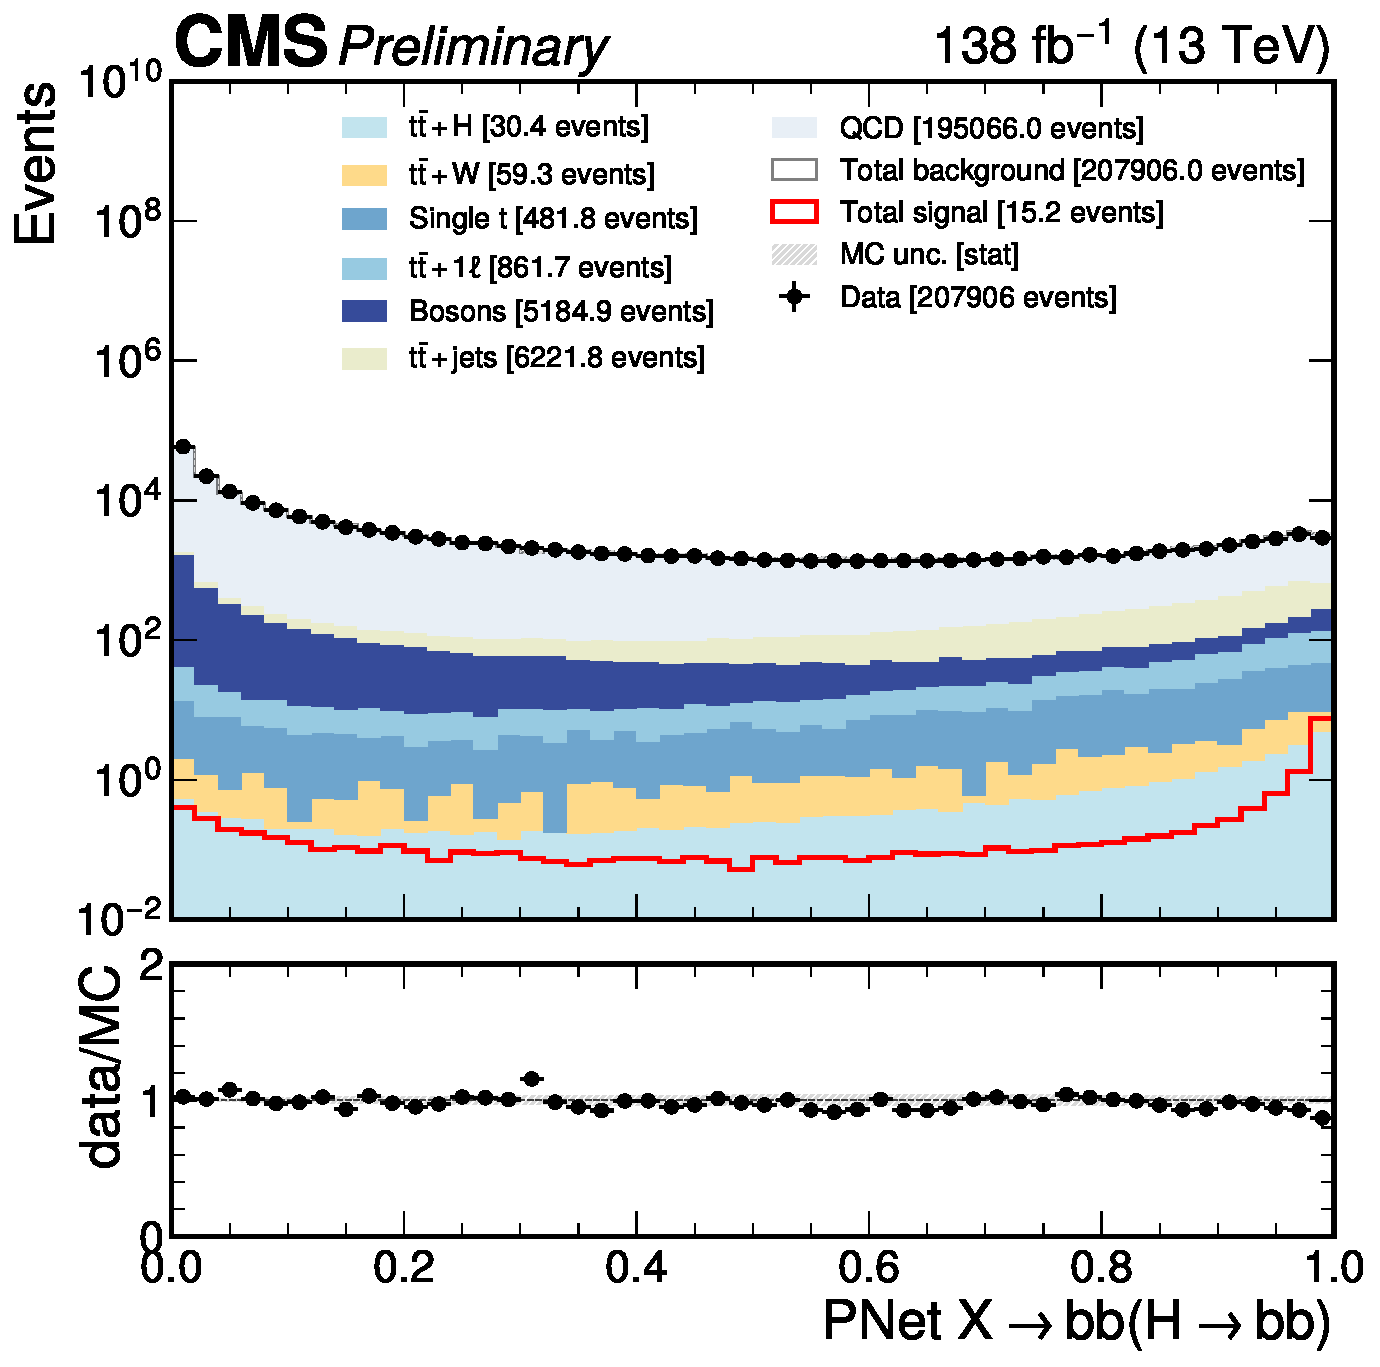
\includegraphics[width=0.32\textwidth]{fig/vbsvvh/hbbfatjet_xbb_data_vs_mc_log_objsel.pdf}}
    \subfloat{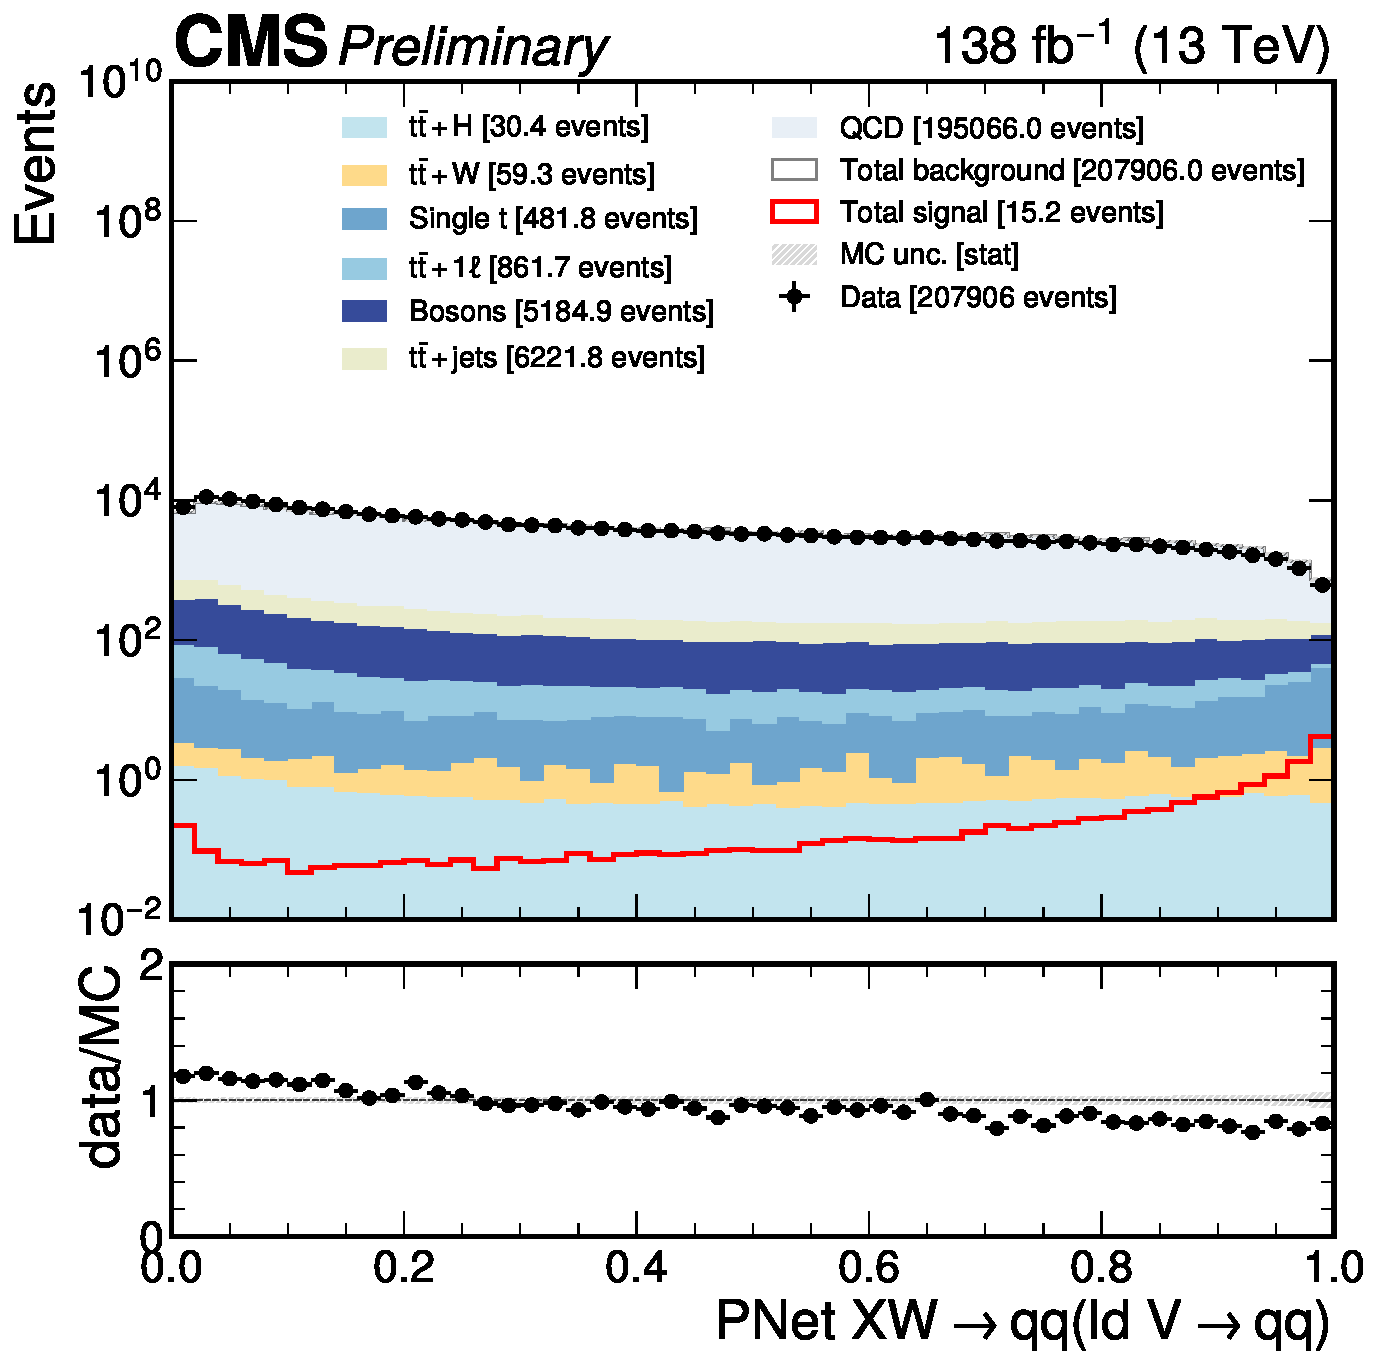
\includegraphics[width=0.32\textwidth]{fig/vbsvvh/ld_vqqfatjet_xwqq_data_vs_mc_log_objsel.pdf}}
    \subfloat{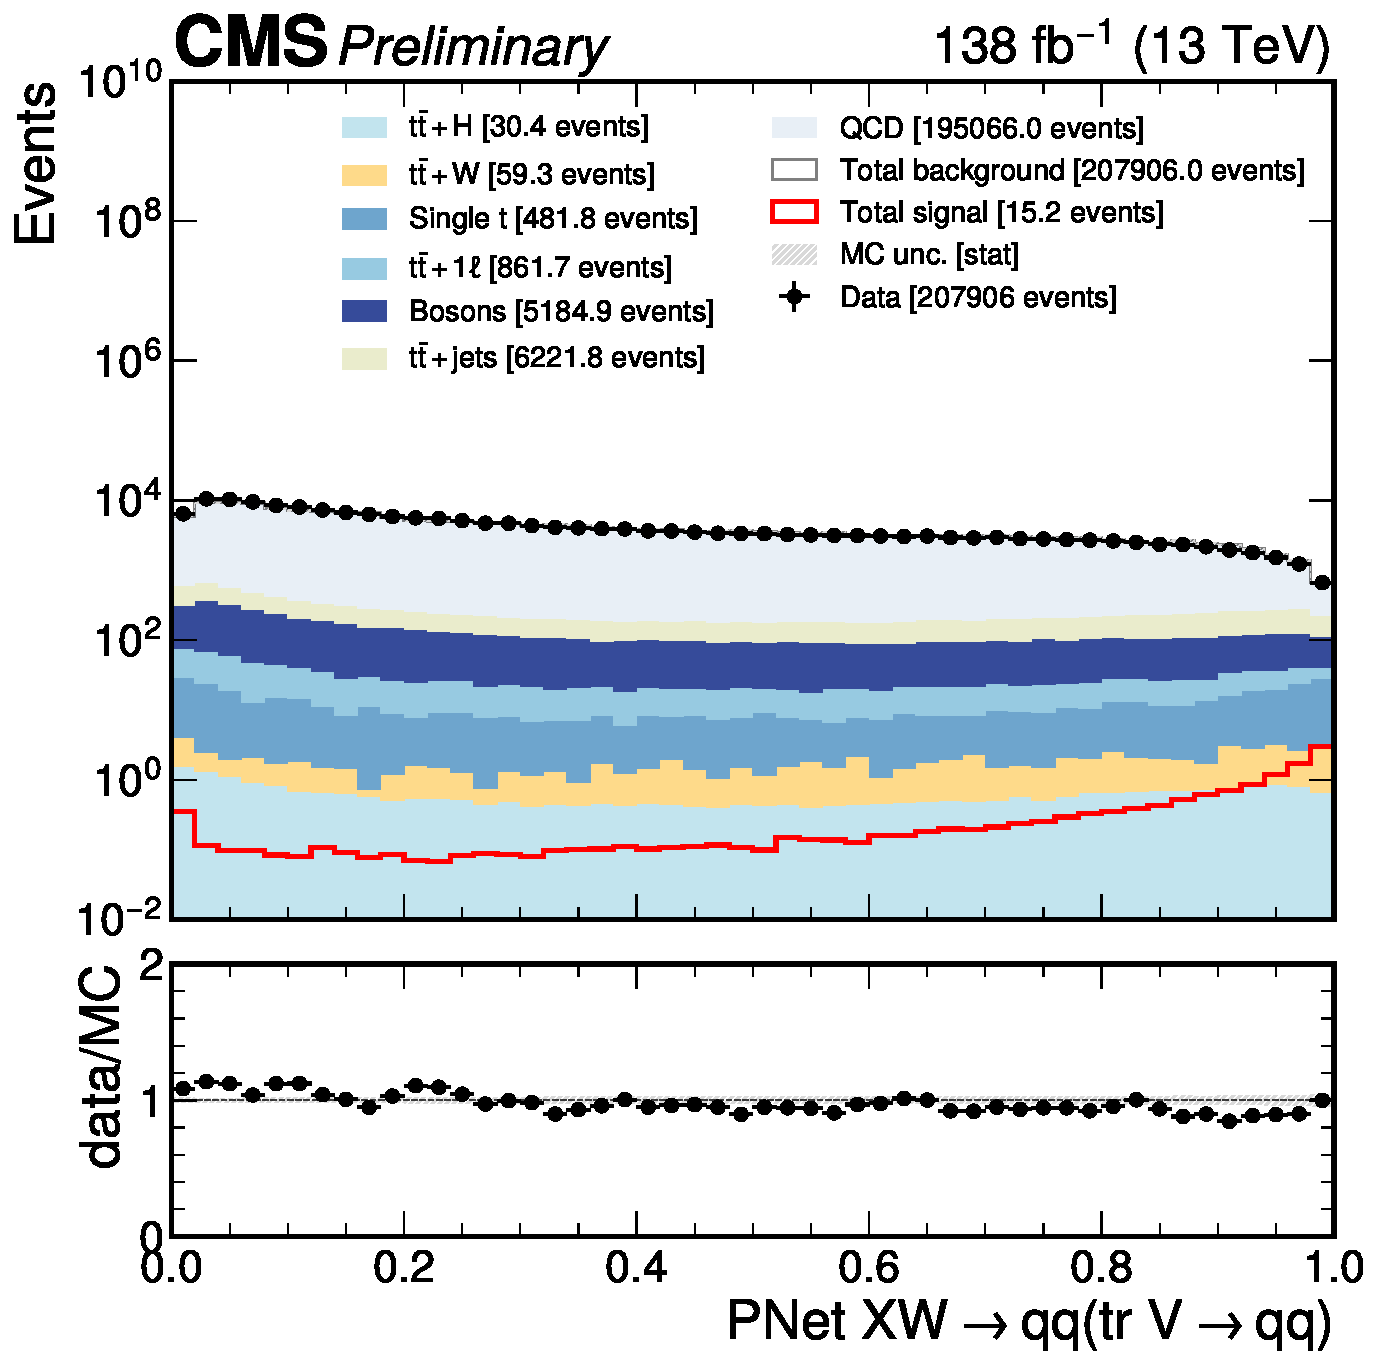
\includegraphics[width=0.32\textwidth]{fig/vbsvvh/tr_vqqfatjet_xwqq_data_vs_mc_log_objsel.pdf}}
    \caption[The \ParticleNet score distribution for each of the three VBS \VVH AK8 jets plotted in data and MC after QCD resampling]{
        The \ParticleNet scores for the \Htobb (left), leading \Vtoqq (center), and trailing \Vtoqq (right) AK8 jets plotted after the analysis objects are selected and the QCD resampling is applied. 
        The main signal MC ($\kVV = 2$) is plotted in red alongside $\kVV = 1.5$ and $\kVV = 1.3$ for comparison. 
    }
    \label{fig:vbsvvh_dataMC_fatjet_scores}
\end{figure}

\section{Event selection}

\subsection{Triggers and preselection}
Because the entire final state is composed of jets, the jet \HT triggers are applied, where \HT is ``hadronic transverse energy,'' or the sum of the \pt of every jet in the event. 
Moreover, since the jets considered in this analysis are expected to be highly boosted, these triggers are 100\% efficient for signal events. 
The same event-level filters used to remove detector noise and unphysical events in the analysis described in the previous chapter are applied also in this analysis. 

Also like the previous analysis, a loose selection referred to as the ``Preselection'' is applied to select the final state of interest. 
First, events are required to have zero leptons passing the veto lepton ID. 
This orthogonalizes the all-hadronic channel from the other channels that are analyzed separately. 
The event must have at least three AK8 jets, where the leading AK8 jet is required to have $\pt > 500\GeV$ (while for all of them the \pt threshold is 250\GeV) such that the analysis is on the \HT-binned trigger threshold. 
Finally, the event is also required to have two AK4 jets, following the VBS jet selection scheme detailed in Section~\ref{sec:vbsjets}.
Then, the AK8 jet with the highest \ParticleNet Xbb score is selected as the \Htobb candidate. 
The next two AK8 jets are selected as the \Vtoqq candidates, sorted (leading vs. trailing) by \pt.
With the AK8 jets thus tagged, a very loose selection is applied to the \ParticleNet scores: the \Htobb candidate is required to have a \ParticleNet \Xtobb score greater than 0.5, while the \Vtoqq candidates are each required to have a \ParticleNet \XWtoqq score greater than 0.3.

\subsection{\ABCDNet}
The signal region would preferably be accompanied by a valid data-driven background estimation method while also being optimized for maximal significance, since the dominant background is multijet QCD.
Because this is a common analysis scenario, a machine learning (ML) method has been proposed to satisfy both requirements at once~\cite{AutoABCD}. 
This method has been used already in some published work, e.g. Ref.~\cite{CMS:2022cpe}. 
In particular, a DNN is trained to serve as one of the ``arms'' of a traditional ABCD background estimation. 
Critically, a \dCorrSq term is added to the loss function ($\mathcal{L}$) that trains the DNN to be decorrelated with the other arm:
\begin{equation}
    \mathcal{L}[f(\vec{x})] = \mathcal{L}_\mathrm{BCE}[f(\vec{x}, y)] + \lambda\dCorrSq_{y=0}[f(\vec{x}), X_0]
\end{equation}
where $\vec{x}$ is the input vector, $y$ is the truth label (1 for signal, 0 for background), $\lambda$ is a tunable parameter for controlling the size of the decorrelation term, and $X_0$ is the decorrelation target, which the analyzer is free to choose.
Binary Cross Entropy ($\mathcal{L}_\mathrm{BCE}$) is used in our analysis, however any loss function $\mathcal{L}$ could in principle be used in its place.
The \dCorrSq term is the ``distance correlation,'' a statistical quantity that measures the dependence of two variables $f$ and $g$, based on the ``distance covariance'' dCov$^2$ between them:
\begin{align}
    \text{dCov}^2[f,g] &= \langle|f-f'|\times|g-g'|\rangle + \langle|f-f'|\rangle\times\langle|g-g'|\rangle - 2\langle|f - f'|\times|g-g''|\rangle \\
    \dCorrSq[f,g] &= \frac{\text{dCov}^2[f, g]}{\text{dCov}[f, f]\text{dCov}[g, g]} \label{dCorrEq}
\end{align}

For this analysis, a DNN hereafter referred to as \ABCDNet was trained to be decorrelated from $|\detajj|$.
While there are many configurations of this technique that were considered, we found that using $|\detajj|$ as the decorrelation target provided the most stable result and the best closure for this analysis. 
A simple architecture was selected for \ABCDNet: 3 hidden layers with 64 nodes each. 
Additional hyperparameters are tabulated in Table~\ref{tab:vbsvvh_abcdnet_params}. 
A total of 13 features (Fig.~\ref{fig:vbsvvh_abcdnet_inputs}) are provided to \ABCDNet as inputs:
\begin{itemize}
    \item \Htobb candidate \pt, $\eta$, $\phi$, \MPNet
    \item Leading \Vtoqq candidate \pt, $\eta$, $\phi$, \MPNet
    \item Trailing \Vtoqq candidate \pt, $\eta$, $\phi$, \MPNet
    \item \Mjj
\end{itemize}
In short, the 4-vectors for the Higgs candidate and two V candidates are supplied, along with \Mjj. 
While the decorrelation term in the loss is able to train the DNN to decorrelate even fundamentally correlated variables, like \Mjj and \detajj, adding any additional VBS variables harmed the final closure. 
In addition, the background and signal event weights were renormalized such that the total integral for each were equal to the total number of raw background events.
The input features were all normalized to be of order 1--this helps the model converge. 
Specifically, the \pt is log-normalized ($\pt \rightarrow \log(\pt)$) and the other variables are normalized as follows:
\begin{equation}
    x \rightarrow \frac{x - x_\text{min}}{x_\text{max} - x_\text{min}}
\end{equation}
That is, the range of a variable $x$ is normalized such that a chosen minimum ($x_\text{min}$) and maximum ($x_\text{max}$) value are scaled to 0 and 1 respectively. 
This range is selected to be within a reasonable window; for example, \Mjj is normalized such that 0 remains 0 and 3000 is scaled to 1.

\begin{table}[htbp]
    \centering
    \caption[\ABCDNet hyperparameters]{
        The hyperparameters for \ABCDNet. 
        Many values of $\lambda$ were tried, where the best value was determined by comparing the correlation between the \ABCDNet discriminator and \detajj, as well as comparing the ABCD closure directly. 
    }
    \begin{tabular}{ccc}
    \toprule
    Parameter & Setting \\
    \midrule
    Number of hidden layers    & 3          \\
    Hidden layer size          & 64         \\
    Activation function        & Leaky ReLU \\
    Learning rate (constant)   & 0.001      \\
    Test/train split           & 80/20      \\
    Number of training batches & 10         \\
    Number of testing batches  & 5          \\
    DisCo $\lambda$            & 30         \\
    \bottomrule
    \end{tabular}
    \label{tab:vbsvvh_abcdnet_params}
\end{table}

\begin{figure}[htb]
    \centering
    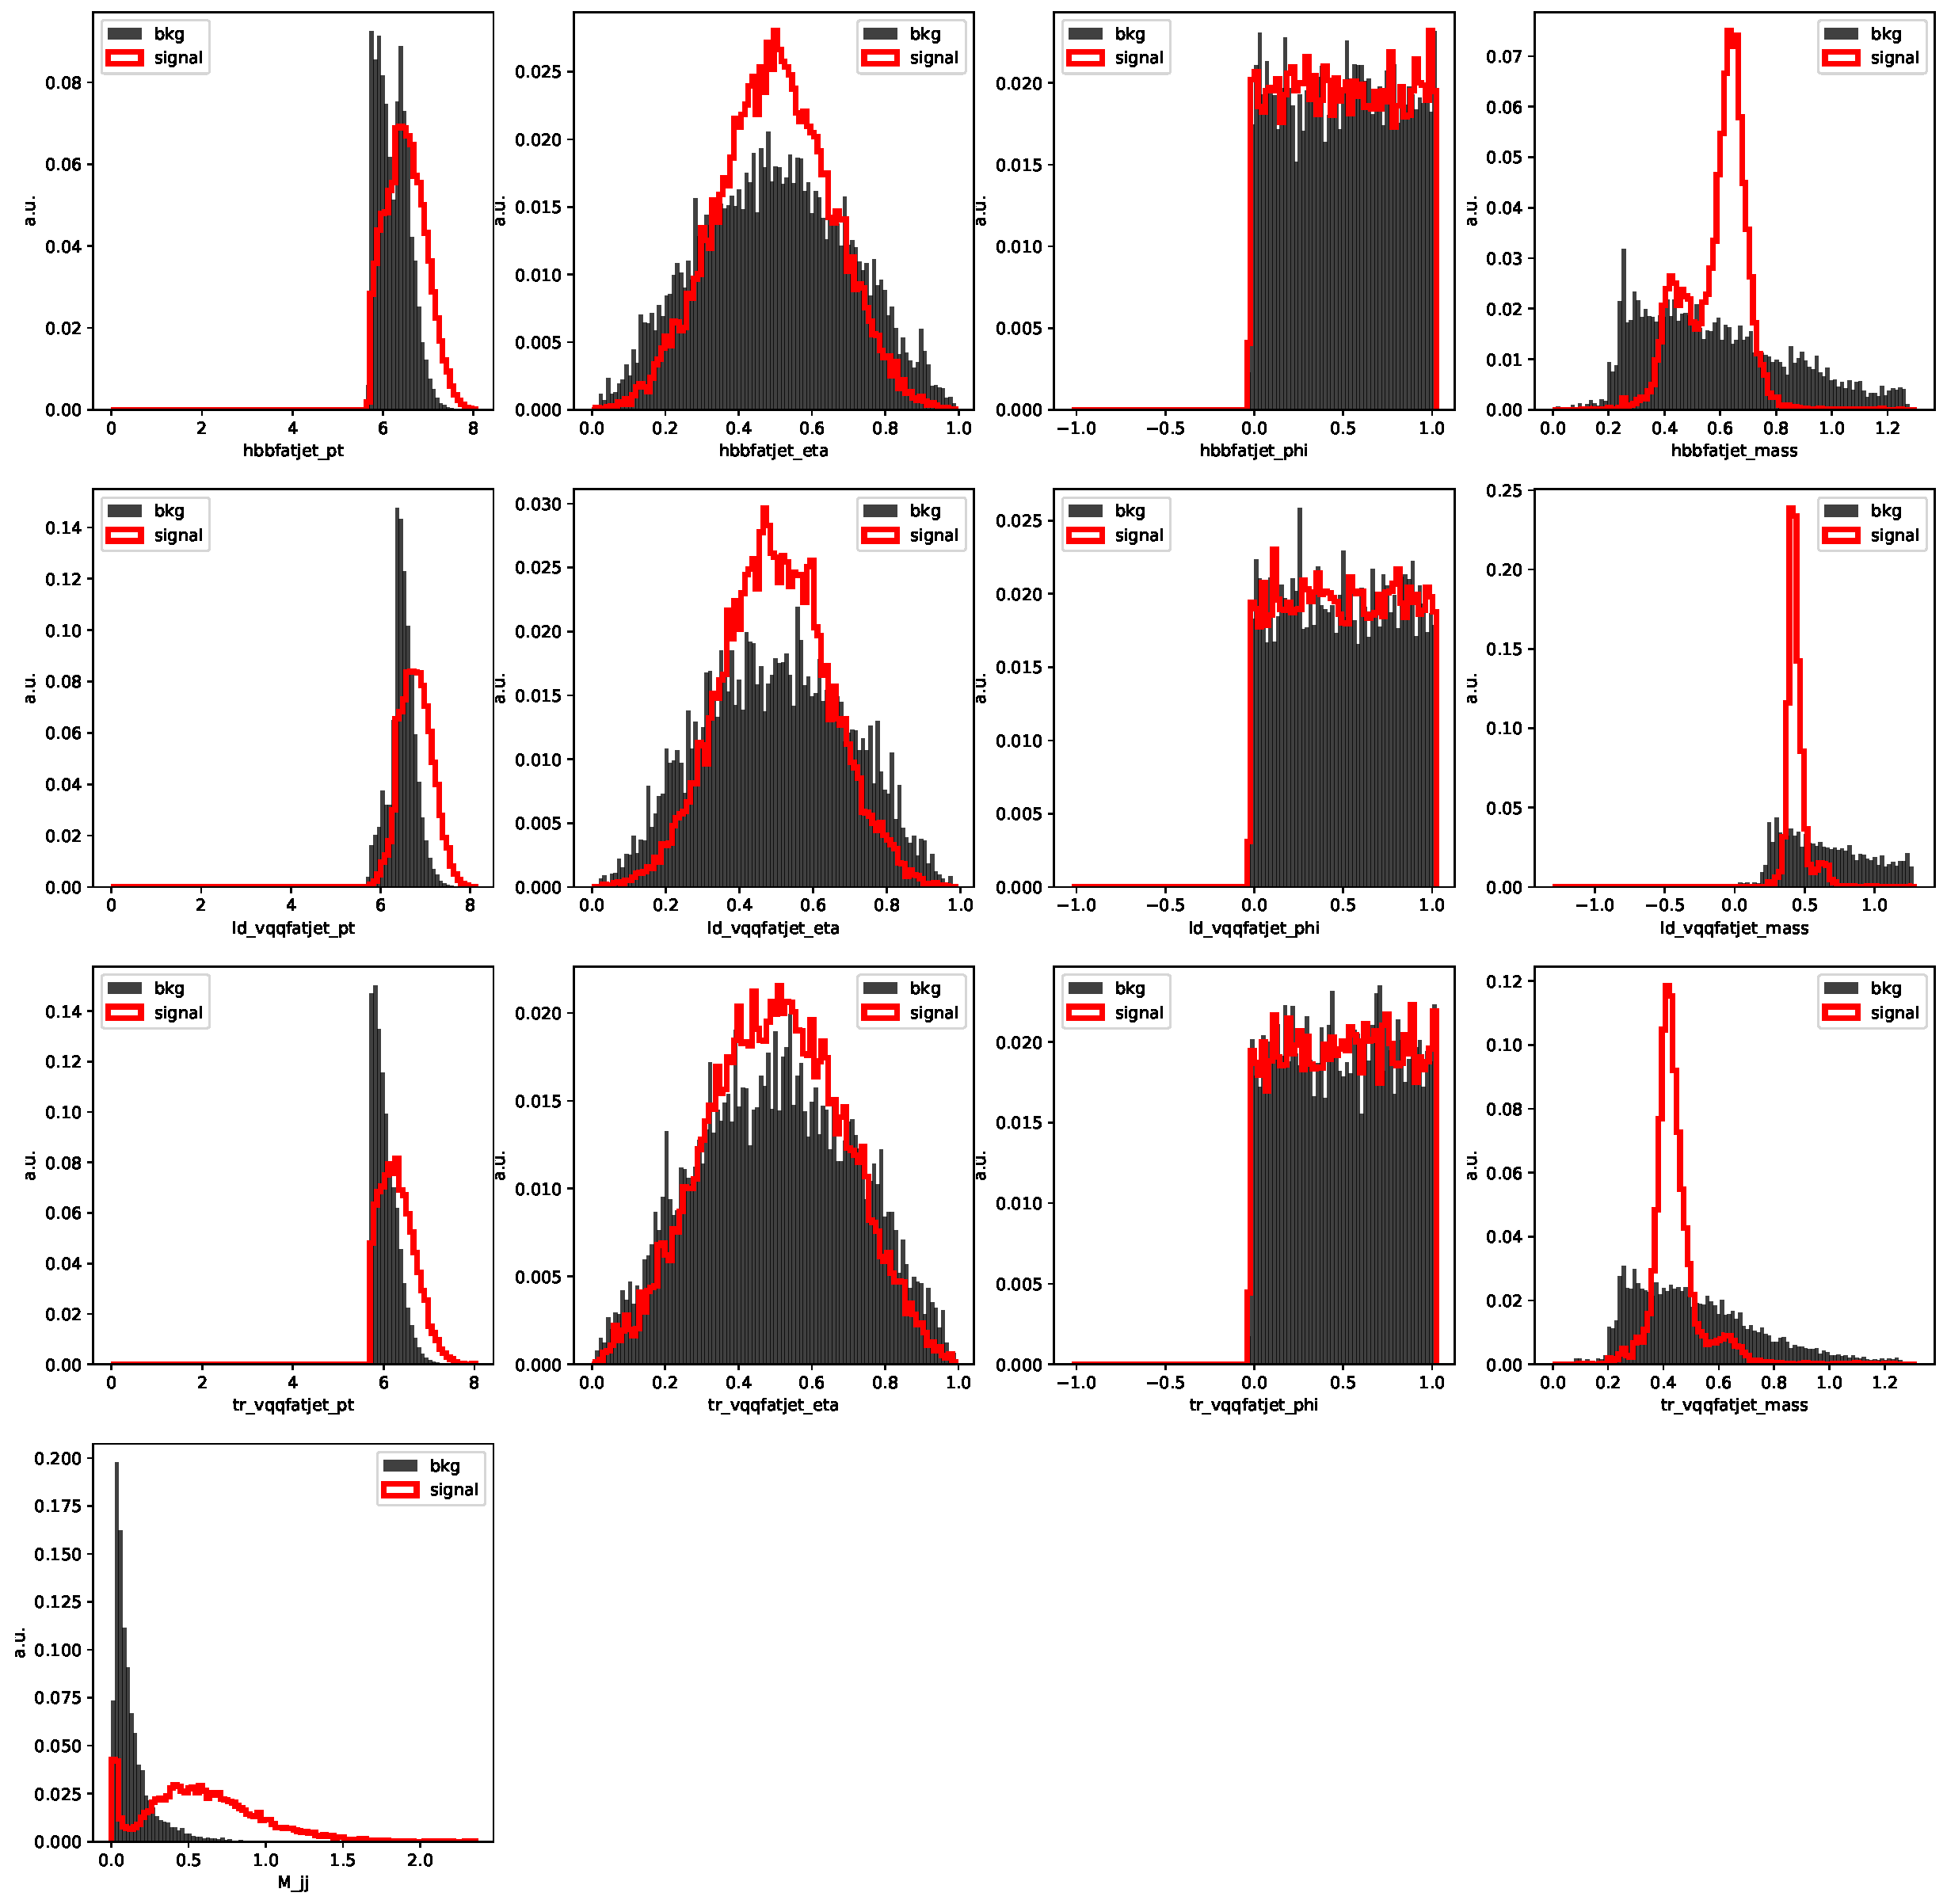
\includegraphics[width=0.75\textwidth]{fig/vbsvvh/all_features.pdf}
    \caption[The input features for \ABCDNet plotted as histograms normalized to unity]{
        The input features for \ABCDNet plotted as histograms normalized to unity. 
        It can be seen that the features have been re-scaled to values of order 1.
    }
    \label{fig:vbsvvh_abcdnet_inputs}
\end{figure}

\ABCDNet was trained for 3000 epochs with a constant learning rate. 
Once training was complete, the model was selected before the average testing and training loss start to diverge. 
Notably, the decorrelation term tends to overfit faster than BCE, and preference must be given to less overfitting in the decorrelation than in the overall performance. 
For this analysis, epoch 700 was deemed optimal (Fig.~\ref{fig:vbsvvh_abcdnet_history}).
The selected model shows no signs of overfitting and sufficient performance (Fig.~\ref{fig:vbsvvh_abcdnet_roc}). 
Moreover, it can be seen in Fig.~\ref{fig:vbsvvh_abcdnet_decorr} that the \ABCDNet discriminant (Fig.~\ref{fig:vbsvvh_abcdnet_score}) and $|\detajj|$ are indeed decorrelated.

\begin{figure}[htb]
    \centering
    \subfloat[]{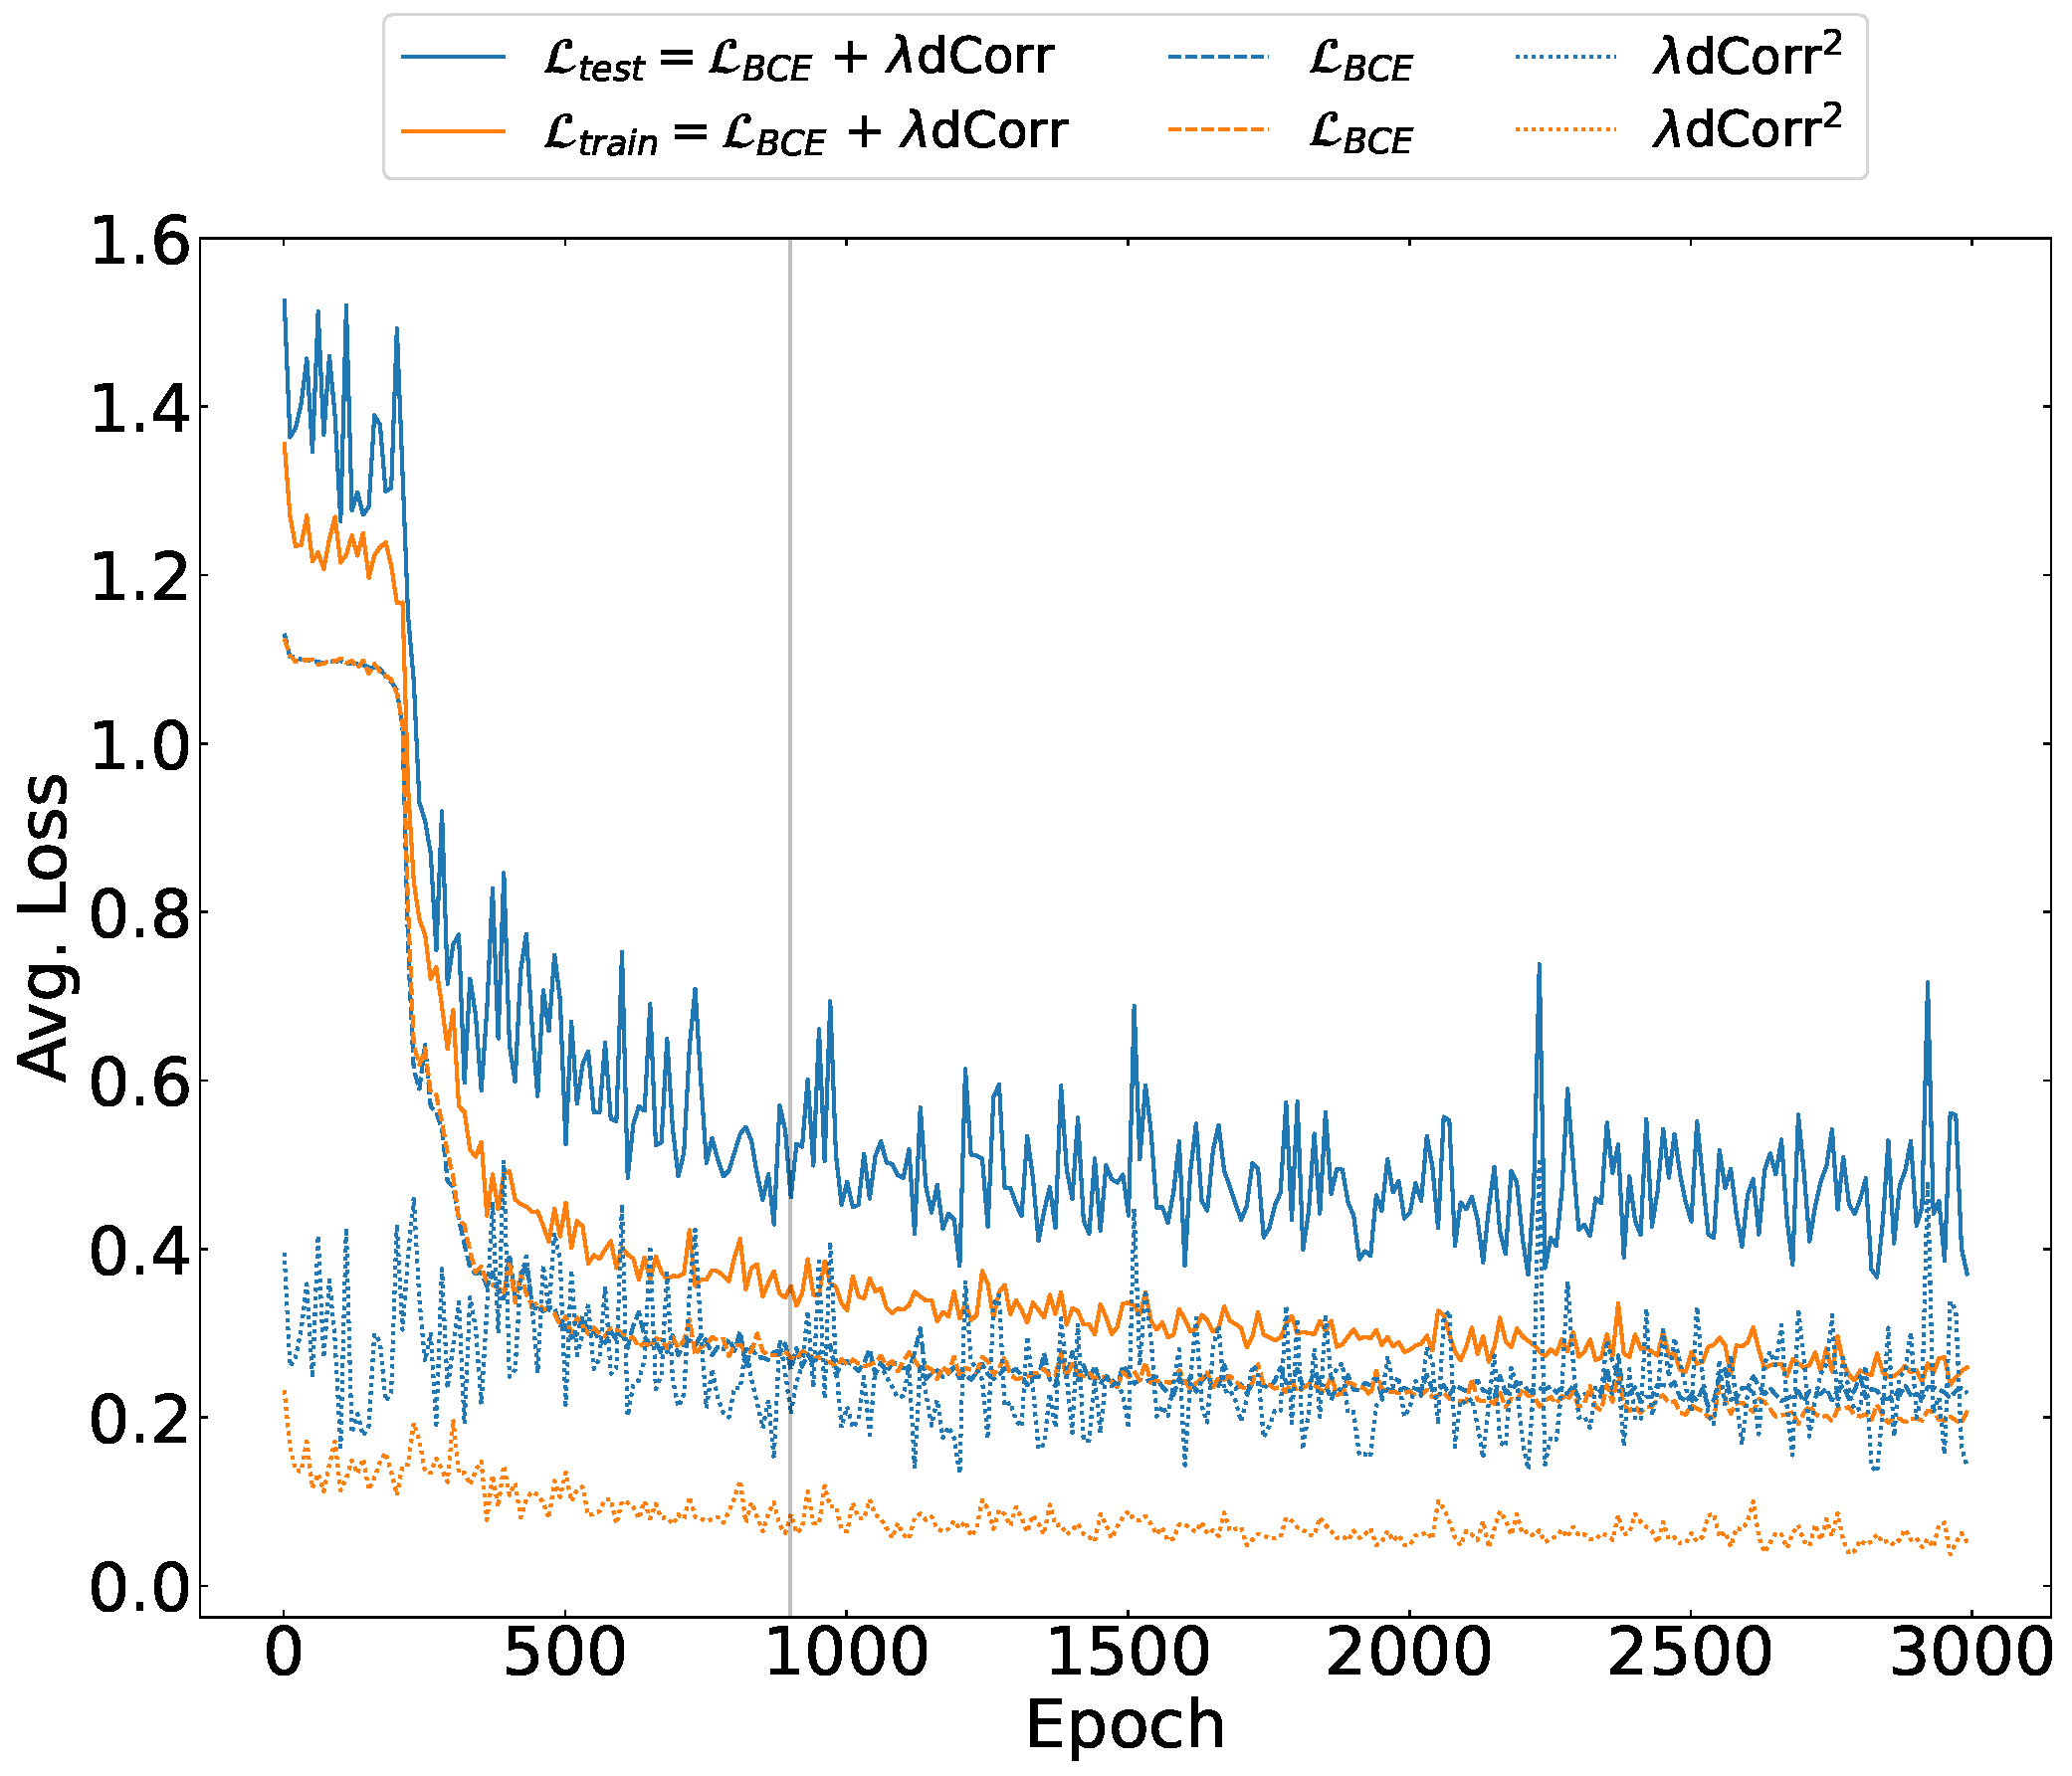
\includegraphics[width=0.5\textwidth]{fig/vbsvvh/loss_epoch900.pdf}\label{fig:vbsvvh_abcdnet_history}}
    \qquad
    \subfloat[]{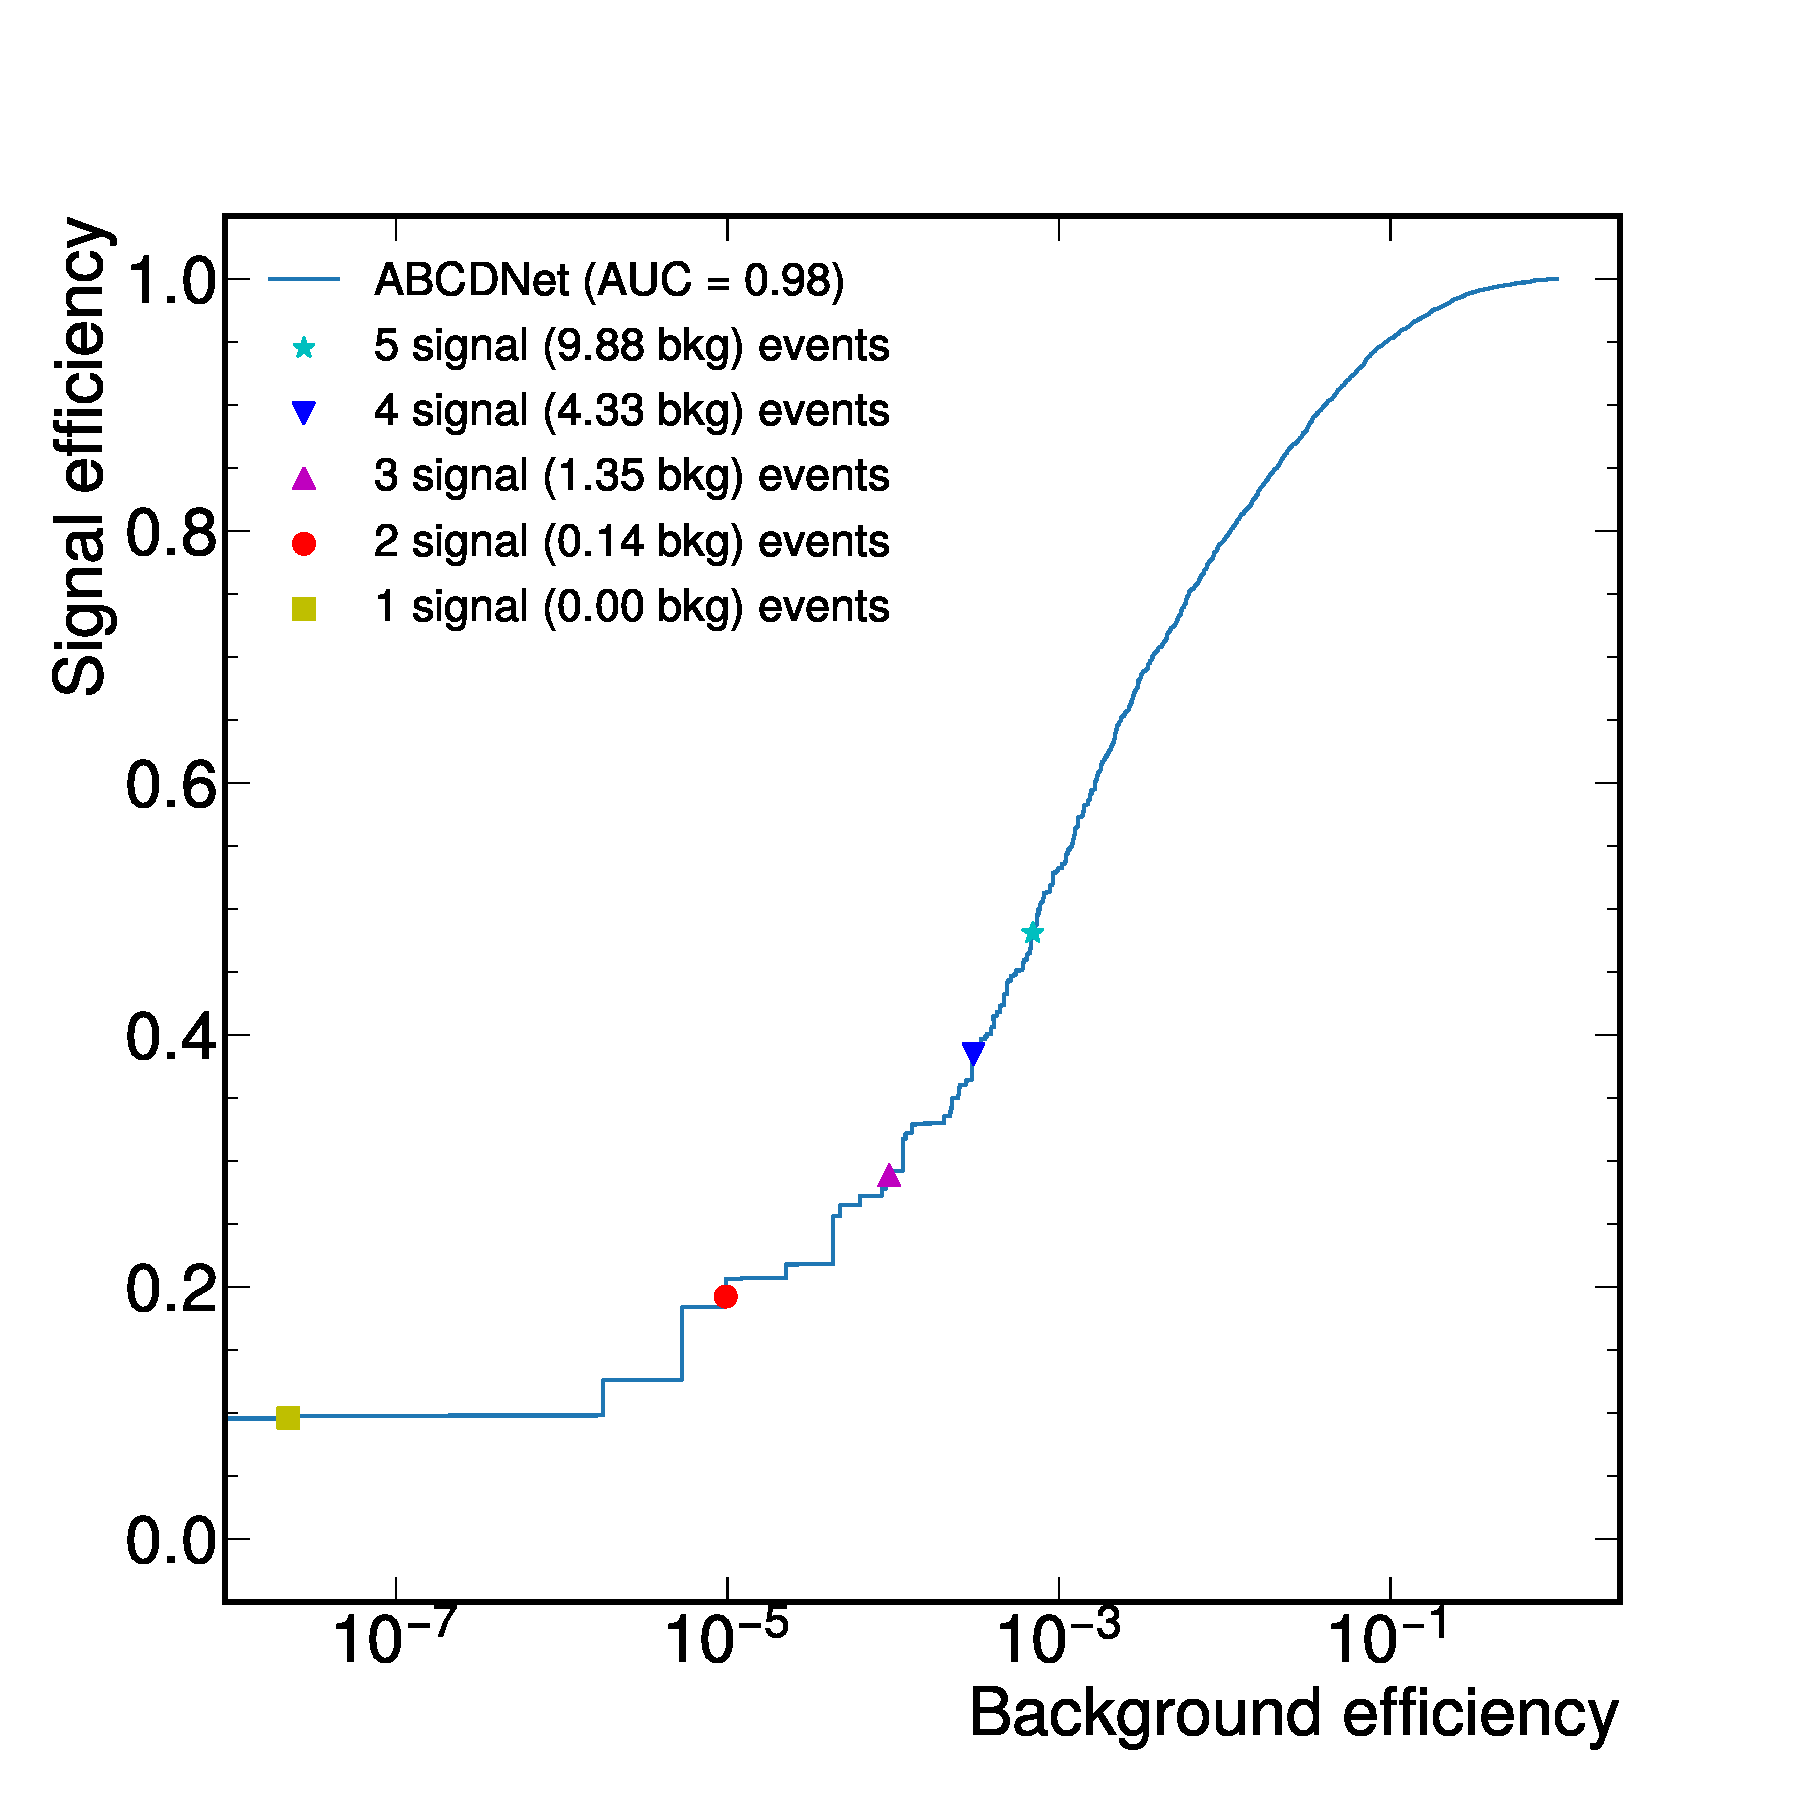
\includegraphics[width=0.4\textwidth]{fig/vbsvvh/abcdnet_roc_logx.pdf}\label{fig:vbsvvh_abcdnet_roc}}
    \caption[The average loss at each epoch and ROC curve for the selected \ABCDNet model]{
        The average loss at each epoch (left) and ROC curve for the selected model (right). 
        The total loss, which is the sum of the Binary Cross Entropy (BCE) plus the decorrelation term, is plotted as a solid line, the BCE is plotted as a dashed line, and the decorrelation term is plotted as a dotted line. 
        The testing loss is plotted in blue and the training loss is plotted in orange. 
    }
    \label{fig:vbsvvh_abcdnet_perf}
\end{figure}

\begin{figure}[htb]
    \centering
    \subfloat{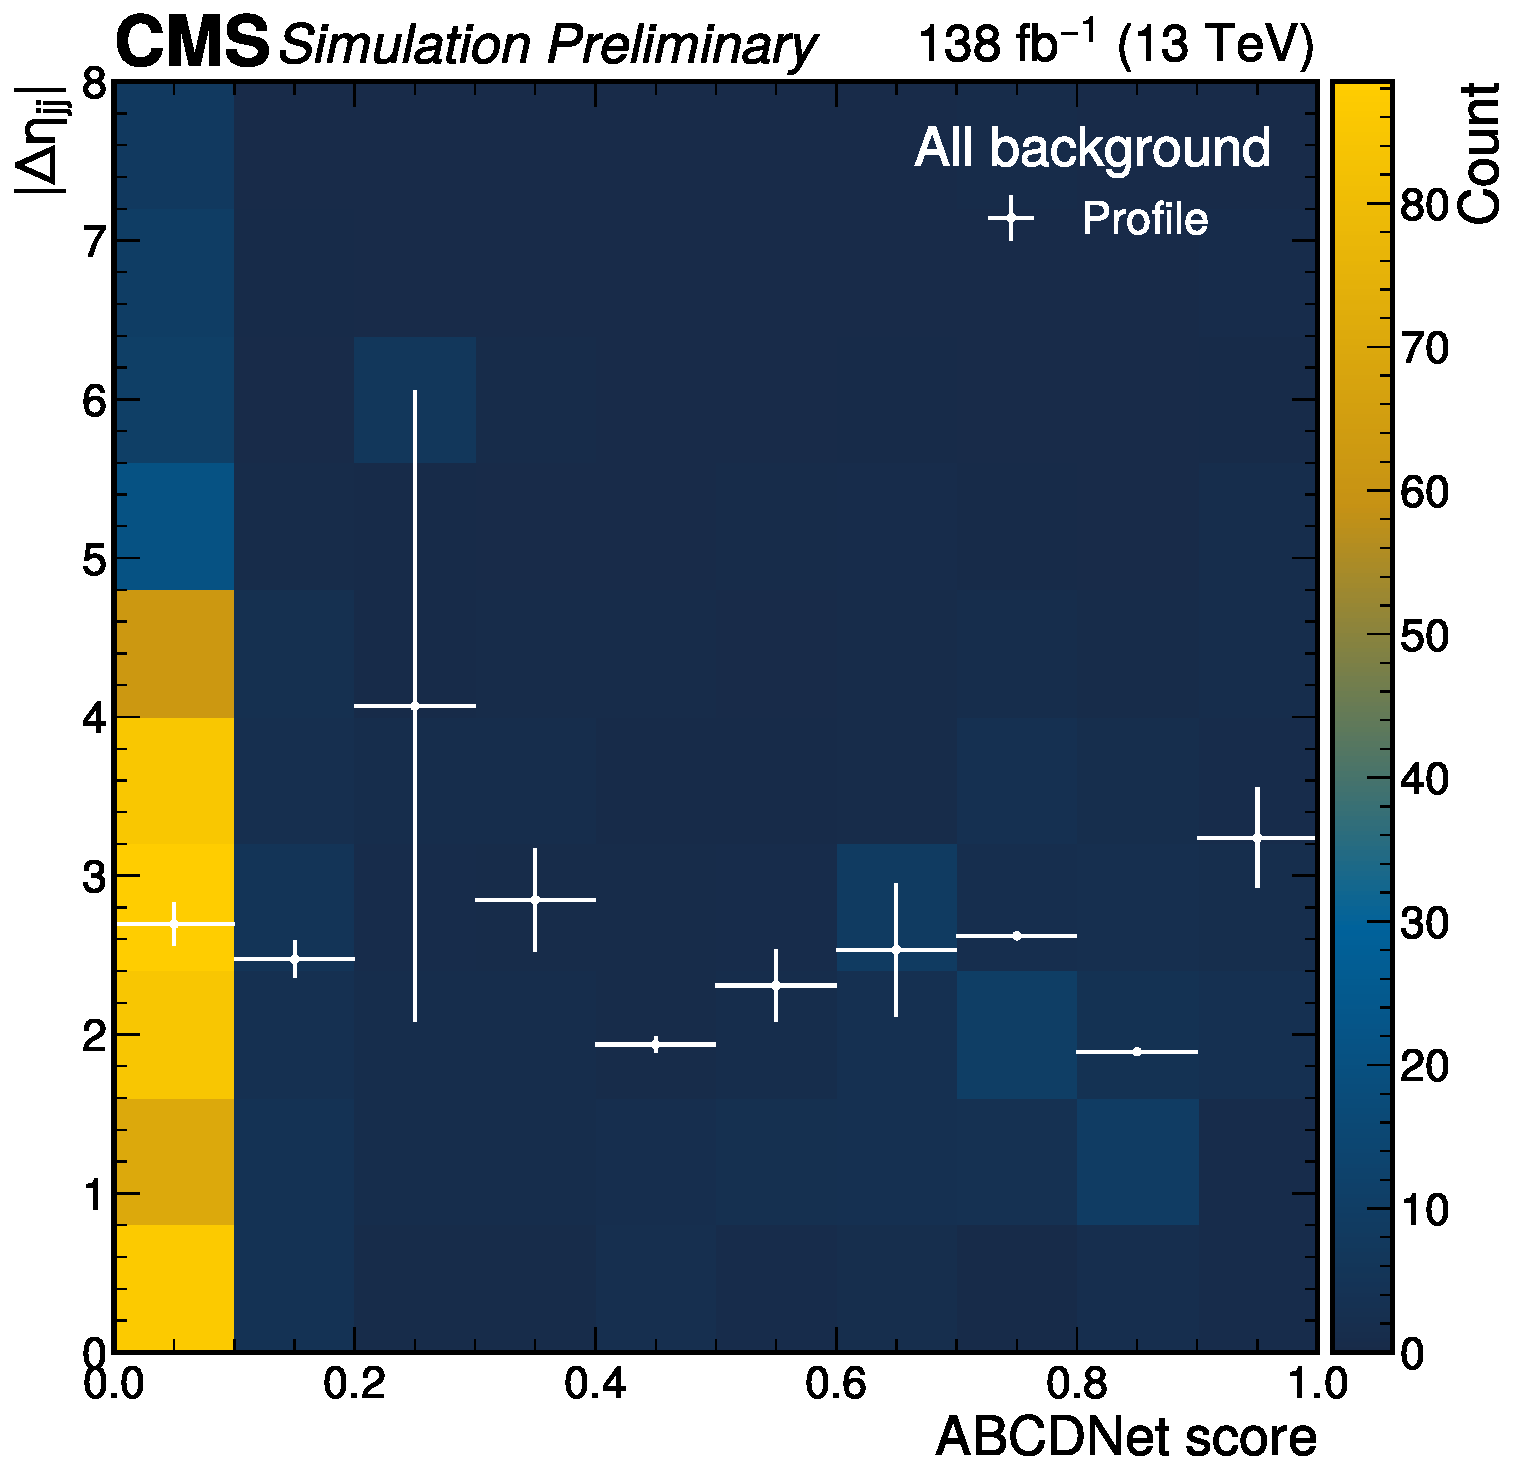
\includegraphics[width=0.45\textwidth]{fig/vbsvvh/correlation2D_abcdnet_score_abs_deta_jj_1Dprofile.pdf}}
    \qquad
    \subfloat{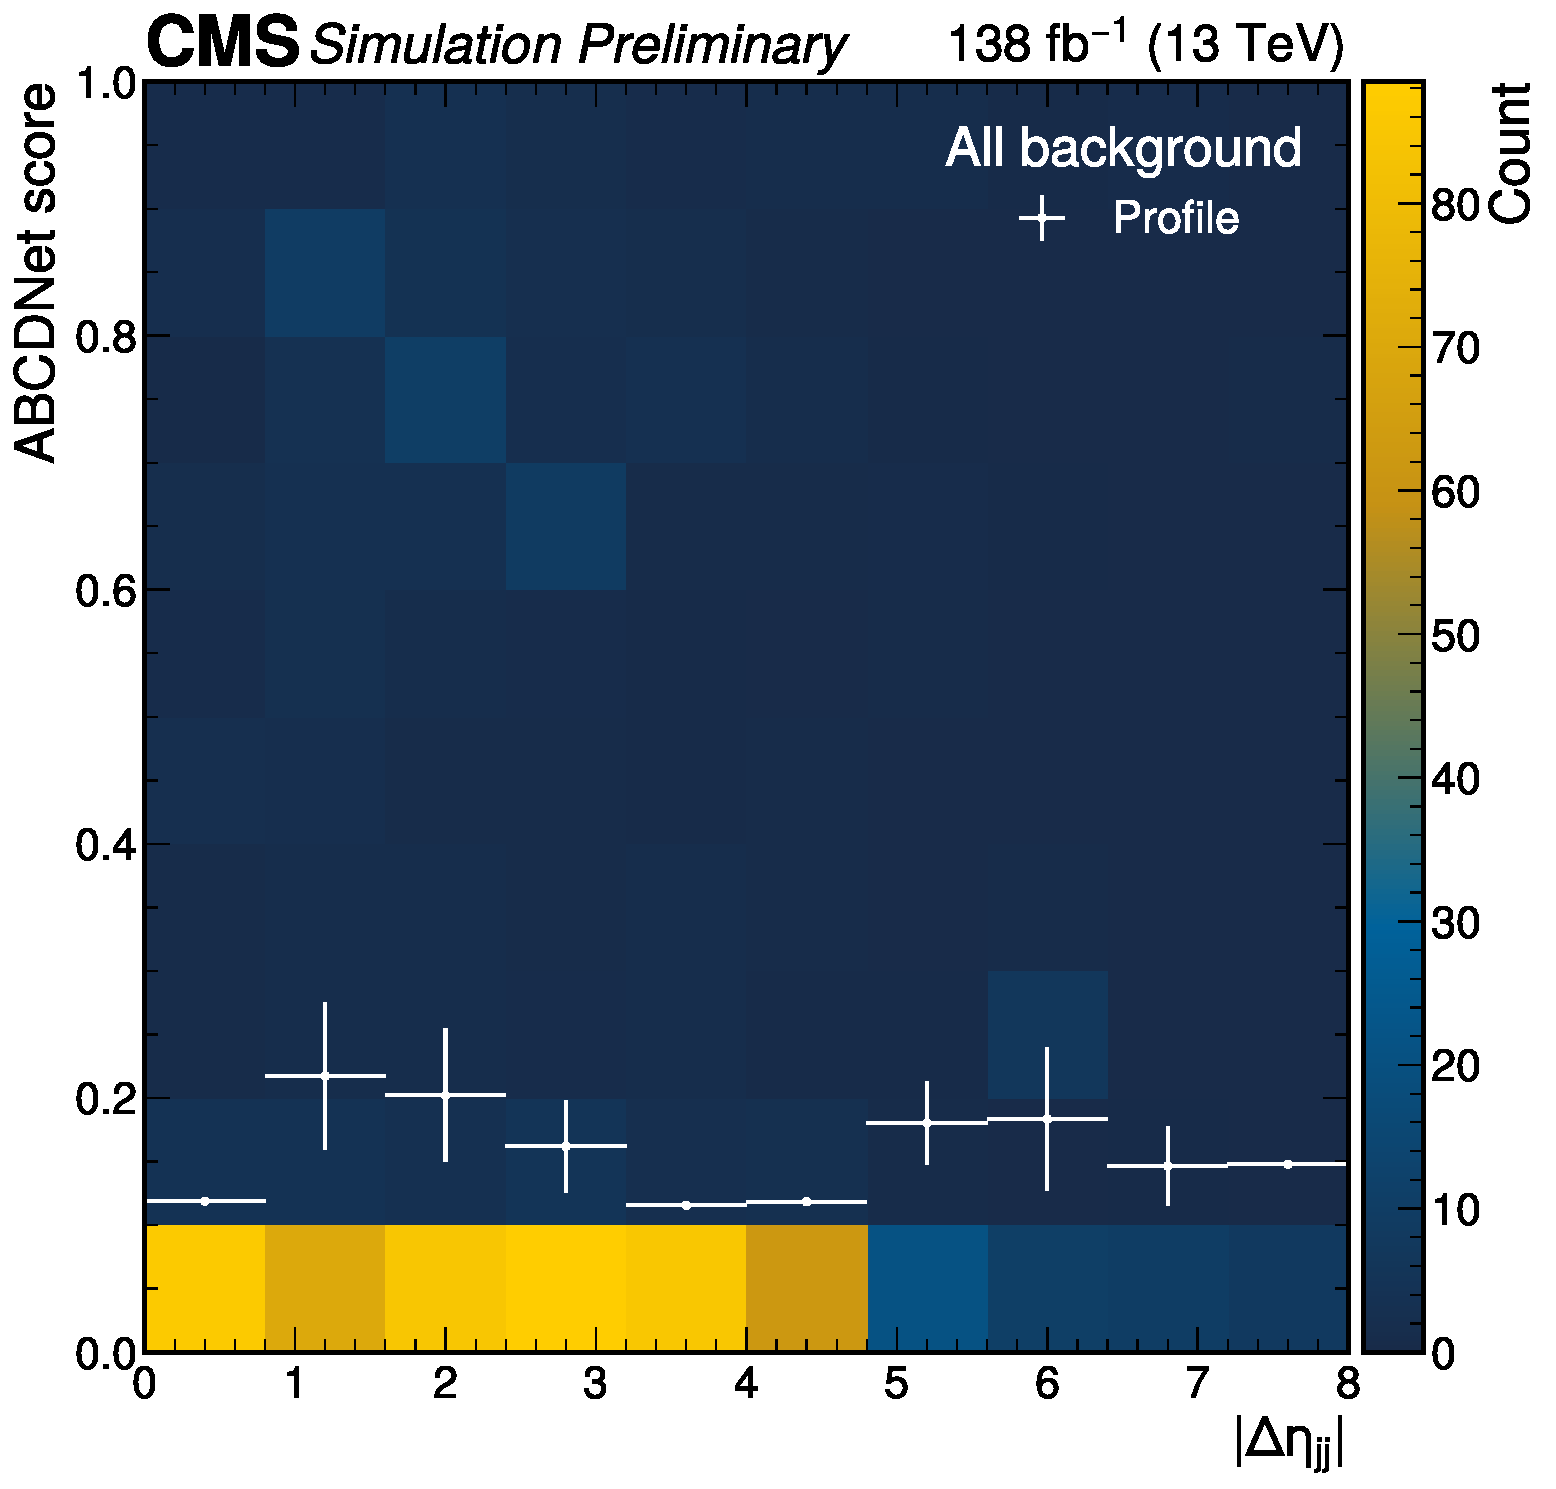
\includegraphics[width=0.45\textwidth]{fig/vbsvvh/correlation2D_abcdnet_score_abs_deta_jj_1Dprofile_flipped.pdf}}
    \caption[A two-dimensional histogram binned in \ABCDNet score and \detajj]{
        A two-dimensional histogram binned in \ABCDNet score and \detajj. 
        The one-dimensional profile of the x-axis is overlaid such that the correlation between the two variables appears as a trend in the profile. 
        The signal region selections on the AK8 jet \ParticleNet scores are applied, so the left plot is equivalent to Fig.~\ref{fig:vbsvvh_abcd}.
    }
    \label{fig:vbsvvh_abcdnet_decorr}
\end{figure}

\begin{figure}[htb]
    \centering
    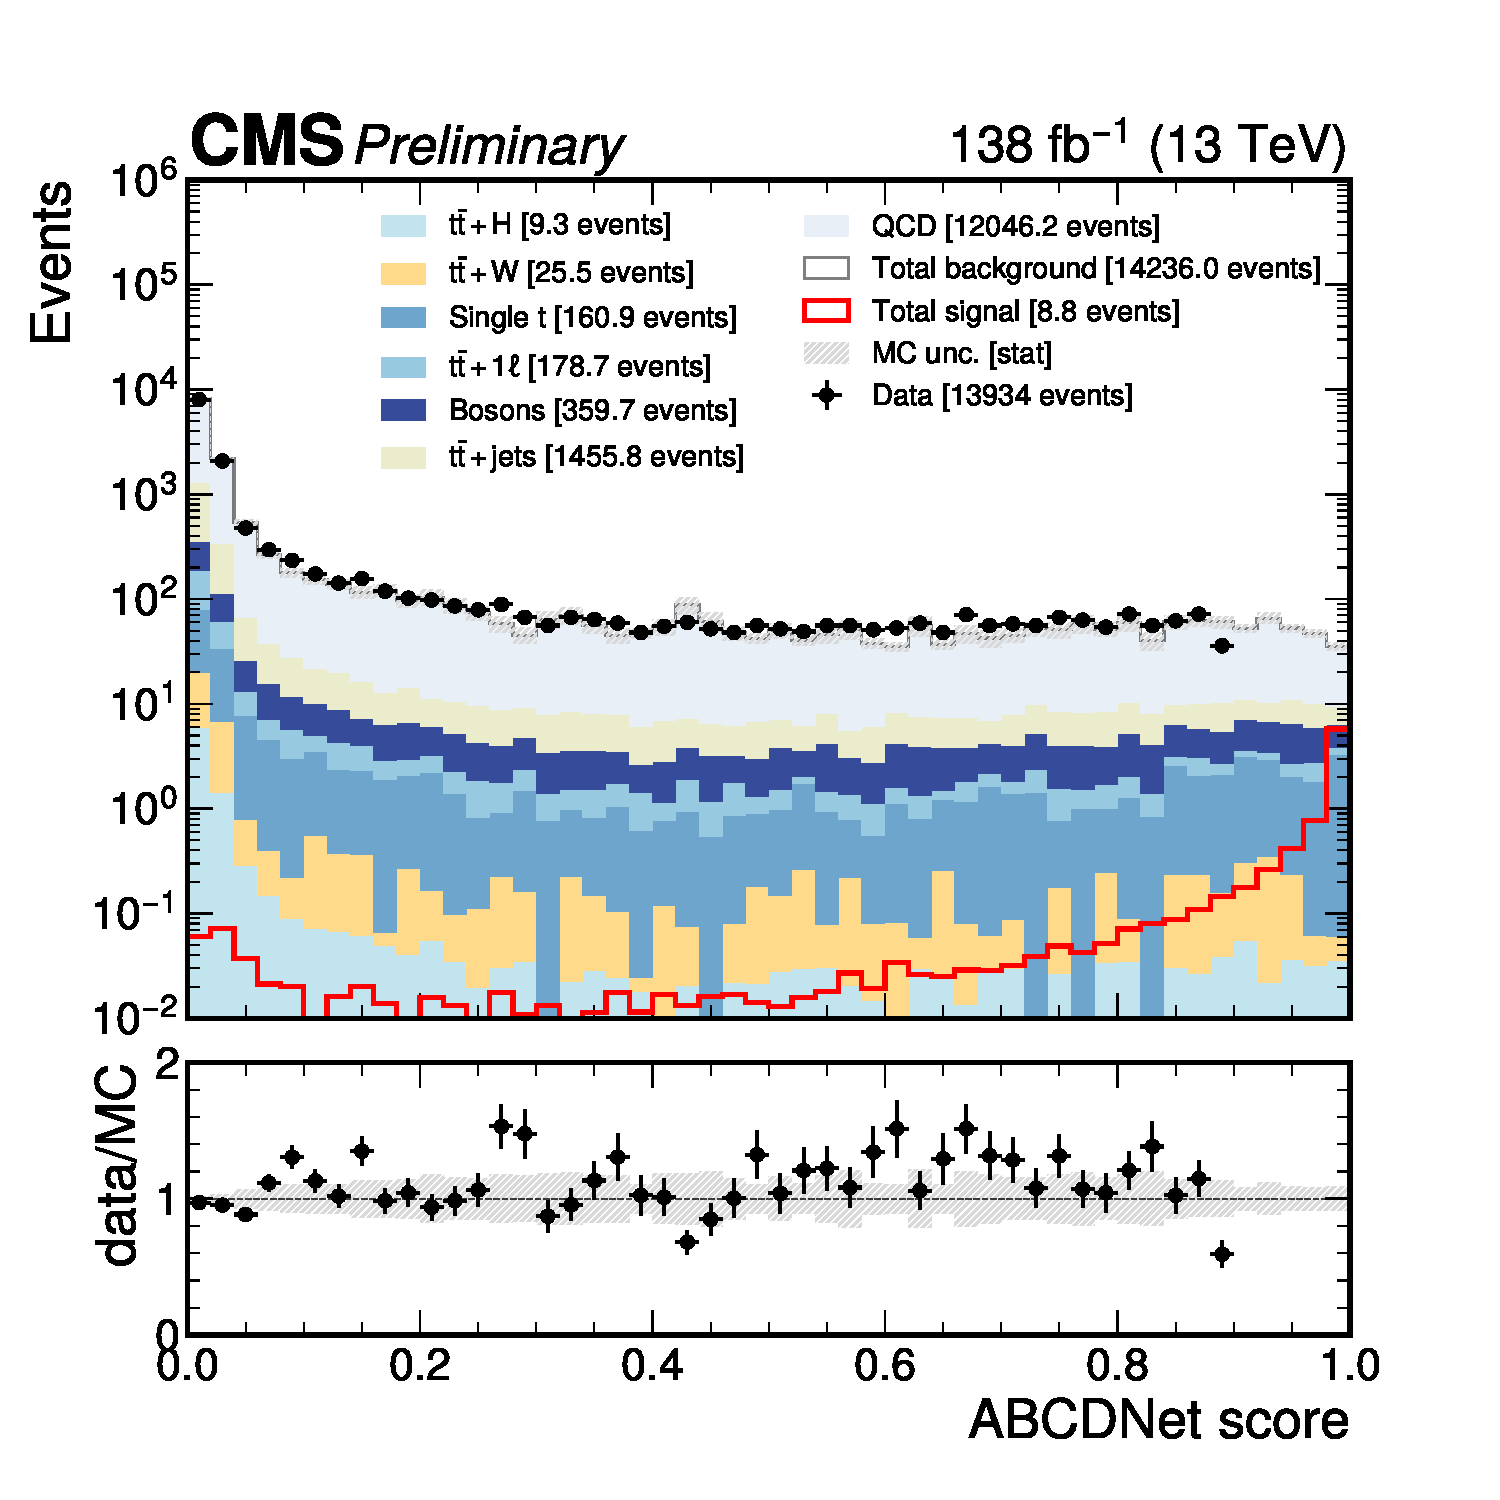
\includegraphics[width=0.45\textwidth]{fig/vbsvvh/abcdnet_score_data_vs_mc_log_presel.pdf}
    \caption[The \ABCDNet score plotted in data and MC at the Preselection]{
        The \ABCDNet score plotted in data and MC at the Preselection. 
        The data beyond the cut used in the signal region is kept blind. 
    }
    \label{fig:vbsvvh_abcdnet_score}
\end{figure}

\subsection{Signal region}
Ultimately, the signal region for this analysis is formed from cuts on five variables: \ABCDNet score, $|\detajj|$, and \ParticleNet scores for the three AK8 jets. 
A brute-force scan was performed, where over fifty thousands regions were tested. 
The regions were ranked by a rough estimation of the significance: $S/\sqrt{B}$, where $S$ is the signal yield taken from MC and $B$ is the background yield predicted using data via the ABCD method described in the next section.
The final signal region was required to have at least 0.5 predicted background events, as cutting tighter on the signal region variables resulted in larger uncertainties. 
Ultimately, the following signal region was determined:
\begin{itemize}
    \item \ABCDNet $> 0.89$
    \item $|\detajj| > 5$
    \item Xbb(\Htobb) $> 0.8$
    \item XWqq(leading \Vtoqq) $> 0.8$
    \item XWqq(trailing \Vtoqq) $> 0.7$
\end{itemize}

\section{Background estimation}
The background in the signal region is estimated entirely from data by using the ``ABCD'' method, where regions A, B, C, and D are illustrated in Fig.~\ref{fig:vbsvvh_abcd}. % and Fig.~\ref{fig:vbsvvh_abcdFlowchart}. 
These regions are formed by selecting two cuts in the signal region (region A), then inverting them to form regions B, C, and D. 
So long as the two cuts are independent, the following method holds. 
As in the previous analysis, the background yield in regions A, B, C, and D in Monte Carlo are defined as \AMC, \BMC, \CMC, and \DMC.
Likewise, let the same yields in data be defined as  \Adata, \Bdata, \Cdata, and \Ddata.
Again, the estimated background yield in the signal region \AdataPred can be computed using Eq.~\ref{eq:vbswh_abcd}, reproduced here for convenience:
\begin{equation*}
    \AdataPred = \Bdata\times\frac{\Cdata}{\Ddata}
\end{equation*}
where the same can be done in MC, yielding \AMCPred. 
The two cuts used to define the ABCD method are \ABCDNet $> 0.89$ and $|\detajj| > 5$. 
Because \ABCDNet was trained to be decorrelated with \detajj, the method holds by construction. 
Now, it can be seen in Fig.~\ref{fig:vbsvvh_abcd_closureMass} that data and MC agree reasonably well in regions A, B, and C. 
The statistical uncertainty \Estat on the method is simply the propagation of statistical uncertainties on the data yields for regions B, C, and D:
\begin{equation}\label{eq:vbsvvh_statUnc}
    \Estat = \frac{\sqrt{\Bdata}}{\Bdata} \oplus \frac{\sqrt{\Cdata}}{\Cdata} \oplus \frac{\sqrt{\Ddata}}{\Ddata} \approx 34\% 
\end{equation}

\begin{figure}[htb]
    \centering
    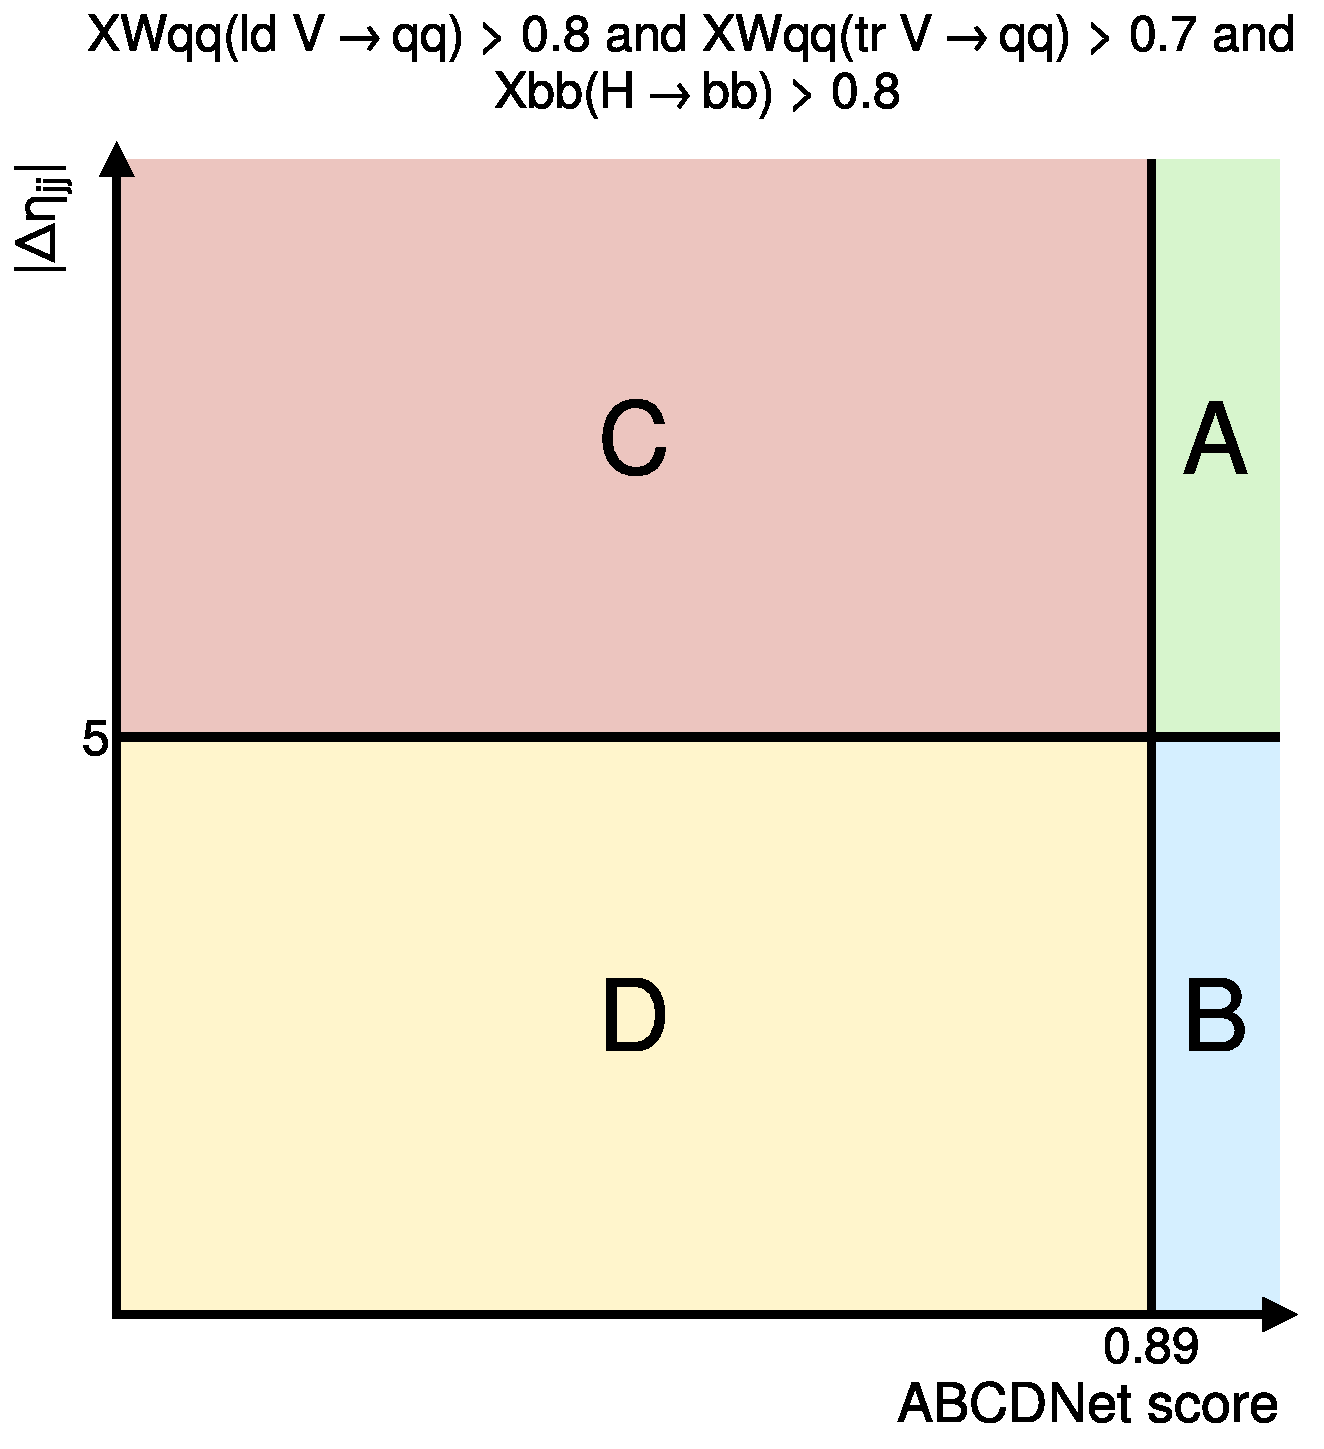
\includegraphics[width=0.45\textwidth]{fig/vbsvvh/ABCD_abcdnet_score_gt_0p89_vs_abs_deta_jj_gt_5p0.pdf}
    \caption[A cartoon of the ABCD regions]{
        A cartoon of the ABCD regions. 
        The signal region selections on the AK8 jet \ParticleNet scores are applied to all regions. 
        Region B has the \detajj cut inverted, region C has the \ABCDNet score inverted, and region D has both cuts inverted. 
    }
    \label{fig:vbsvvh_abcd}
\end{figure}

\begin{table}[htbp]
    \centering
    \caption[VBS $\VVH$ ABCD yields]{
        Data yields and region A prediction for the control region used for the ABCD closure test. 
        The region A yield is kept blind, while $A_{pred}$ is reported.
    }
    \begin{tabular}{ccc}
    \toprule
    \textbf{Region} & Data Yield & Prediction \\
    \midrule
    A               & --         & 1.07       \\
    B               & 10         &            \\
    C               & 72         &            \\
    D               & 672        &            \\
    \bottomrule
    \end{tabular}
    \label{tab:0lepABCDregion}
\end{table}

We can immediately assess the closure of the method using only simulated events by comparing \AMCPred and \AMC:
\begin{equation*}
    \AMCPred = \BMC\times\frac{\CMC}{\DMC} = 1.12\pm0.29 \qquad \AMC = 2.34\pm0.82
\end{equation*}
However, the conclusion from this test is not clear, given the large uncertainty on the MC prediction in region A. 
Instead, a systematic uncertainty on the method \Esyst can be derived using MC as follows:
\begin{equation}
    \Esyst = 
        \frac{2}{\AMC + \AMCPred}
        \sqrt{\bigg(\frac{\AMC^\text{err}}{\AMC}\bigg)^2 + \bigg(\frac{\Estat^\mathrm{MC}}{\AMCPred}\bigg)^2} \approx 25\%
\end{equation}
This effectively takes the relative error on the non-closure in MC as the systematic uncertainty, where $\AMC^\text{err}$ is the statistical error on the MC yield and $\Estat^\mathrm{MC}$ is the equivalent of Eq.~\ref{eq:vbsvvh_statUnc} for MC.

\begin{figure}[htb]
    \centering
    \subfloat[]{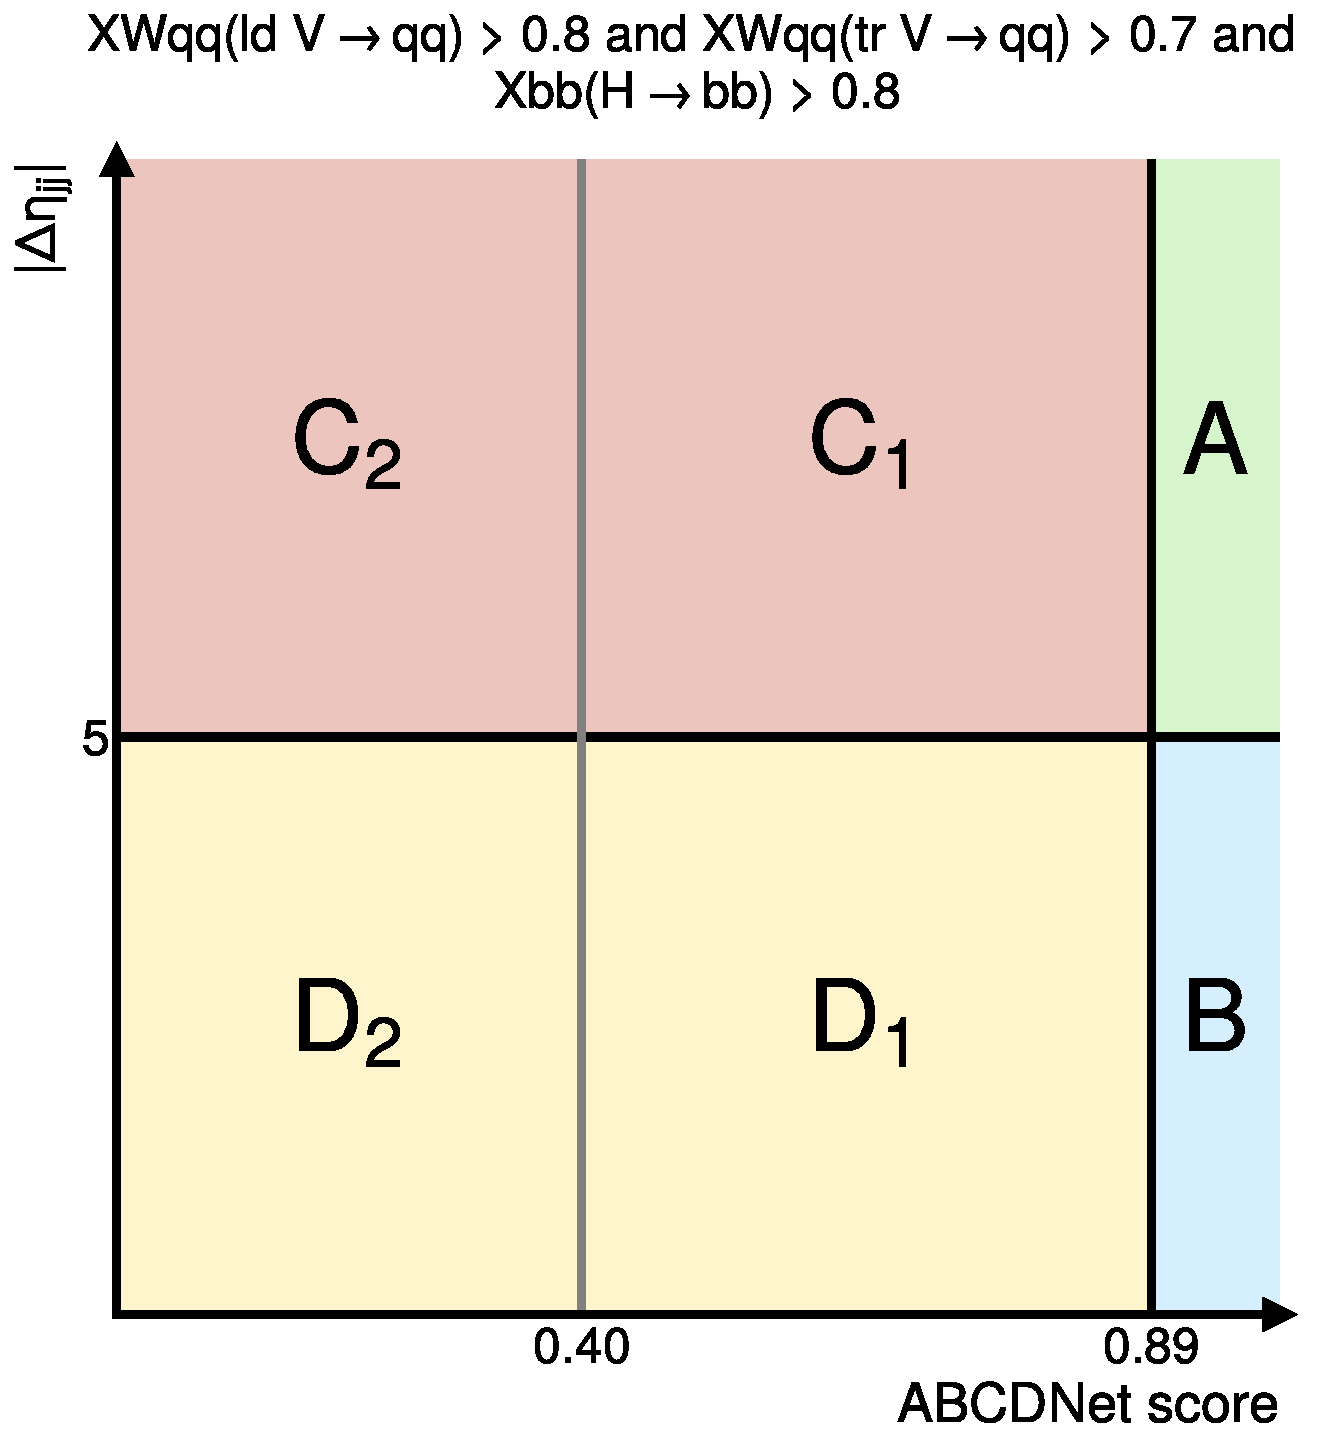
\includegraphics[width=0.45\textwidth]{fig/vbsvvh/ABC1C2D1D2_abcdnet_score_gt_0p89_vs_abs_deta_jj_gt_5p0.pdf}\label{fig:vbsvvh_abcdCheck1}}
    \qquad
    \subfloat[]{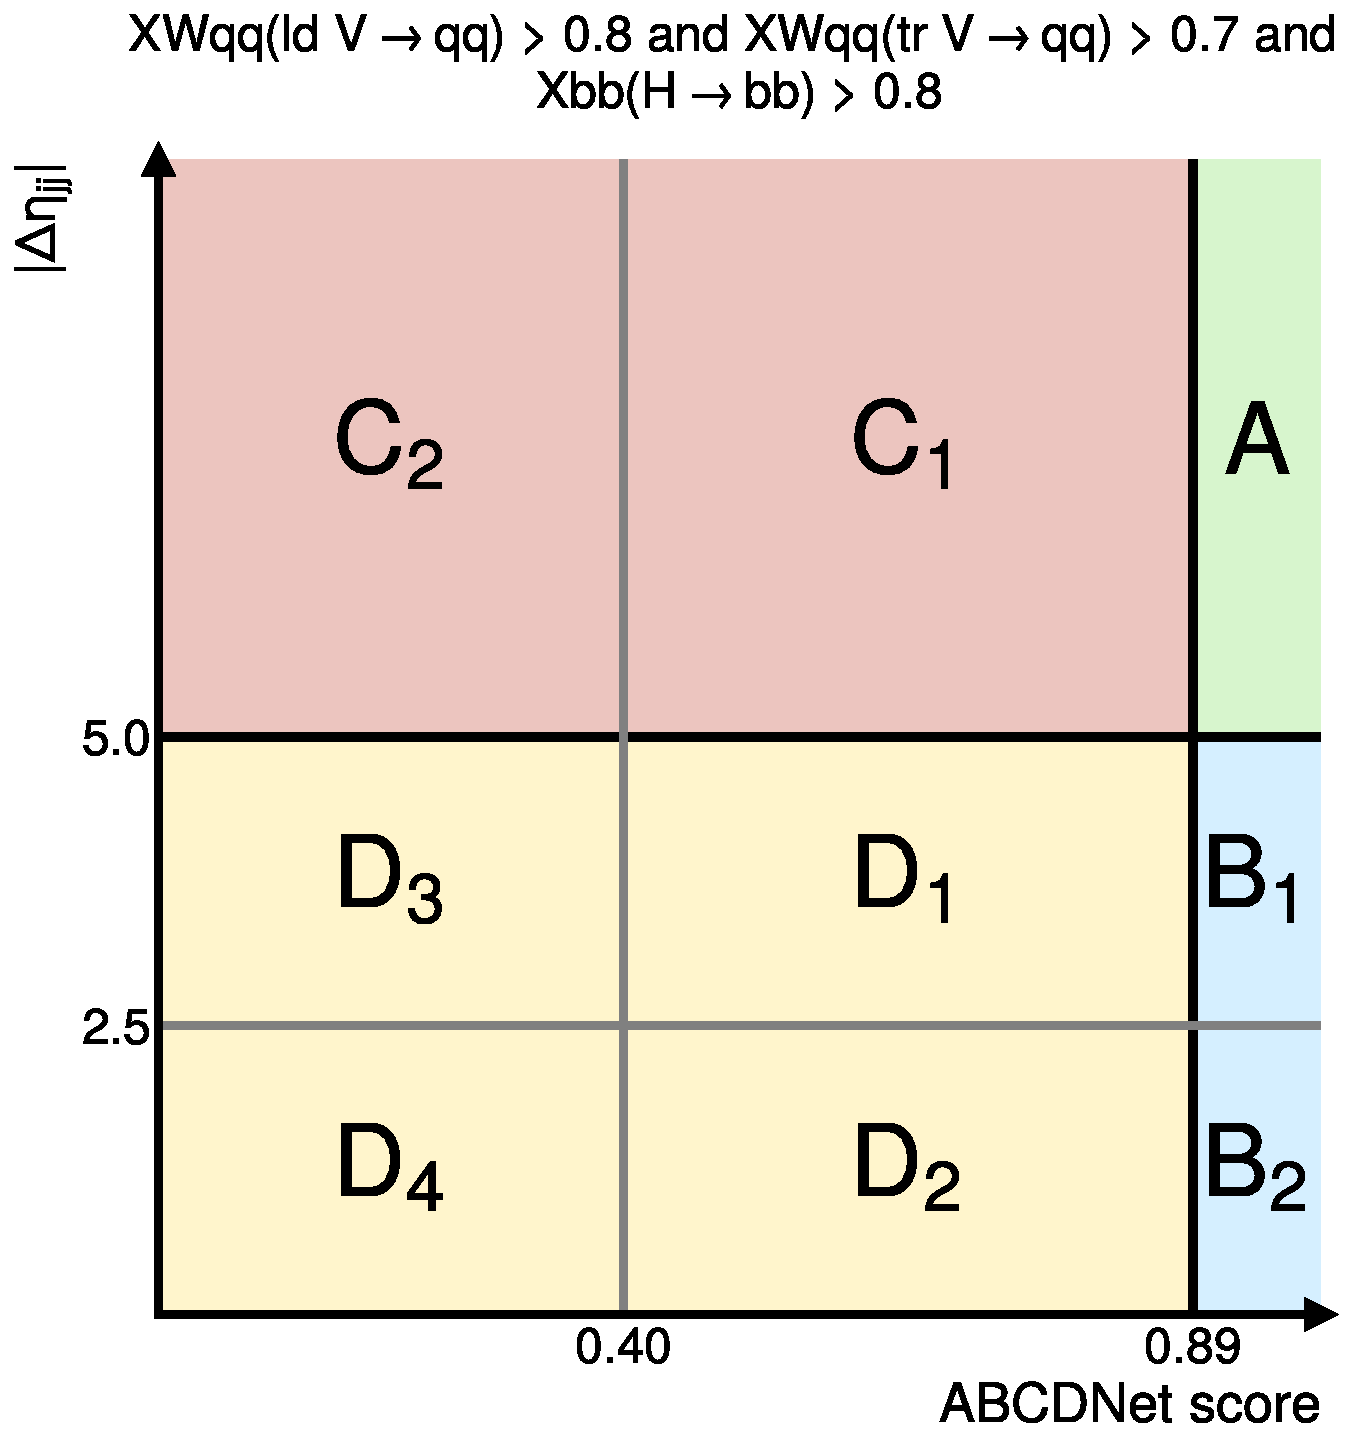
\includegraphics[width=0.45\textwidth]{fig/vbsvvh/AB1B2C1C2D1D2_abcdnet_score_gt_0p89_vs_abs_deta_jj_gt_5p0.pdf}\label{fig:vbsvvh_abcdCheck2}}
    \caption[The ABCD regions used for closure tests]{
        The ABCD regions used for closure tests. 
        Again, the cuts on the AK8 jet \ParticleNet scores are applied to all regions. 
        Regions C and D can each be split into two sub-regions by introducing a looser cut on the \ABCDNet score (a). 
        Region B can similarly be split into two sub-regions by introducing a looser cut on \detajj, which also divides D into 4 sub-regions total (b).
    }
    \label{fig:vbsvvh_abcd_extra}
\end{figure}

\begin{figure}[htb]
    \centering
    \subfloat{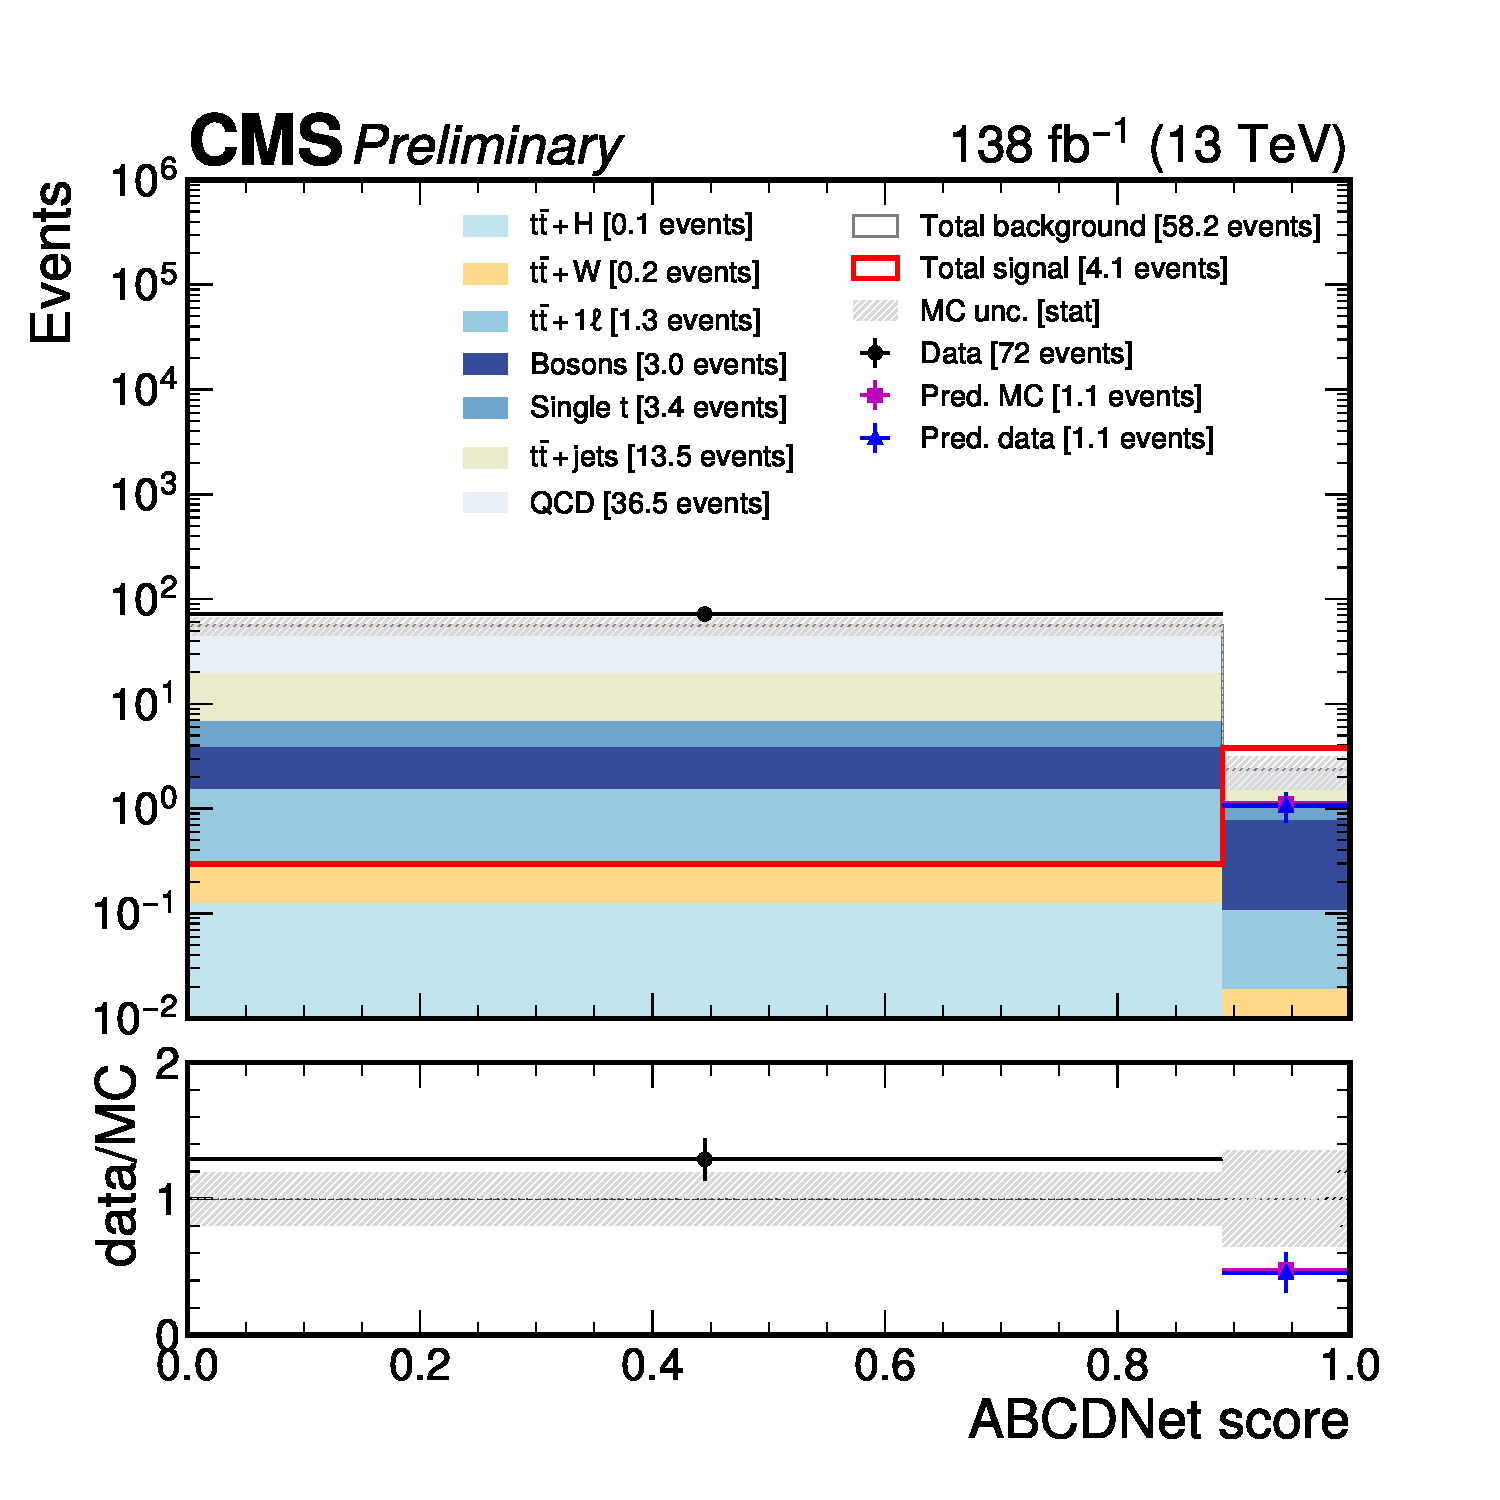
\includegraphics[width=0.45\textwidth]{fig/vbsvvh/regionsAC_closure_signal.pdf}}
    \qquad
    \subfloat{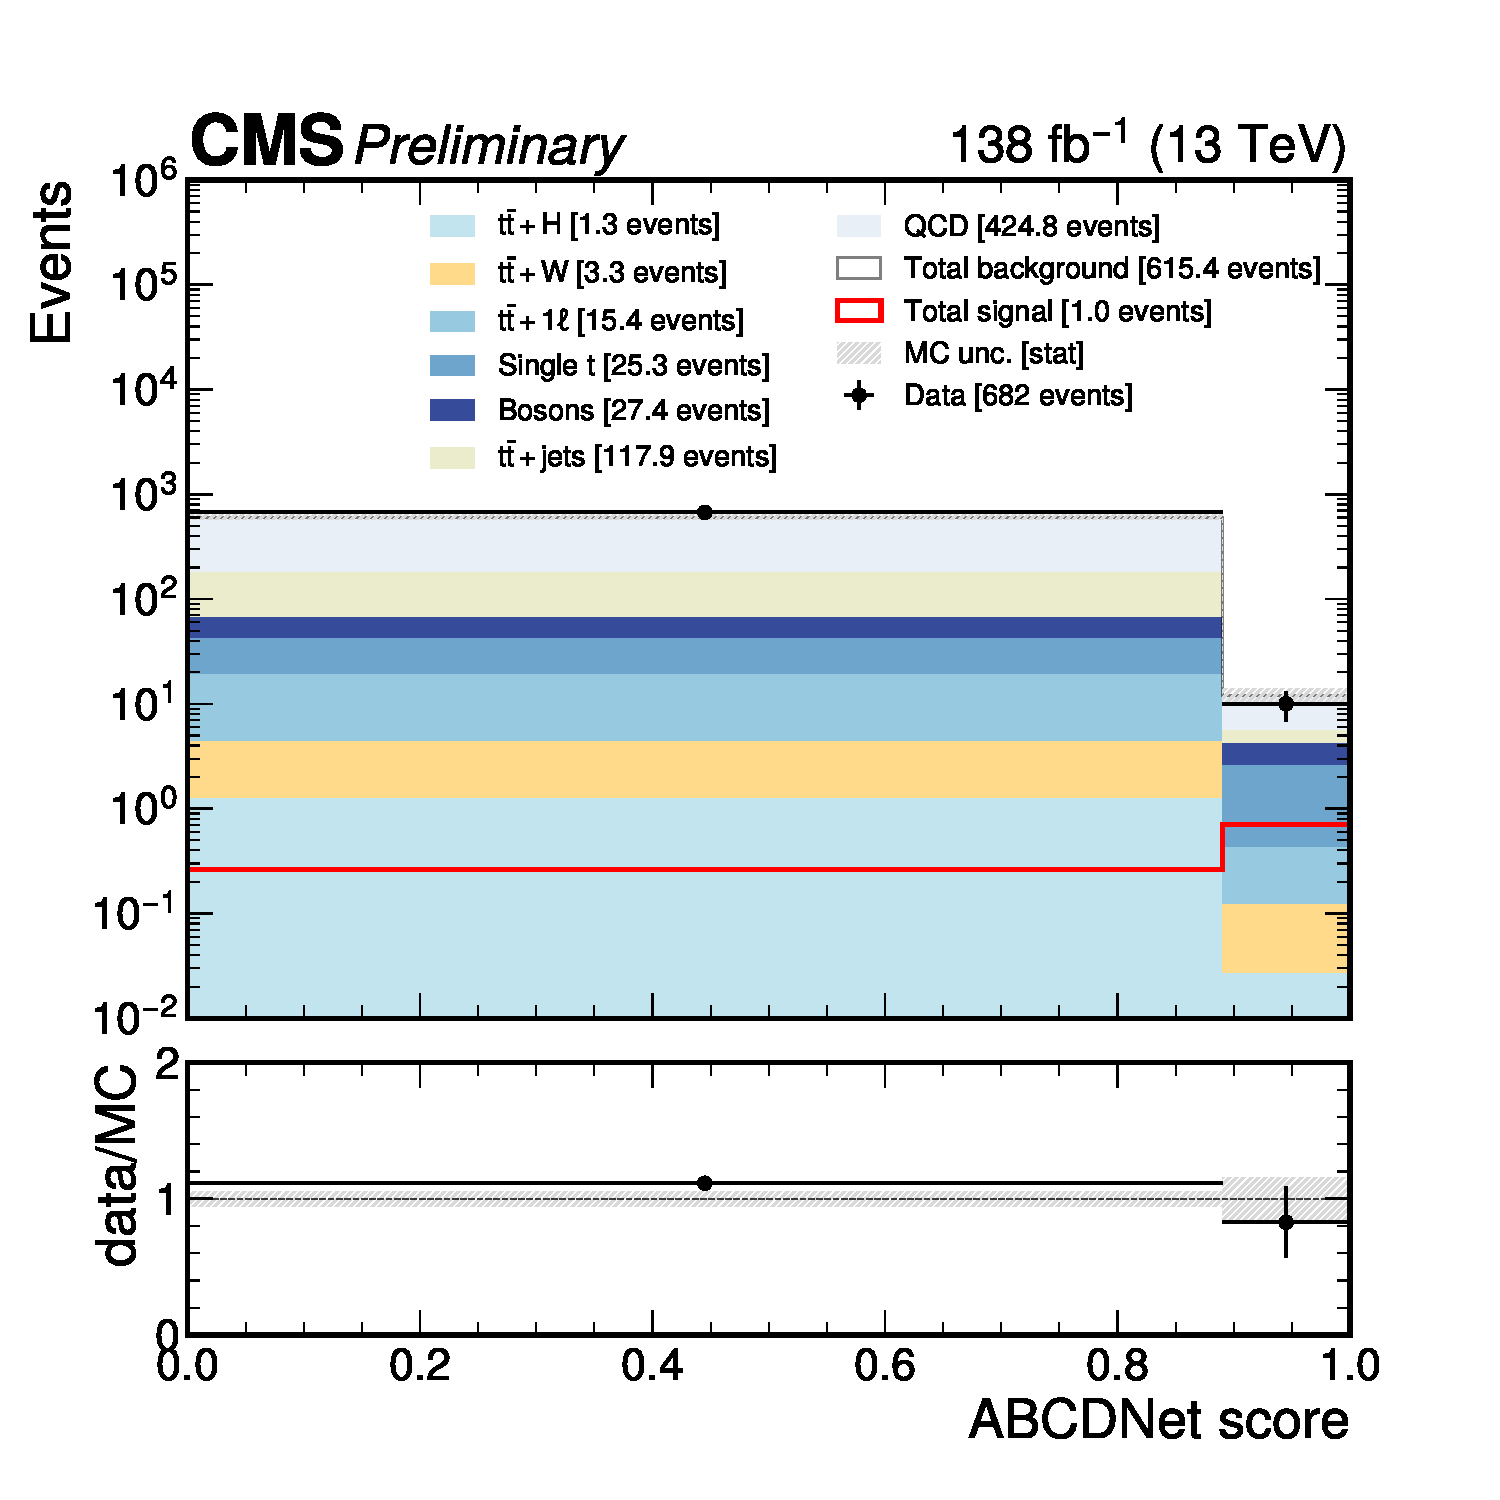
\includegraphics[width=0.45\textwidth]{fig/vbsvvh/regionsBD_closure_signal.pdf}}
    \caption[Regions A, B, C, and D used in the ABCD method]{
        Regions A and C (left) and regions B and D (right) used in the ABCD method.
    }
    \label{fig:vbsvvh_abcd_closureMass}
\end{figure}

Ultimately, the ABCD method will be applied exclusively in data, so showing good closure only in MC would not fully ensure the validity of the method in data. 
Moreover, the MC statistics are limited in the signal region, so the exact quality of the closure is not clear from MC alone. 
In order to verify that the method is valid in data, the sidebands B, C, and D can be divided into sub-regions as shown in Fig.~\ref{fig:vbsvvh_abcdCheck2}. 
The ABCD method should still hold in these sub-regions, and because regions B, C, and D exclude the signal region, closure can be evaluated in data. 
In total, 5 such checks are done, and the results are tabulated in Table~\ref{tab:vbsvvh_closureTests}. 
In each test, good closure is seen in data, supporting the validity of the method.

\begin{table}[htbp]
    \centering
    \caption[VBS $\VVH$ ABCD cross-check yields]{
        Data yields and signal-like region prediction for the ABCD closure tests. 
        Regions B$_i$, C$_i$, and D$_i$ are described in Fig.~\ref{fig:vbsvvh_abcd_extra}.
    }
    \subfloat{
        \begin{tabular}{ccc}
        \toprule
        \textbf{Region} & Data Yield    & Prediction    \\
        \midrule
        B$_1$           & $  3\pm1.7 $ & $ 5.6\pm2.5 $ \\
        B$_2$           & $  7\pm2.7 $ &               \\
        D$_1$           & $ 27\pm5.2 $ &               \\
        D$_2$           & $ 34\pm5.8 $ &               \\
        \bottomrule
        \end{tabular}
    }
    \subfloat{
        \begin{tabular}{ccc}
        \toprule
        \textbf{Region} & Data Yield    & Prediction    \\
        \midrule
        D$_1$           & $  27\pm5.2 $ & $ 24\pm4.6 $  \\
        D$_2$           & $  34\pm5.8 $ &               \\
        D$_3$           & $ 255\pm16  $ &               \\
        D$_4$           & $ 356\pm19  $ &               \\
        \bottomrule
        \end{tabular}
    }

    \subfloat{
        \begin{tabular}{ccc}
        \toprule
        \textbf{Region} & Data Yield    & Prediction    \\
        \midrule
        C$_1$           & $   5\pm2.2 $ & $ 7.1\pm1.7 $ \\
        D$_1$           & $  27\pm5.2 $ &               \\
        C$_2$           & $  67\pm8.2 $ &               \\
        D$_3$           & $ 255\pm16  $ &               \\
        \bottomrule
        \end{tabular}
    }
    \label{tab:vbsvvh_closureTests}
\end{table}

\section{Results}
We fit the signal and predicted background yield in the signal region to data for the analysis described here as well as all other channels.
The B, C and D region data yields are included in the fit together with their respective signal contamination. 
We set upper limits at the 95\% \CL on the cross-section of the VBS VVH process for each \kVV generated data point. 
The upper limits are calculated using the AymptoticLimits method in the \COMBINE toolkit~\cite{CombinePaper}.
The full list of systematic uncertainties are included as nuisance parameters during the fitting procedure.
The result of the fit is shown in Fig.~\ref{fig:vbsvvh_limit_allhad} and~\ref{fig:vbsvvh_limit_combined} for the all-hadronic channel and the combination of all channels, respectively. 
The regions where the expected limit is smaller than the theoretical prediction on the cross-section are taken to be excluded values for \kVV. 
Specifically, the all-hadronic channel places a limit on the \HHVV coupling to be within -0.03 and 2.04 times the SM, and the combined limit further limits it to within 0.23 and 1.78 times the SM. 

\section{Next steps}
This work is still going through the rigorous CMS Collaboration approval process, wherein the methods and conclusions presented in this chapter are thoroughly checked for validity and accuracy. 
All of the results presented here use only simulated events---or, for the background estimation, recorded data events that do not enter the signal region. 
Soon, the analysis will be ``unblinded,'' meaning the yield of recorded data in the signal region will be seen for the first time. 
Already, the combination of all VBS \VVH channels are expected to give a limit that is competitive with the current best result. 
In Run 3, and beyond, the combination of VBS \VVH with the results from other analyses will yield a precise measurement of the strength of the \HHVV coupling.

\begin{figure}[htb]
    \centering
    \subfloat{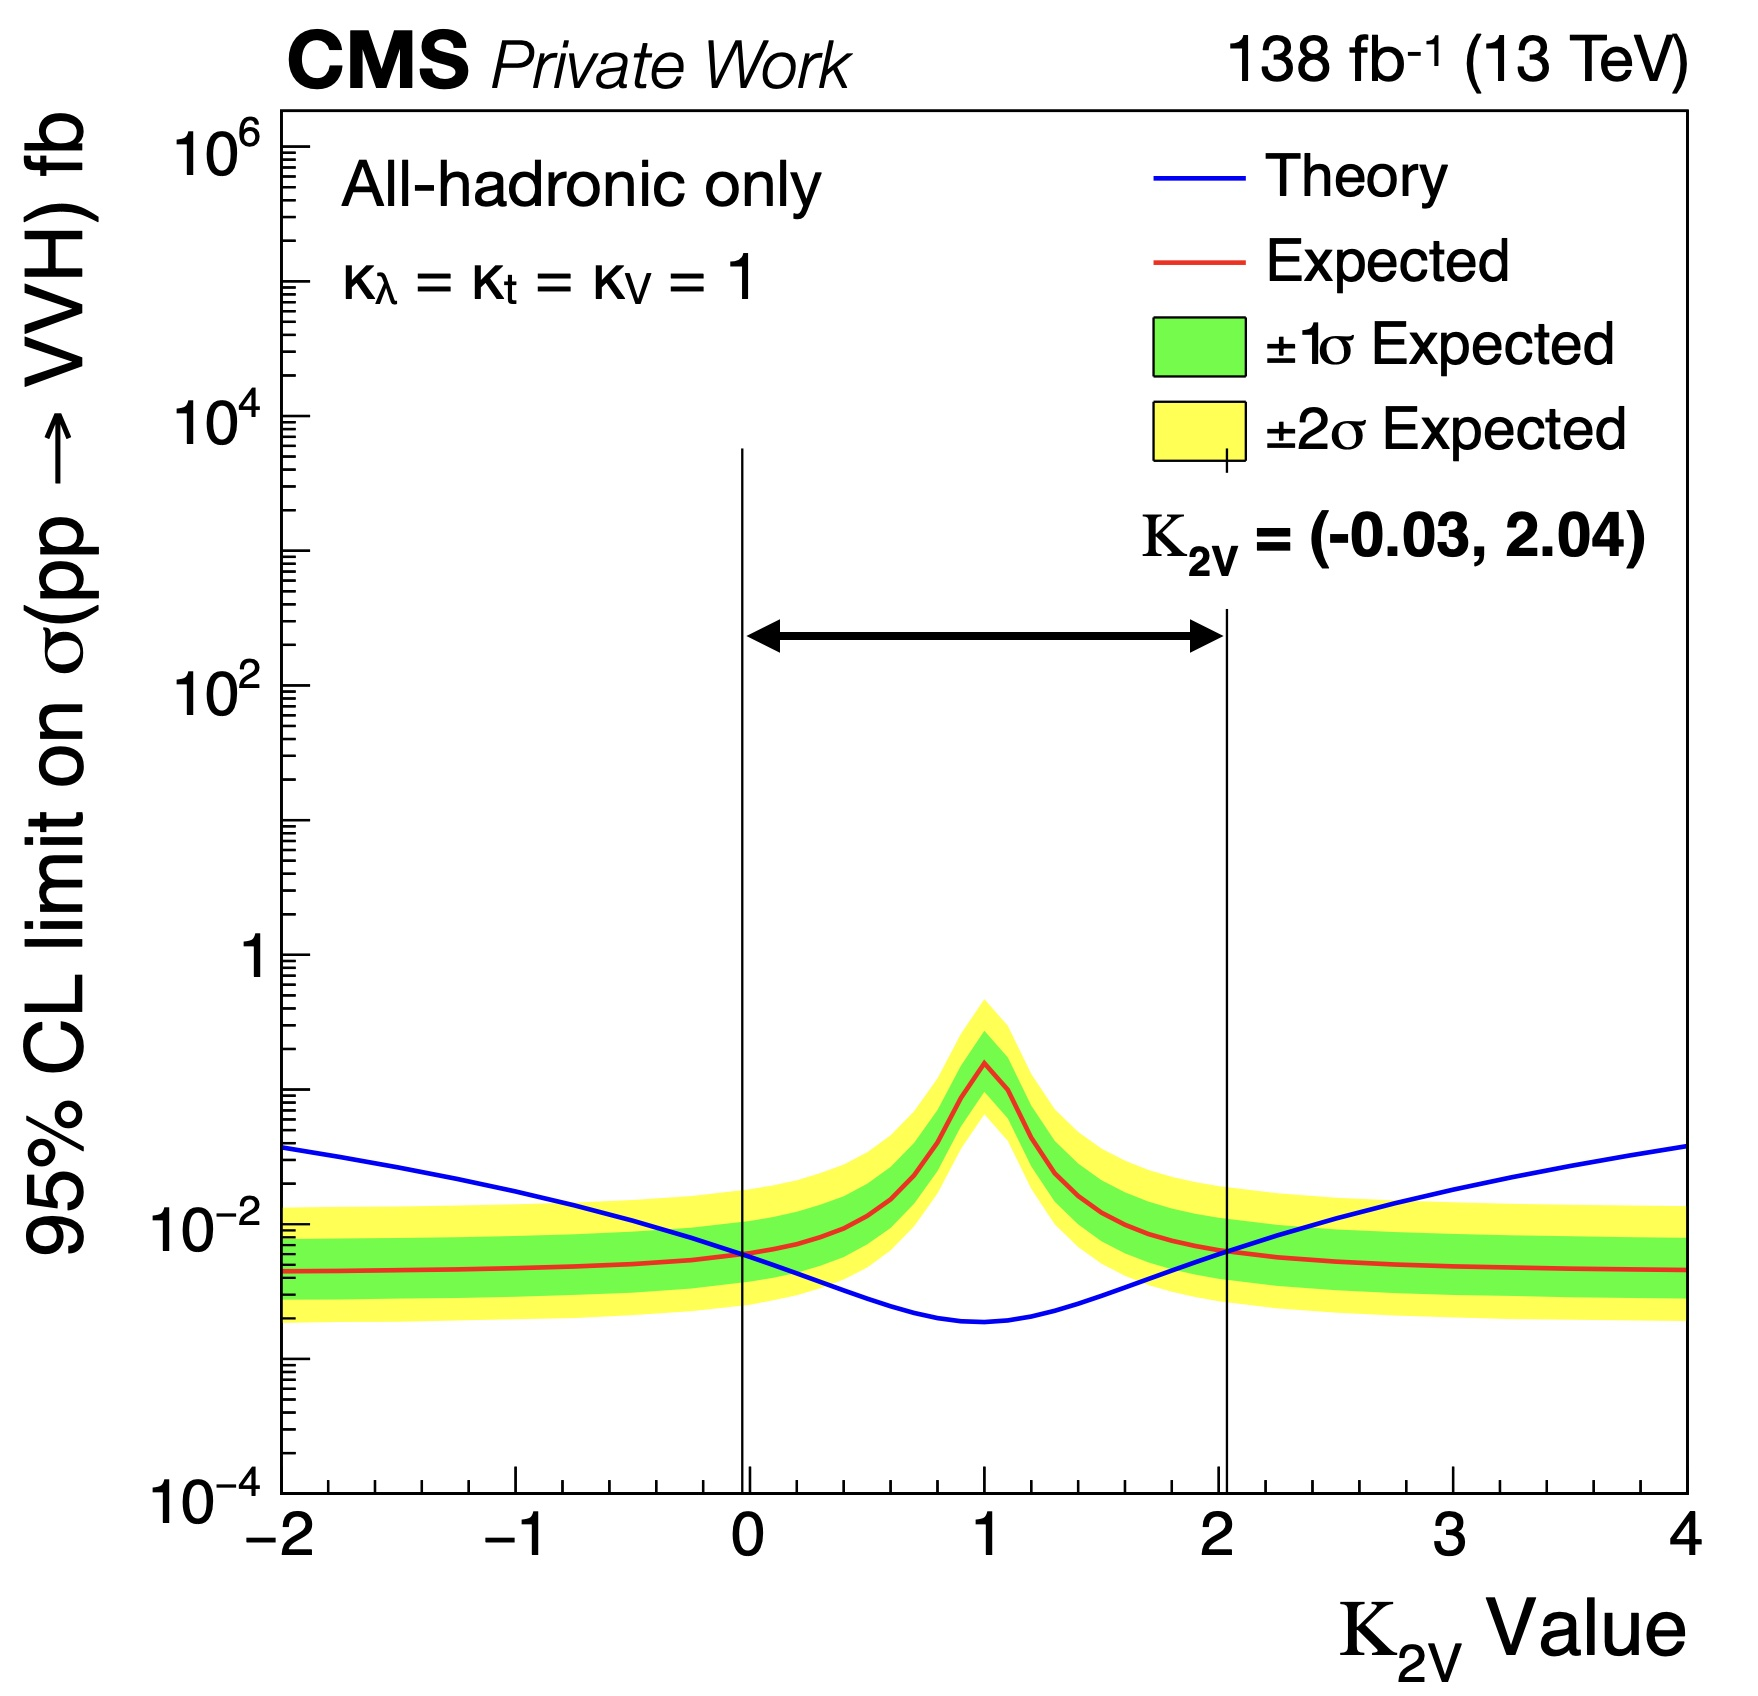
\includegraphics[width=0.45\textwidth]{fig/vbsvvh/k2v_limit_allhad.jpg}\label{fig:vbsvvh_limit_allhad}}\qquad
    \subfloat{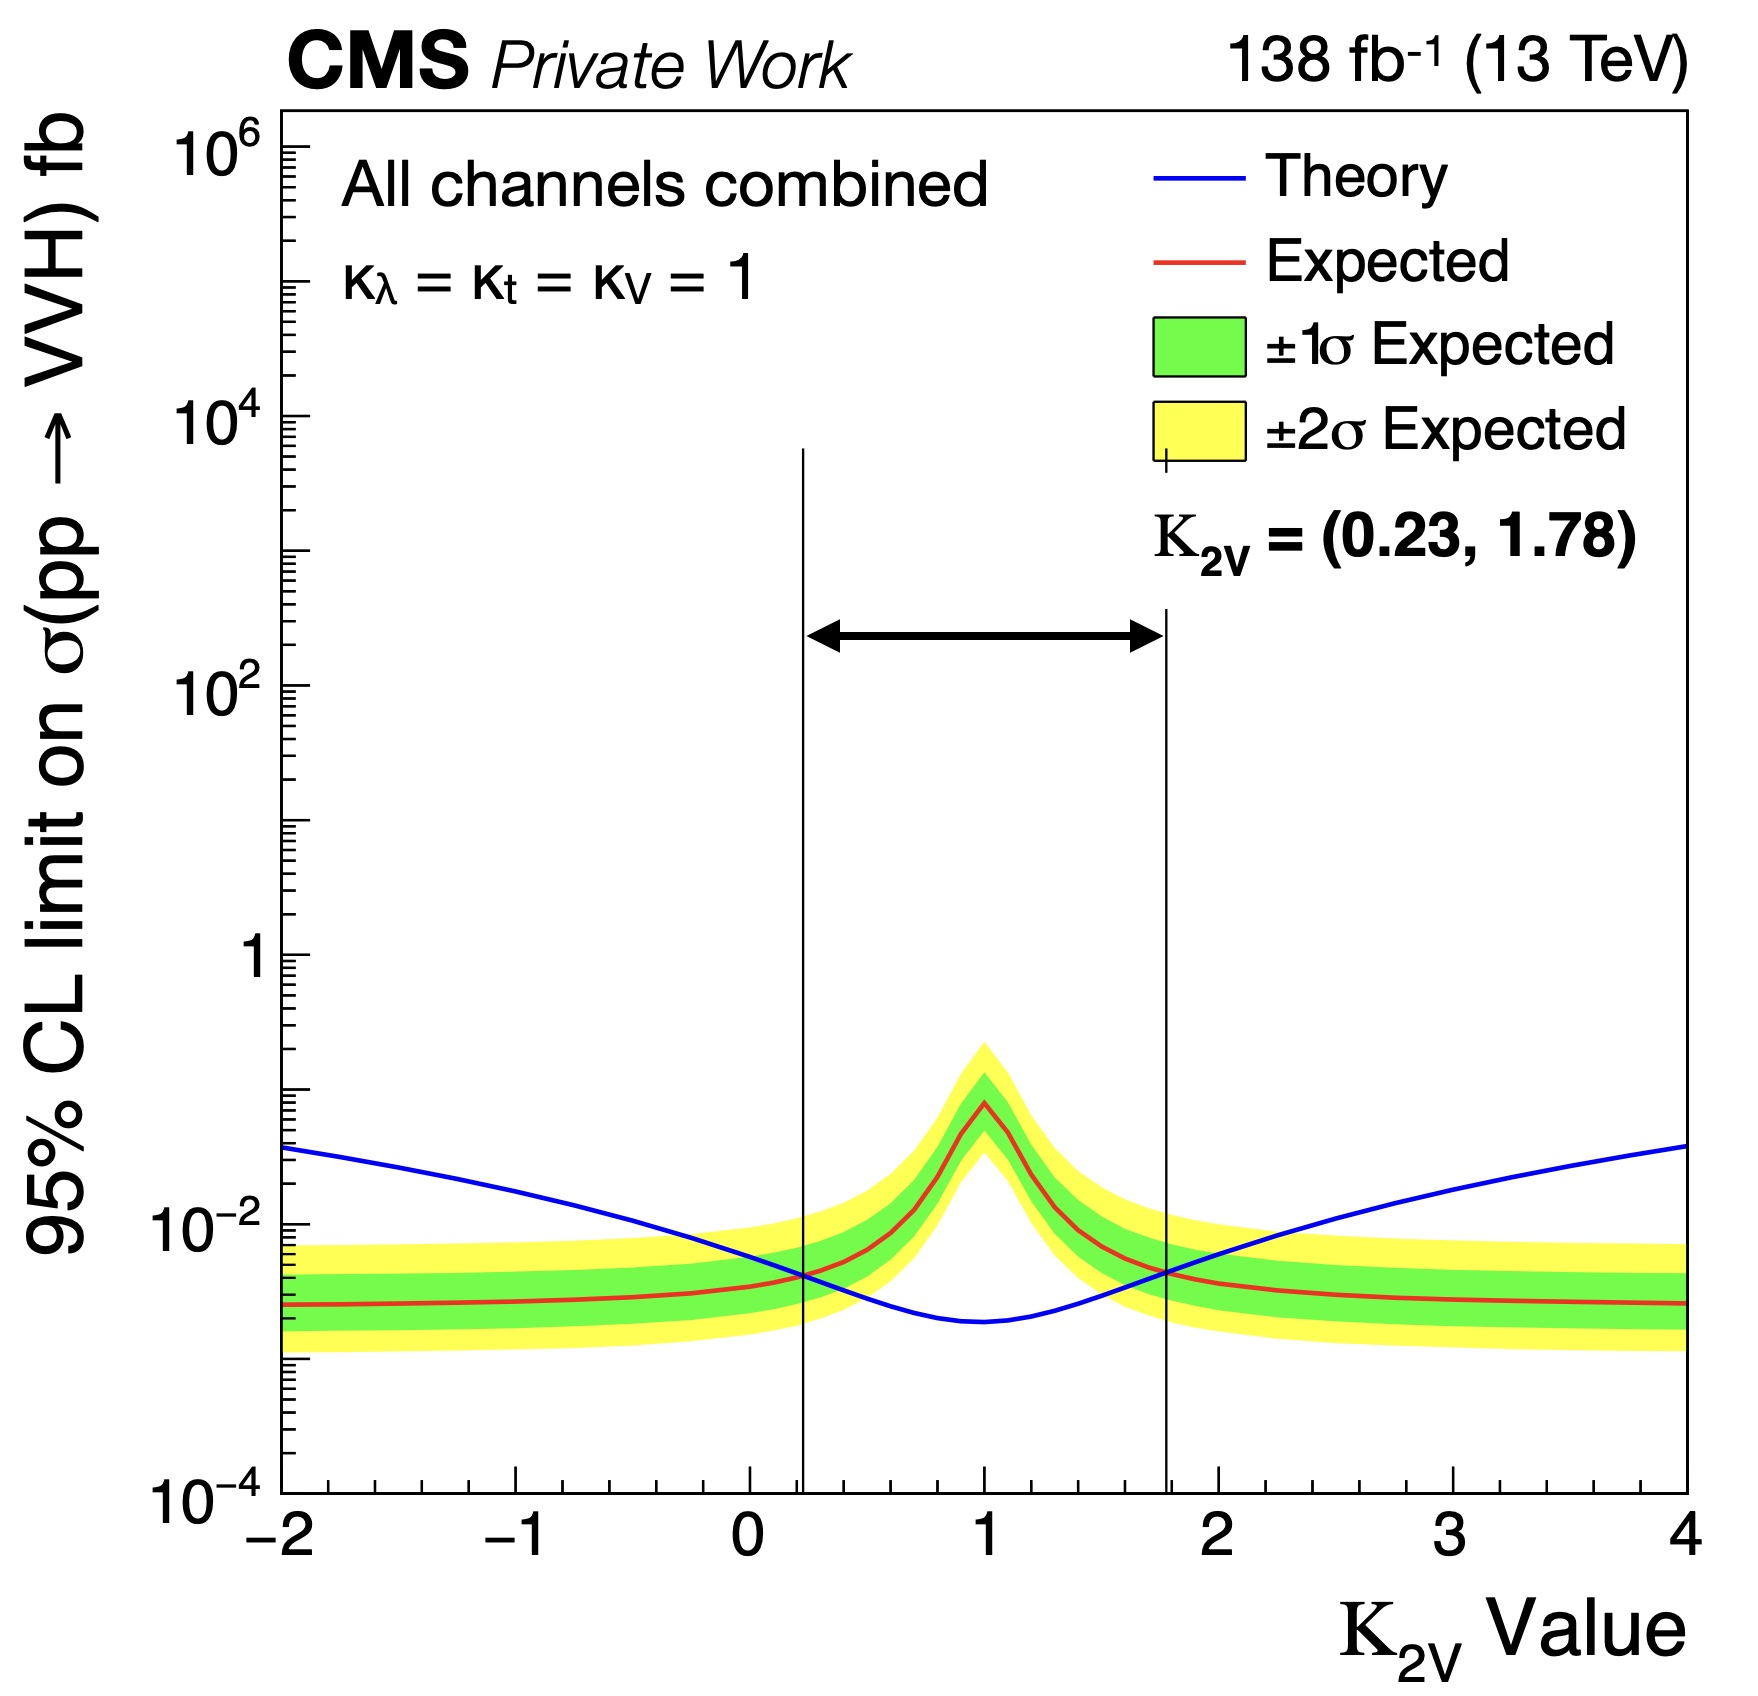
\includegraphics[width=0.45\textwidth]{fig/vbsvvh/k2v_limit_combined.jpg}\label{fig:vbsvvh_limit_combined}}
    \caption{The 95\% confidence level limit plotted as a function of \kVV for the all-hadronic channel (left) and all channels combined (right). 
    }
    \label{fig:vbsvvh_limit}
\end{figure}

\section{Acknowledgements}
This chapter is a partial reproduction of a paper being prepared for submission for publication. 
The work was made possible by the technical and administrative staff that operate and maintain the CERN accelerator complex, the LHC, CMS itself, and the worldwide LHC computing grid that provides data storage and processing capabilities for every LHC analysis. 
